\chapter{Searches for Supersymmetry at $\sqrt{s}=8\TeV$}
\label{ch:analysis8TeV}

\section{Event selection}
\label{sec:selection}
Events are selected at the L1 trigger level by requiring at least two
jets with $|\eta|<3$. At the HLT level, events are selected using
dedicated razor algorithms, consisting of a loose selection on \MR and
$\Rtwo$. Razor-specific triggers are used in the HLT in order to avoid
biases on the shapes of distributions from the SM background that are
introduced by requirements on more traditional selection variables
such as $\ETm$.  The razor triggers reject the majority of the SM
background, which mostly appears at low $\Rtwo$ and low $\MR$, while
retaining events in the signal-sensitive regions of the ($\MR$,
$\Rtwo$) plane. Two types of triggers are used: i) a hadronic razor
trigger, which selects events that contain at least two jets with
transverse momentum $\pt>64\GeV$ by applying threshold requirements on
$\Rtwo$, $\MR$, and their product; ii) a muon and electron razor
trigger, which selects events with at least one isolated electron or
muon with $\pt>12\GeV$ in combination with looser requirements on
$\Rtwo$, $\MR$, and their product. The trigger efficiency, evaluated
using a dedicated trigger, is measured to be $(95 \pm 5)\%$ and is
independent of $\Rtwo$ and $\MR$ for the events selected with the
baseline requirements described in Chapter~\ref{ch:kinematic}.

Following the trigger selection, events are required to contain at
least one reconstructed interaction vertex. If more than one vertex is
found, the one with the highest $\pt^2$ sum of associated tracks is
chosen as the interaction point for event reconstruction. Algorithms are
used to remove events with detector- and beam-related noise that can
mimic event topologies with high energy and large $\pt$
imbalance~\cite{Chatrchyan:2011tn,Chatrchyan:2012lia,Khachatryan:2014gga}.

The analysis uses a global event description based on the CMS particle
flow (PF) algorithm~\cite{PF1,PF2}. Individual particles (PF
candidates) are reconstructed by combining the information from the inner
tracker, the calorimeters, and the muon system. Five categories of PF
candidates are defined: muons, electrons, photons (including their
conversions to $\Pep\Pem$ pairs), charged hadrons, and neutral
hadrons. The contamination from other proton-proton collisions in the
same or in neighboring bunch crossings is reduced by discarding the
charged PF candidates not compatible with the interaction point. When
computing lepton isolation and jet energy, the corresponding
contamination from neutral particles is subtracted on average by
applying an event-by-event correction based on the jet-area
method~\cite{jetarea_fastjet,jetarea_fastjet_pu,JME-JINST}.

A ``tight'' lepton identification is used for muons and electrons,
consisting of requirements on isolation and track reconstruction
quality. For electrons, the shape and position of the energy deposit
in the electromagnetic calorimeter is used to further reduce the contamination from
hadrons~\cite{Chatrchyan:2013iaa}. For events with one identified
tight lepton, additional muons or electrons are identified through a
``loose'' lepton selection, characterized by a relaxed isolation
requirement~\cite{Chatrchyan:2013mxa}. Tight leptons are
required to have $\pt>15$\GeV and loose leptons $\pt>10$\GeV.

Jets are reconstructed by clustering the PF candidates with the
\textsc{FastJet}~\cite{fastjet} implementation of the anti-\kt~\cite{antikt} algorithm with the distance parameter $R=0.5$. We
select events containing at least two jets with $\pt>80$\GeV and
$\abs{\eta}<2.4$, representing a tighter version of the L1 jet selection criterion. The $\pt$
imbalance in the event, $\ptvecmiss$, is the
negative of the sum of the $\ptvec$ of the PF candidates in the
event. Its magnitude is referred to as $\ETm$. For each event, the $\ptvecmiss$ and the
four-momenta of all the jets with $\pt>40$\GeV and $\abs{\eta}<2.4$ are
used to compute the razor variables, as described in
Section~\ref{sec:razVar}.

The medium working point of the combined secondary vertex
algorithm~\cite{btag8TeV} is used for b-jet tagging. The \PQb-tagging
efficiency and mistag probability are measured from data control
samples as a function of the jet $\pt$ and $\eta$. Correction factors
are derived for Monte Carlo (MC) simulations through comparison of the
measured and simulated \PQb-tagging efficiencies and mistag rates found
in these control samples~\cite{btag8TeV}.

Events with no \PQb-tagged jet are discarded, a criterion motivated by
the natural SUSY signatures described in Section~\ref{sec:sms}. A tighter
requirement ($\geq$2 \PQb-tagged jets) is imposed on events without an
identified tight lepton and fewer than four jets. This requirement reduces the
expected background from SM production of $\cPZ(\to\nu\bar\nu)$+jets
events to a negligible level.


\section{Box definitions}
\label{sec:razVar}

The selected events are categorized into the different razor boxes according to
their event content as shown in Table~\ref{tab:boxDef}. In the table,
the boxes are listed according to the filling order, from the first
(at the top of the table) to the last (at the bottom). If an event
satisfies the requirements of two or more boxes, the event is assigned
to the first listed box to ensure the boxes correspond to disjoint samples.

The events in the single-lepton and two-lepton boxes are recorded
using the electron and muon razor trigger. The remaining two boxes, generically
referred to as ``hadronic'' boxes, contain events recorded using the
hadronic razor trigger.

In the two-lepton boxes, the ($\MR$, $\Rtwo$)
distribution of events with at least one \PQb-tagged jet is studied. For
the other boxes, the data are binned according to the \PQb-tagged jet
multiplicity: 1 \PQb-tag, 2 \PQb-tags, and $\geq$3 \PQb-tags.

\begin{table*}[ht!]
\centering
 \caption{Kinematic and multiplicity requirements defining the nine
 razor boxes. Boxes are listed in order of event filling priority.
 \label{tab:boxDef}}
\resizebox{\textwidth}{!}{
\begin{tabular}{ccccc}
Box & Lepton & \PQb-tag & Kinematic & Jet \\
\hline
 \multicolumn{5}{c}{Two-lepton boxes}\\
\hline
\multirow{2}{*}{MuEle} & $\geq$1 tight electron and & \multirow{6}{*}{$\geq$1 \PQb-tag} & \multirow{2}{*}{} & \multirow{6}{*}{$\geq$2 jets}\\
& $\geq$1 loose muon & & & \\
\cline{1-2}
\multirow{2}{*}{MuMu} & $\geq$1 tight muon and & & ($\MR >300$\GeV and $\Rtwo > 0.15$) and & \\
& $\geq$1 loose muon & & ($\MR > 350$\GeV  or $\Rtwo > 0.2$) & \\
\cline{1-2}
\multirow{2}{*}{EleEle} & $\geq$1 tight electron and & & & \\
& $\geq$1 loose electron& & & \\
\hline
\multicolumn{5}{c}{Single-lepton boxes}\\
\hline
MuMultiJet & 1 tight muon & \multirow{4}{*}{$\geq$1 \PQb-tag} & & \multirow{2}{*}{$\geq$4 jets} \\
%\cline{1-2}
EleMultiJet &1 tight electron & & ($\MR > 300$\GeV and $\Rtwo > 0.15$) and & \\
%\cline{1-2}
\cline{5-5}
MuJet & 1 tight muon & & ($\MR > 350$\GeV or $\Rtwo > 0.2$) & \multirow{2}{*}{2 or 3 jets}\\
%\cline{1-2}
EleJet & 1 tight electron & & &  \\
\hline
\multicolumn{5}{c}{Hadronic boxes}\\
\hline
MultiJet & none & $\geq$1 \PQb-tag & ($\MR > 400$\GeV and $\Rtwo > 0.25$) and &$\geq$4 jets\\
%\cline{1-3}
%\cline{5-5}
$\geq$2 \PQb-tagged jet & none & $\geq$2 \PQb-tag &  ($\MR > 450$\GeV or $\Rtwo > 0.3$) & 2 or 3 jets\\
\end{tabular}}
\end{table*}

A baseline kinematic requirement is applied to define the region in
which we search for a signal:
\begin{itemize}
\item $\MR>400$\GeV and $\Rtwo>0.25$ for the hadronic boxes;
\item $\MR>300$\GeV and $\Rtwo>0.15$ for the other boxes.
\end{itemize}
The tighter baseline selection for the hadronic boxes is a consequence
of the tighter threshold used for the hadronic razor trigger. The
kinematic plane defined by the baseline selection is divided into three
regions (see Fig.~\ref{fig:regions}):
\begin{itemize}
\item Low \MR sideband: $400<\MR<550$\GeV
 and $\Rtwo>0.30$ for the hadronic boxes;
 $300<\MR<450$\GeV and $\Rtwo>0.20$ for the other
 boxes.
\item Low  \Rtwo sideband: $\MR>450$\GeV and
  $0.25<\Rtwo<0.30$ for the hadronic boxes;
  $\MR>350$\GeV and $0.15<\Rtwo<0.20$ for the other
  boxes.
\item Signal-sensitive region: $\MR>550$\GeV and
 $\Rtwo>0.30$ for the hadronic boxes; $\MR>450$\GeV
 and $\Rtwo>0.20$ for the other boxes.
\end{itemize}
The bottom left corner of the razor plane, not included in any of the
three regions, is excluded from the analysis. Given this selection,
the multijet background from quantum chromodynamics processes is
reduced to a negligible level due to the fact that these processes
typically peak at $\Rtwo\approx0$ and fall exponentially for
larger values of $\Rtwo$~\cite{razorPRL,razorPRD}.

\begin{figure}[ht!]
\centering
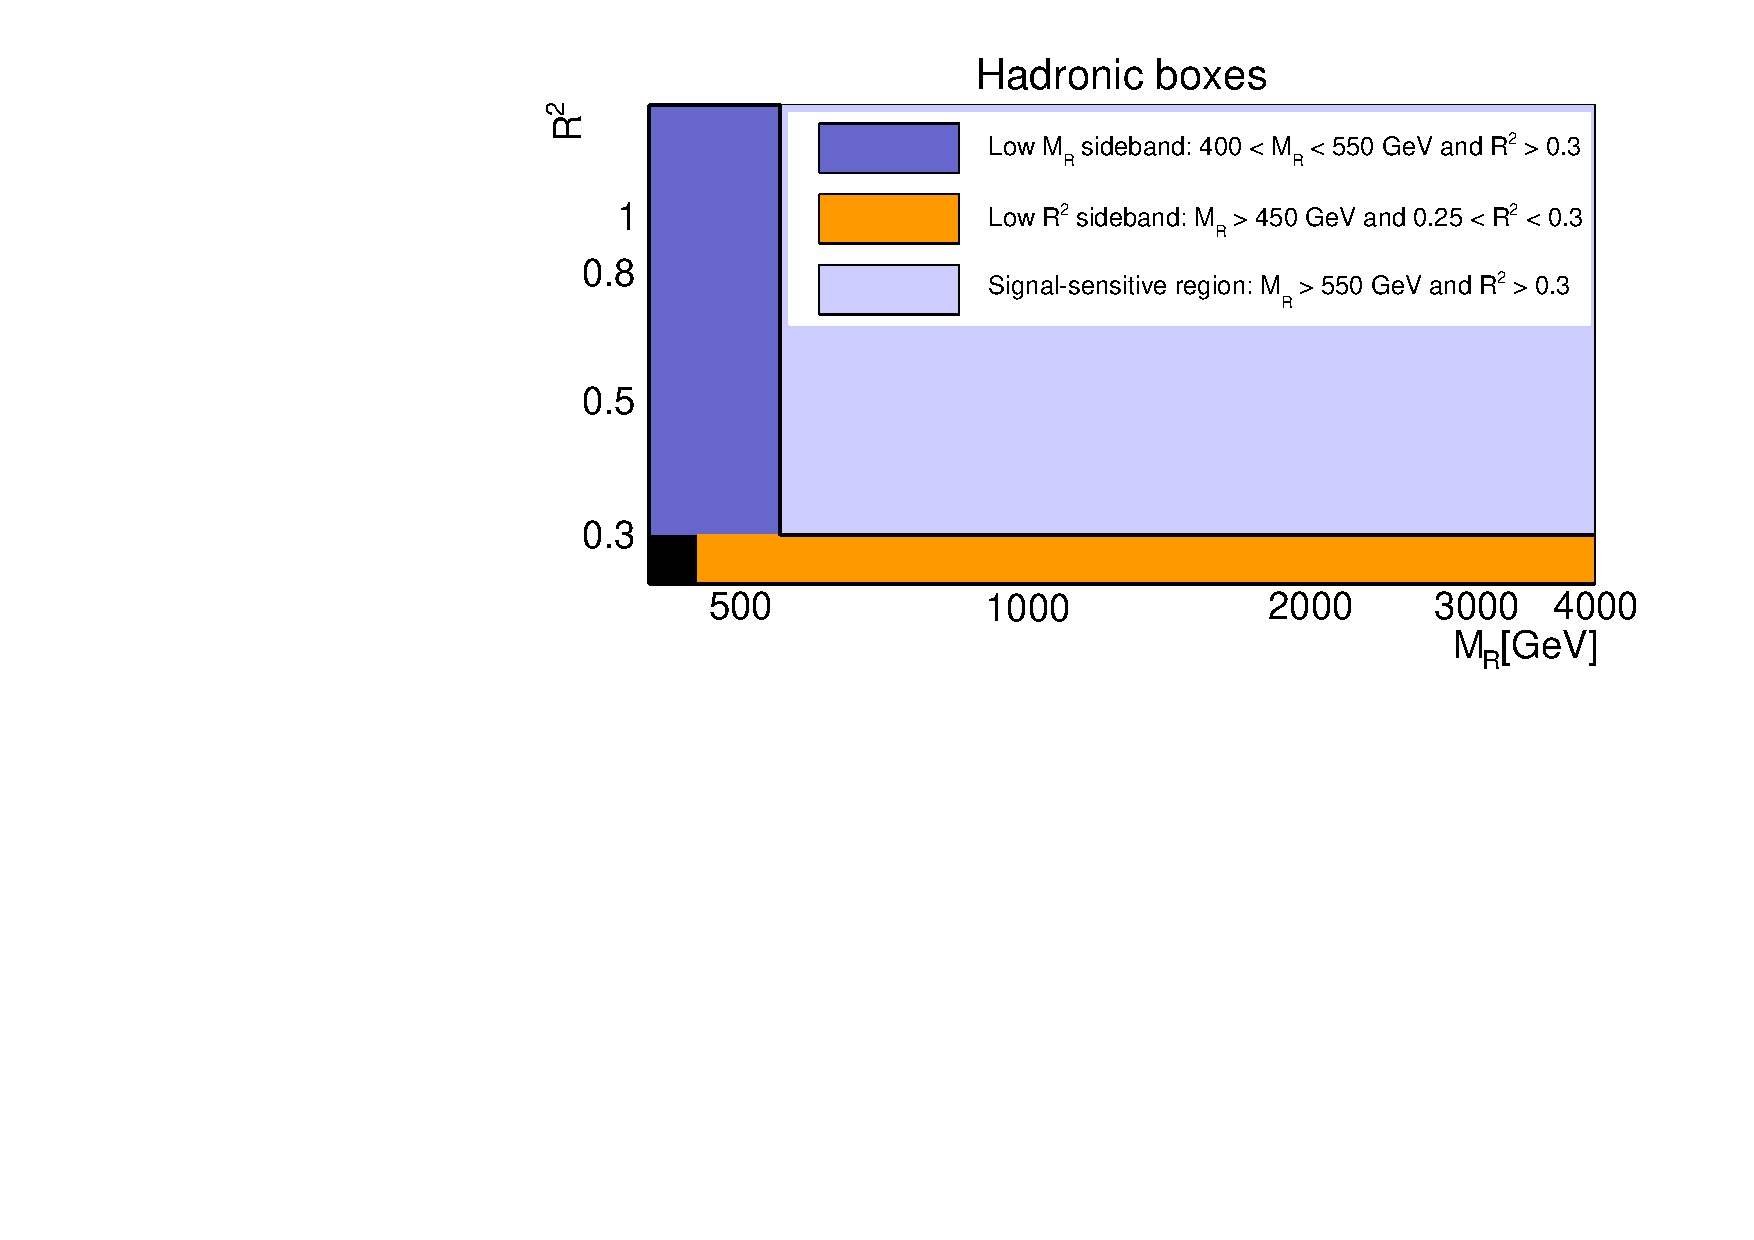
\includegraphics[width=0.49\textwidth]{figs/analysis8TeV/SidebandL_MultiJet.pdf}
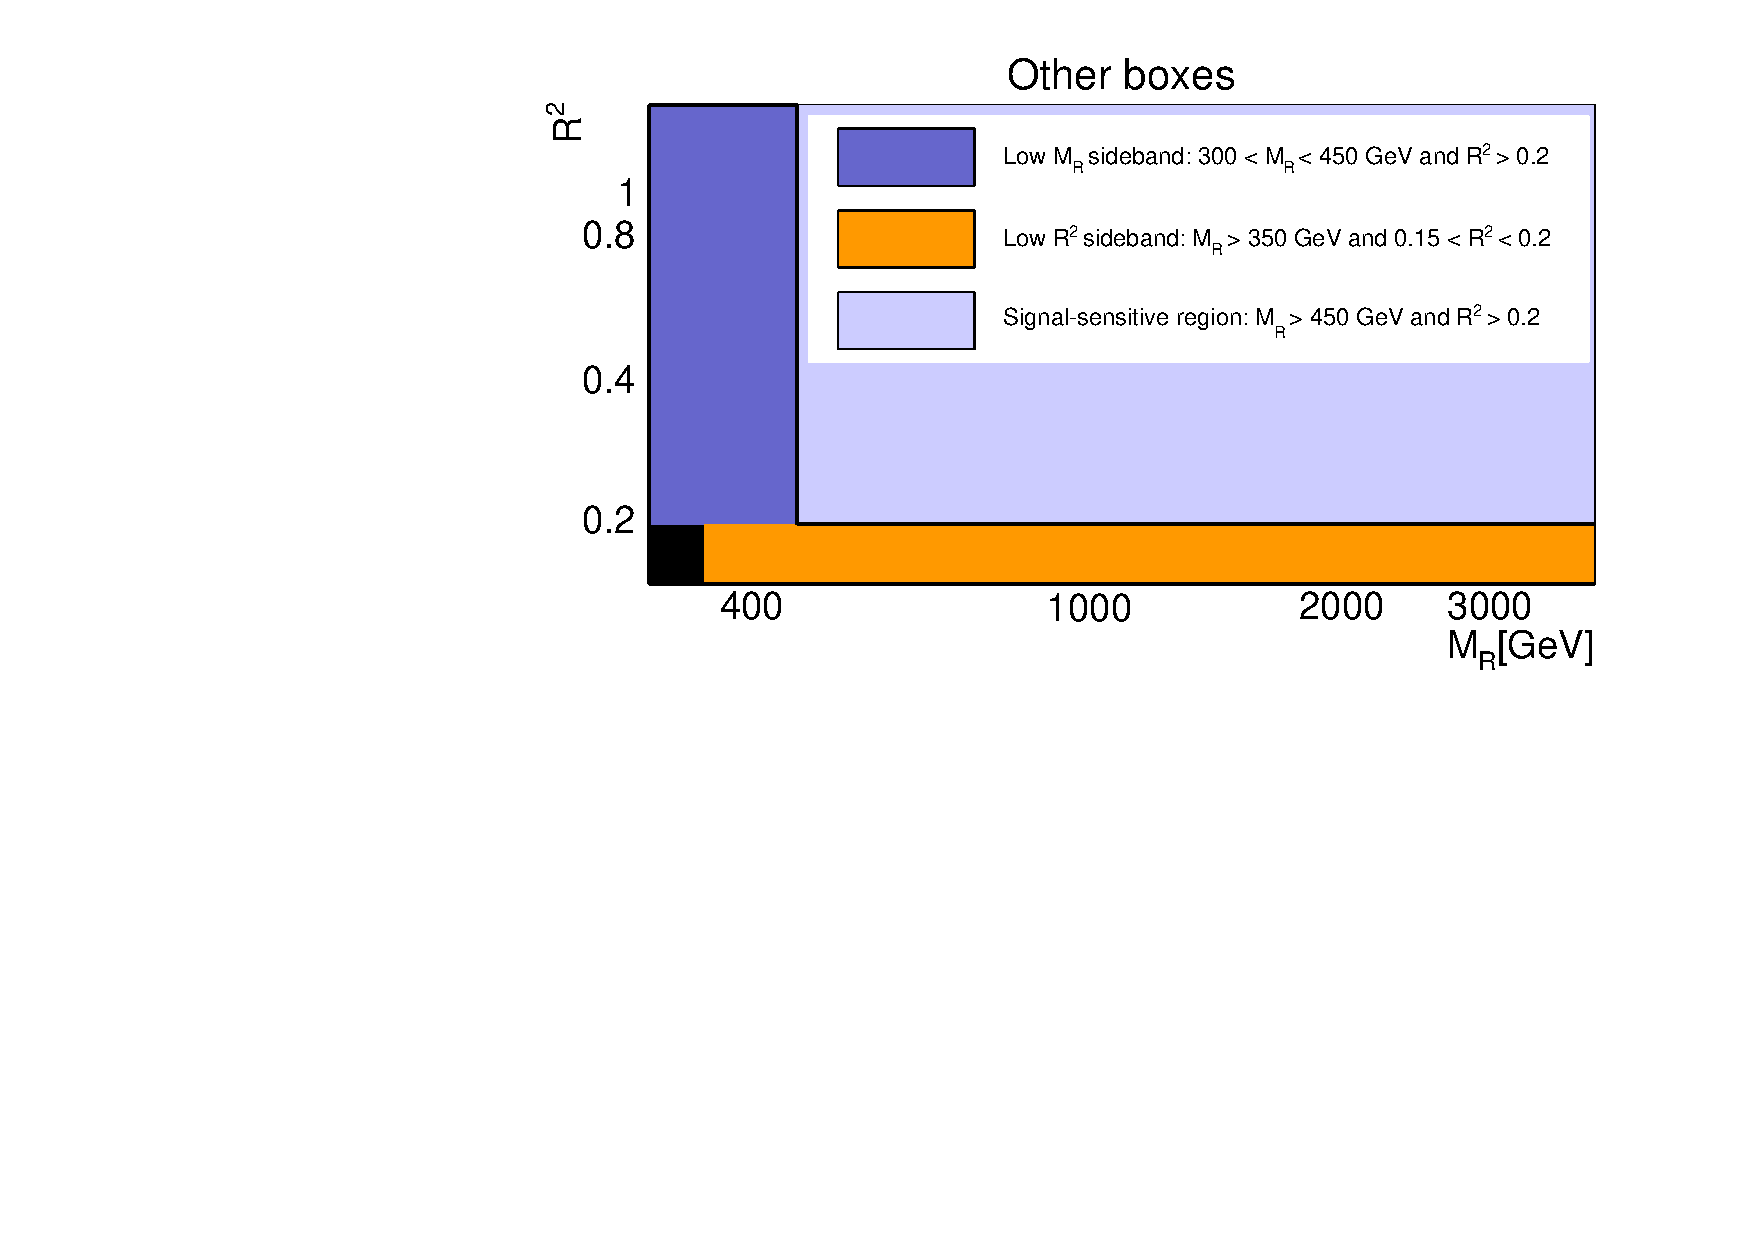
\includegraphics[width=0.49\textwidth]{figs/analysis8TeV/SidebandL_Mu.pdf}
\caption{\label{fig:regions} Definition of the sideband and the
 signal-sensitive regions used in the analysis, for (left) the hadronic
 boxes and (right) the other boxes.}
\end{figure}

\section{Modeling of the standard model backgrounds}
\label{sec:bmodel}
Under the hypothesis of no contribution from new-physics processes,
the event distribution in the considered portion of the
($\MR$, $\Rtwo$) plane can be described by the sum of
the contributions from SM $\cPV$+jets events (where
$\cPV$ indicates a $\PW$ or $\cPZ$ boson) and SM top quark-antiquark and
single-top events, where the events with a top quark are generically
referred to as the $\ttbar$ contribution. Based on MC studies, the
contributions from other processes are determined to be
negligible.

We study each of these processes using MC samples, generated with the
\MADGRAPH v5
simulation~\cite{Alwall:2011uj,Alwall:2014hca}. Parton shower and
hadronization effects are included by matching events to the \PYTHIA v6.4.26 simulation~\cite{Sjostrand:2006za} using the MLM
algorithm~\cite{Hoche:2006ph}. The events are processed by a
\GEANT-based~\cite{G4} description of the CMS apparatus in order to
account for the response of the detector.

Once normalized to the NLO inclusive cross
section and the integrated luminosity, the absolute yield of the
$\cPV$+jets events contribution satisfying the event selection is found
to be negligible in all of the two-lepton boxes. In the remaining boxes,
its contribution to the total SM background is found to be
approximately 25\%. The contribution of $\cPV$+jets events in
the $\geq$2 \PQb-tag and the $\geq$4 jet sample is found to be
negligible. The remainder of the background in each box originates
from $\ttbar$ events.

\subsection{Empirical Razor Function}
Based on the study of the data collected at $\sqrt{s}=7\TeV$ and the
corresponding MC samples~\cite{razorPRL,razorPRD}, the two-dimensional
probability density function
$P_\mathrm{SM}(\MR,\Rtwo)$ for each SM process is
found to be well described by the empirical function
\begin{equation}
 f(\MR,\Rtwo) =  \bigl[b(\MR-{\MRz})^{1/n}(\Rtwo-{\Rtwoz})
  ^{1/n}-1\bigr]\re^{-bn(\MR-{\MRz})^{1/n}(\Rtwo-{\Rtwoz})
    ^{1/n}} ,
\label{eq:razFun}
\end{equation}
where $b$, $n$, $\MRz$, and $\Rtwoz$ are free
parameters of the background model. 

For $n=1$, this function recovers the two-dimensional exponential function used for previous
studies~\cite{razorPRL,razorPRD}. The original motivation is detailed
in the cited papers, but a quick summary follows. There is an observed
correlation between the two razor variables such that after a baseline
selection $\MR>\MR^{\mathrm{min}}$ and $\Rtwo>\Rtwo_{\mathrm{min}}$, the distributions of the SM backgrounds
exhibit an exponential behavior in $\Rtwo$ ($\MR$) when integrated over
$(\MR)$, ($\Rtwo$):
\begin{align}
 \int^{\infty}_{\Rtwo_{\mathrm{min}}} P_\mathrm{SM}(\MR,\Rtwo)
  \mathrm{d}\Rtwo &\propto e^{-(r_0 + r_1\Rtwo_{\mathrm{min}})M_R}~,\\
 \int^{\infty}_{\MR^{\mathrm{min}}} P_\mathrm{SM}(\MR,\Rtwo)
  \mathrm{d}\MR &\propto  e^{-(m_0+ m_1\MR^{\mathrm{min}})\Rtwo}~,
\label{eq:2dcorrelation}
\end{align}
where $r_0$, $r_1$, $m_0$, and $m_1$ are interrelated exponential parameters.
This behavior for QCD multijets background is illustrated in
Fig.~\ref{fig:qcdfit}. The empricial function in Eqn.~\ref{eq:razFun} with
$n=1$ perfectly replicates this behavior and the exponential parameters can be identified with
the empirical function's parameters, namely $r_0 = - b\Rtwoz$, $m_0 = - b\MRz$, and $r_1=m_1=b$.

\begin{figure}[tb!]
\centering
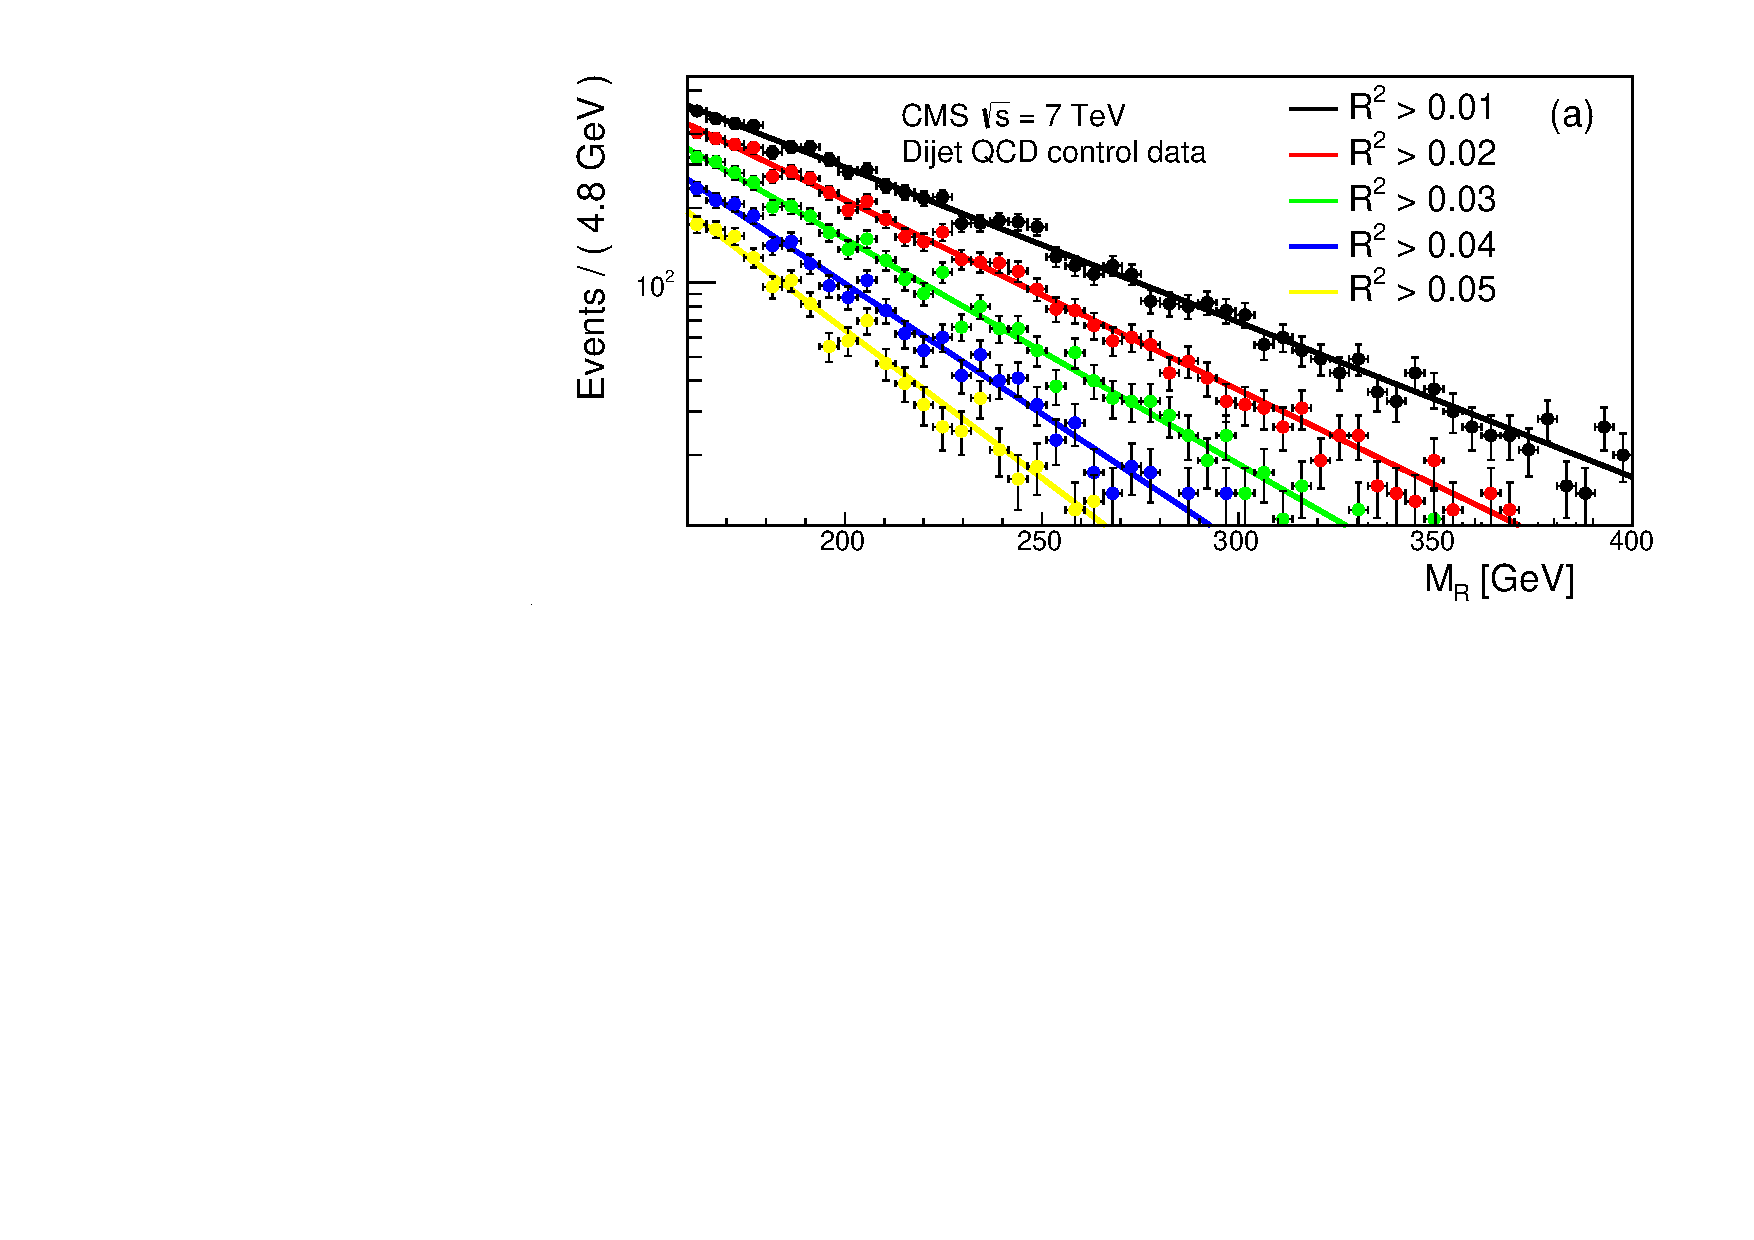
\includegraphics[width=0.49\textwidth]{figs/analysis8TeV/qcd-mr-prd.pdf}
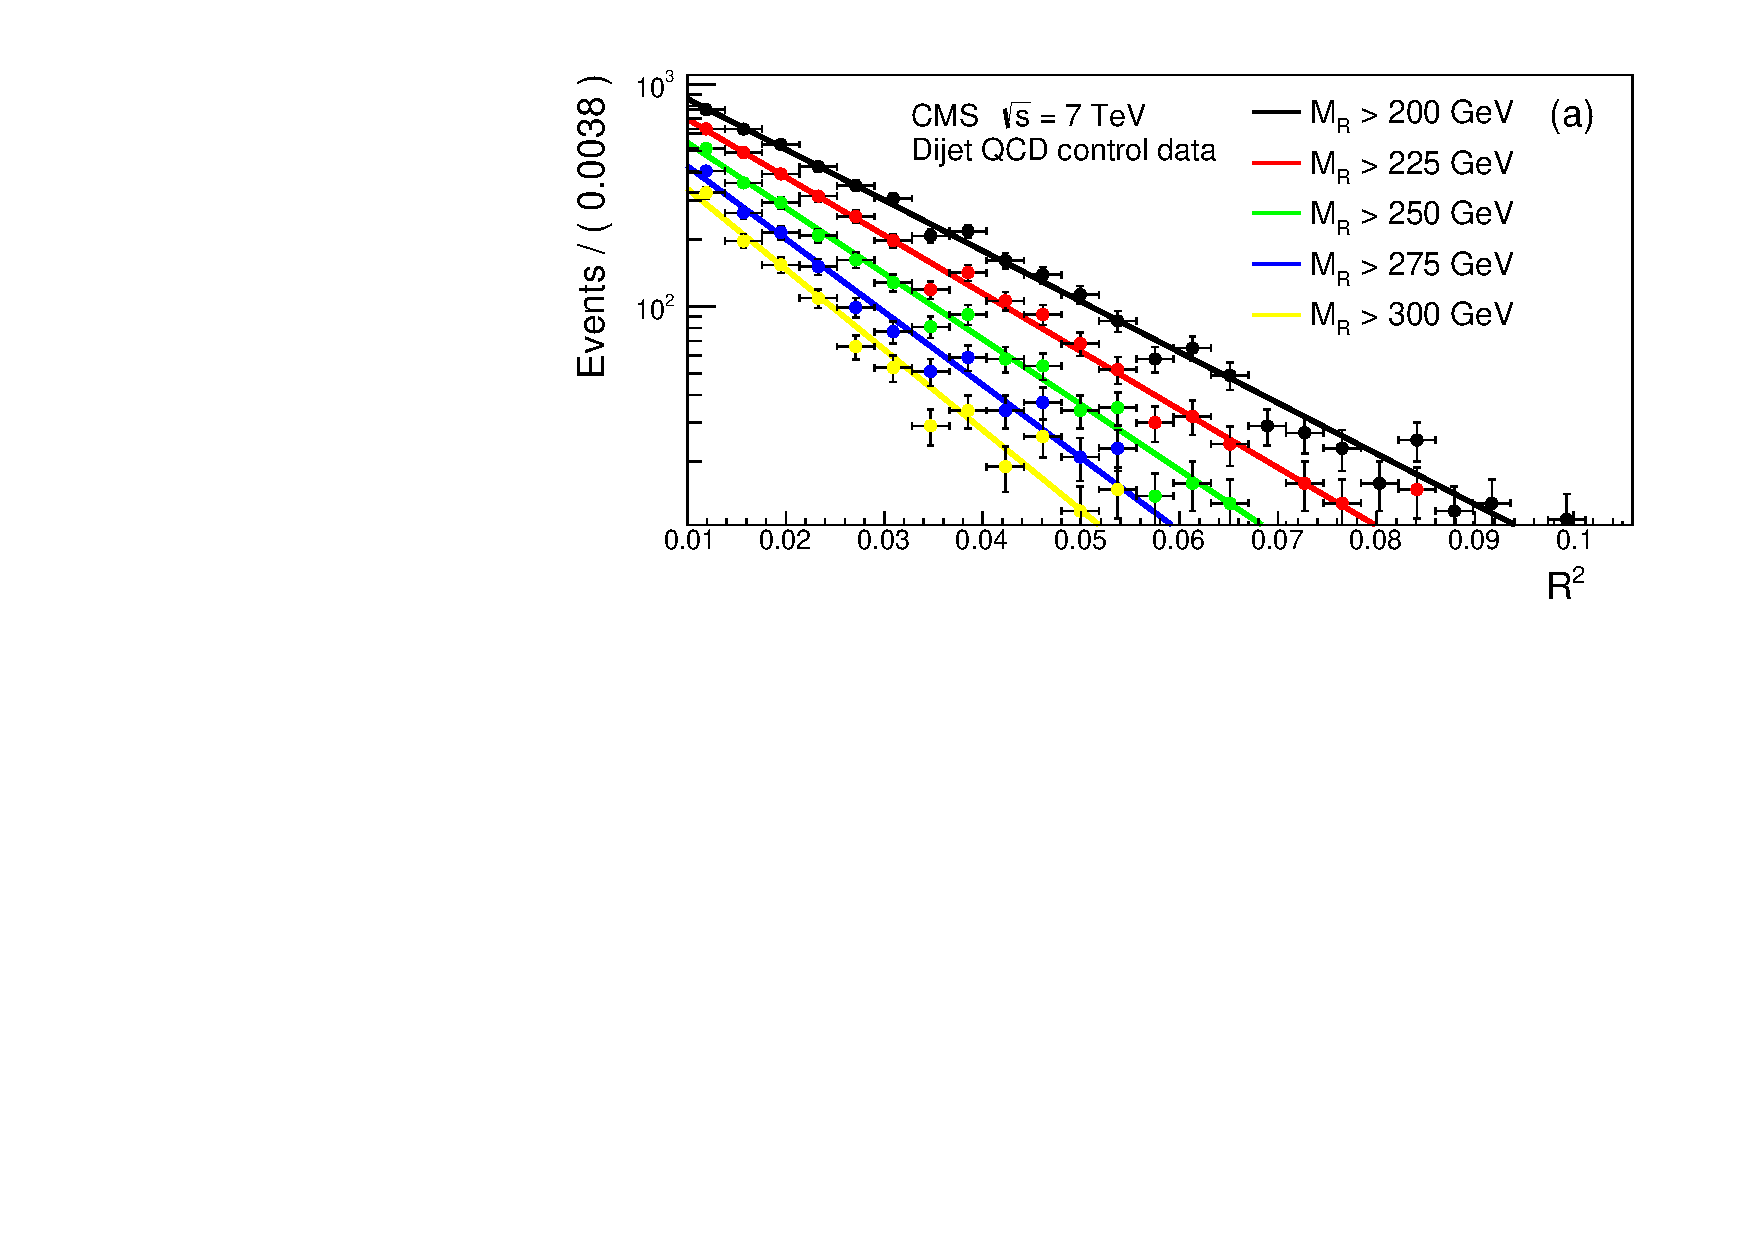
\includegraphics[width=0.49\textwidth]{figs/analysis8TeV/qcd-rsq-prd.pdf}\\
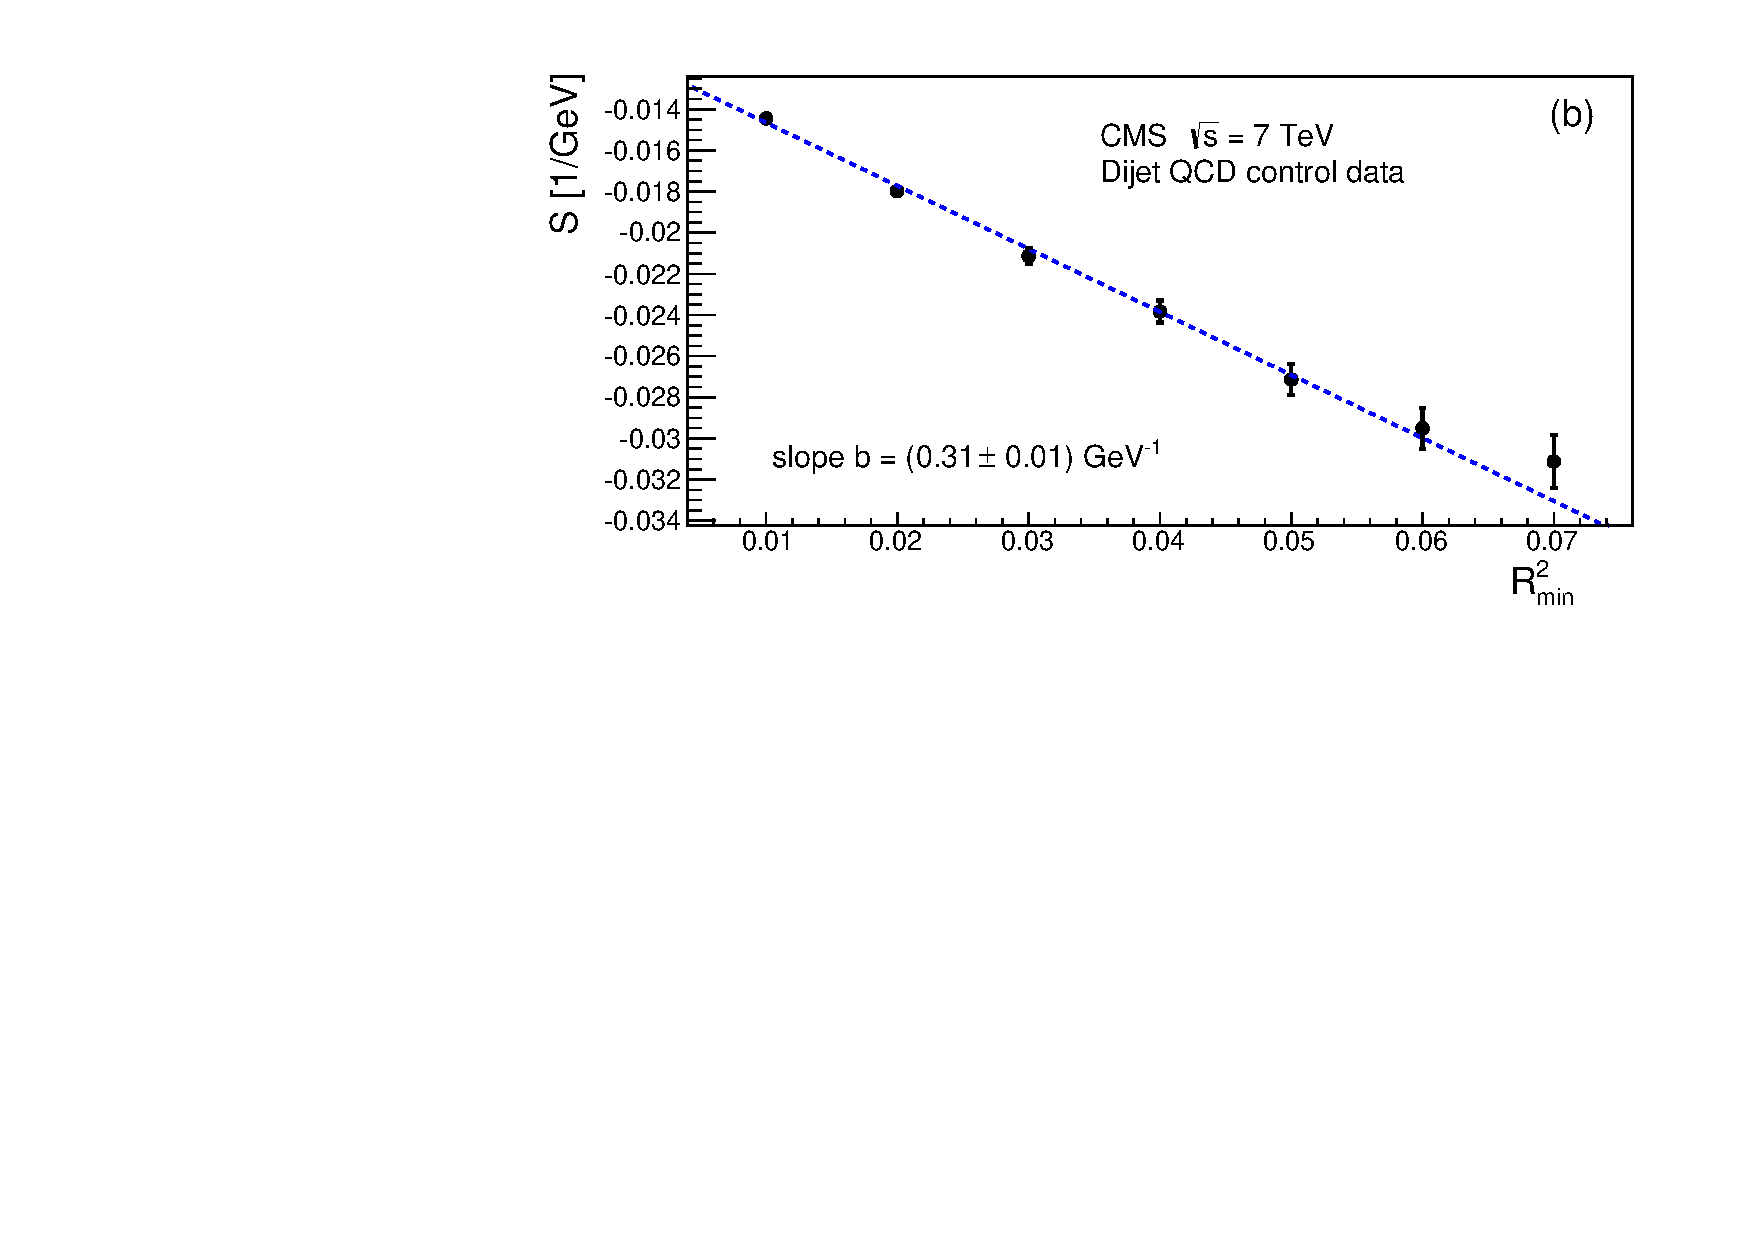
\includegraphics[width=0.49\textwidth]{figs/analysis8TeV/qcd-slopeMR-prd.pdf}
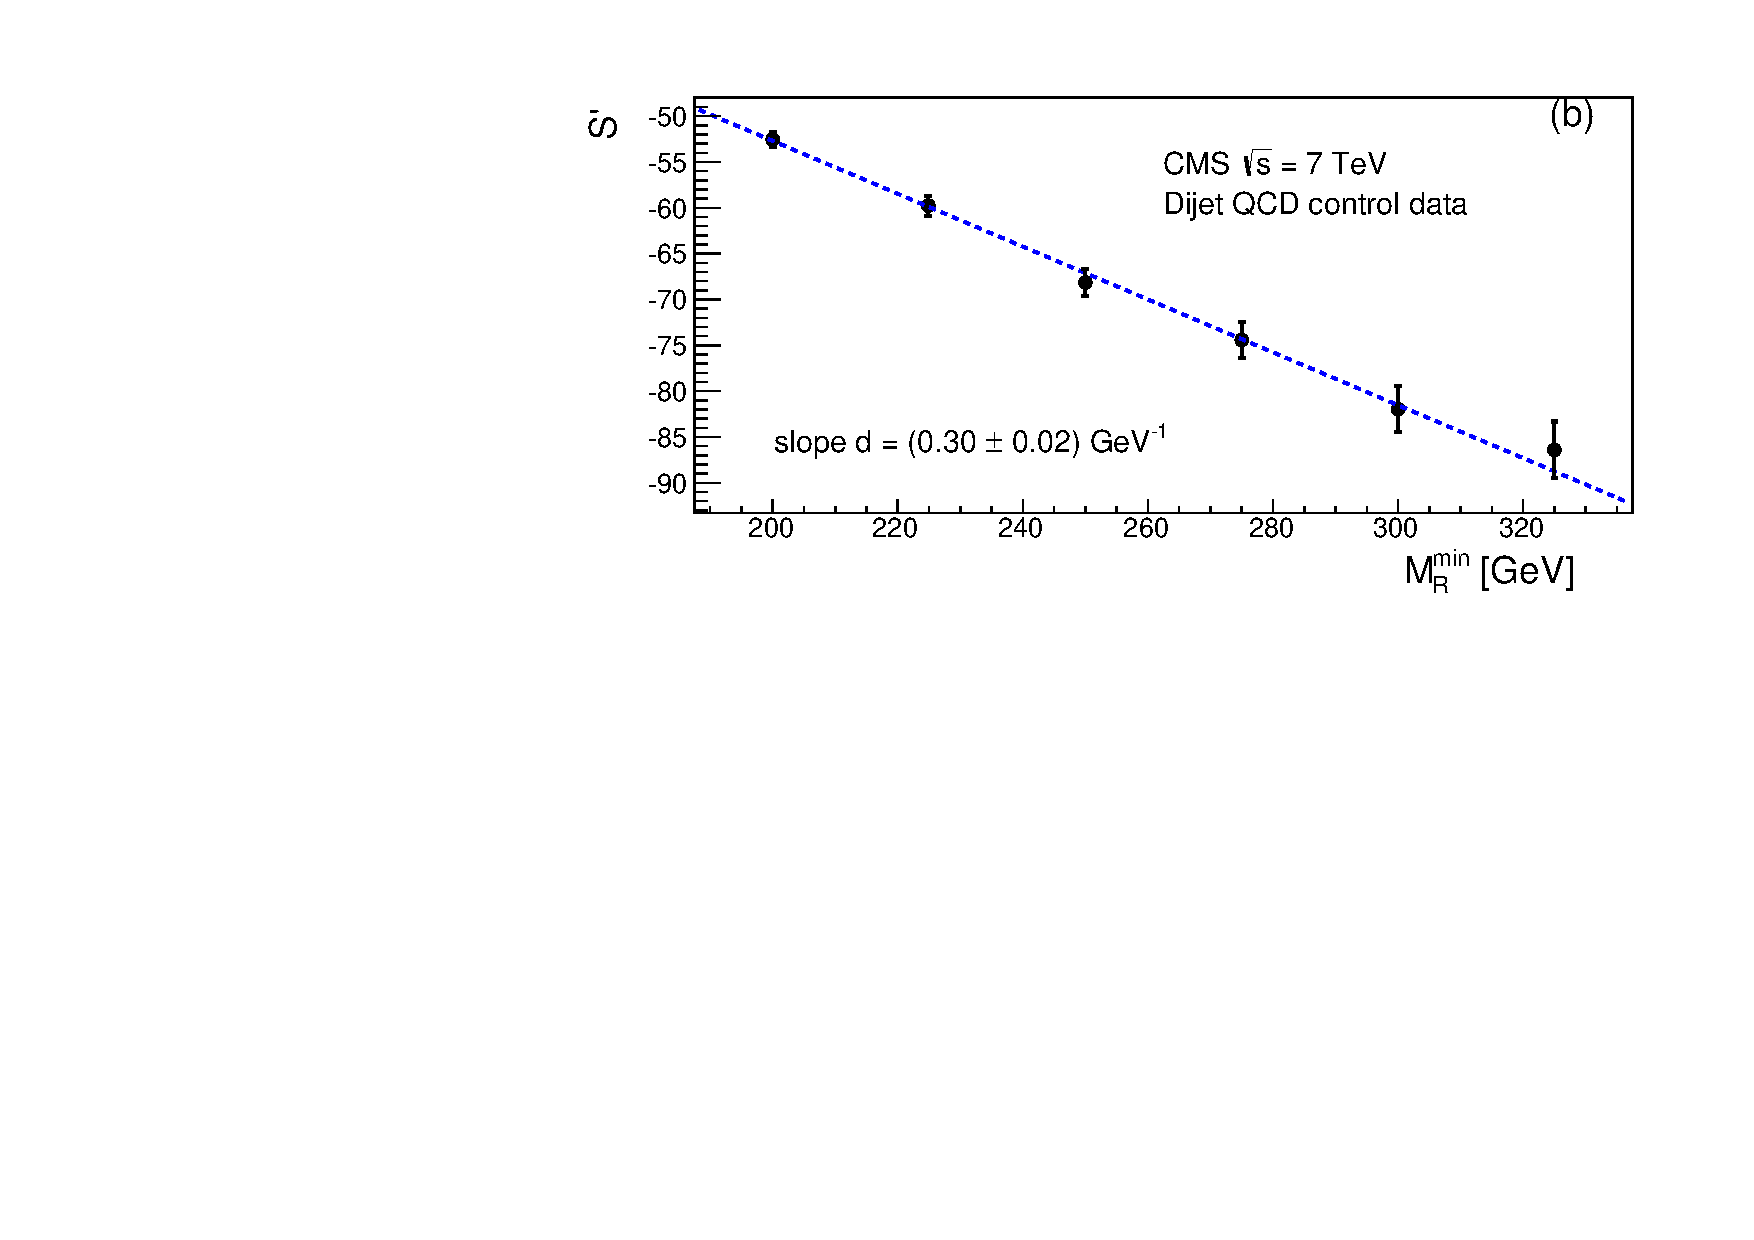
\includegraphics[width=0.49\textwidth]{figs/analysis8TeV/qcd-slopeR-prd.pdf}
\caption{QCD multijet events collected by CMS at $\sqrt{s}=7\TeV$
  demonstrate the two-dimensional correlation between $\MR$ and
  $\Rtwo$ that motivates the original functional form.\label{fig:qcdfit}}
\end{figure}

To account for the possibility of non-exponential tails of the SM
backgrounds, the $\sqrt{s}=7\TeV$ search invoked two copies of the
empirical function with $n=1$ to model each SM background. 
For the $\sqrt{s}=8\TeV$ search, we take a different approach by using
only one instance of the function, but allowing the $n$ parameter to deviate
from $1$. Fig.~\ref{fig:twoexp} illustrates the similarity between using two exponential components and using one
instance of the generalized function.

\begin{figure}[tb!]
\centering
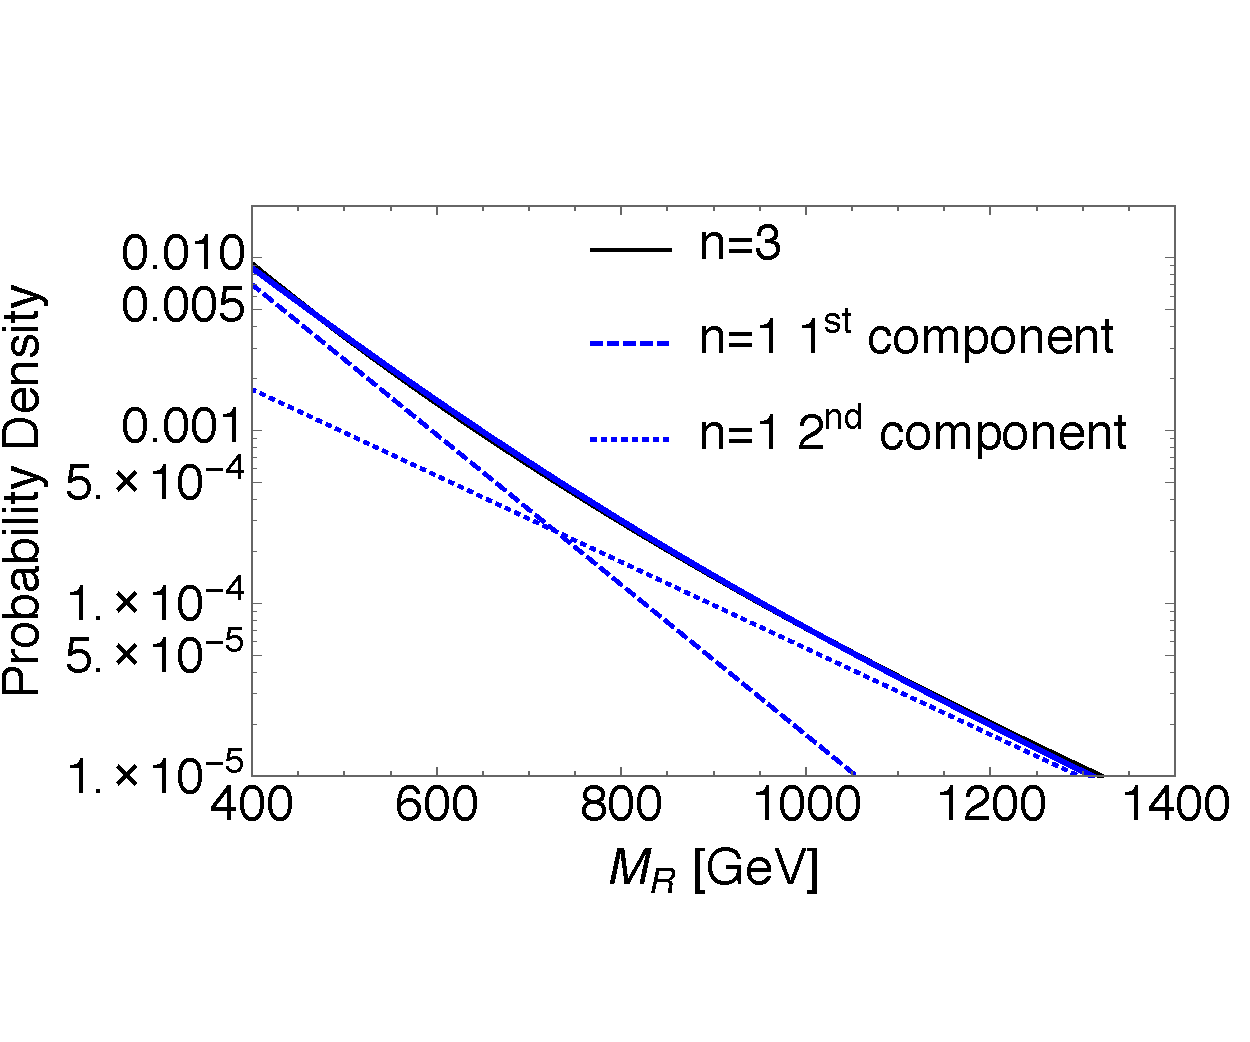
\includegraphics[width=0.8\textwidth,clip=true,viewport= 0 70 600 410]{figs/analysis8TeV/twoexp.pdf}
\caption{Two exponential components with $n=1$ and their sum are shown in blue compared with
  a single modified exponential with $n=3$ in black.\label{fig:twoexp}}
\end{figure}


One of the benefits of this functional form is that it is analytically
integrable. By providing the analytical integral to \textsc{RooFit},
we avoid using \textsc{RooFit}'s multi-dimensional numerical
integration, which is costly in terms of function evaluations and may be inaccurate~\cite{Anderson:2007}~\cite{Press:1992:NRC:148286}.
In particular, the one-dimensional and two-dimensional integrals of
the function are
\begin{align}
 \int^{\Rtwo_{\mathrm{max}}}_{\Rtwo_{\mathrm{min}}} f(\MR,\Rtwo)
  \mathrm{d}\Rtwo &=  
\exp\left(-bn(\MR-\MRz)^{1/n}(\Rtwo_{\mathrm{max}}-\Rtwoz)^{1/n}\right))~~~~~~~~~~~~~~~~~~~~\nonumber\\
&\times\exp\left(-bn(\MR-\MRz)^{1/n}(\Rtwo_{\mathrm{min}}-\Rtwoz)^{1/n}\right) \nonumber\\
&\times\bigg(\exp\left(-b n (\MR-\MRz)^{1/n}
   (\Rtwo_{\mathrm{max}}-\Rtwoz)^{1/n}\right) (\Rtwo_{\mathrm{min}}-\Rtwoz)\nonumber\\
& -\exp\left(-b n (\MR-\MRz)^{1/n} (\Rtwo_{\mathrm{min}}-\Rtwoz)^{1/n}\right)
   (\Rtwo_{\mathrm{max}}-\Rtwoz)\bigg)~,
\end{align}
and
\begin{align}
 \int^{\MR^{\mathrm{max}}}_{\MR^{\mathrm{min}}}
  \int^{\Rtwo_{\mathrm{max}}}_{\Rtwo_{\mathrm{min}}} f(\MR,\Rtwo)
  \mathrm{d}\Rtwo \mathrm{d}\MR &=  n (b n)^{-n} \bigg(\Gamma \left(n,b n (\MRz-\MR^{\mathrm{max}})^{1/n}
   (\Rtwoz-\Rtwo_{\mathrm{max}})^{1/n}\right)\nonumber\\
&- \Gamma \left(n,b n
   (\MR^{\mathrm{min}}-\MRz)^{1/n}
   (\Rtwo_{\mathrm{max}}-\Rtwoz)^{1/n}\right)\nonumber\\
&-\Gamma \left(n,b n
   (\MR^{\mathrm{max}}-\MRz)^{1/n}
   (\Rtwo_{\mathrm{min}}-\Rtwoz)^{1/n}\right)\nonumber\\
&+\Gamma \left(n,b n
   (\MR^{\mathrm{min}}-\MRz)^{1/n}
   (\Rtwo_{\mathrm{min}}-\Rtwoz)^{1/n}\right) \bigg)~,
\label{eq:razFunIntegrals}
\end{align}
respectively, where $\Gamma(a,x)$ is the incpmplete gamma function:
\begin{equation}
 \Gamma(a,x)=\int_{x}^{\infty}t^{a-1}e^{-t}\mathrm{d}t~.
\end{equation}

The shape of the empirical function is determined through a \textsc{RooFit}-based extended and unbinned
maximum likelihood fit to the data~\cite{Verkerke:2003ir}. Two kinds
of fit are performed: (i)~a sideband-only fit, which is extrapolated
to the signal region in order to test for the presence of a signal
(discussed in the remainder of this section), and (ii)~a simultaneous
fit to the signal and sideband regions, performed both under the
background-only and background-plus-signal hypotheses, which is used
for the interpretation of the results (Section~\ref{sec:limit}). In both cases, the empirical function is
found to adequately describe the SM background in each of the boxes,
for each \PQb-tagged jet multiplicity value.

The SM background-only likelihood function for the two-lepton boxes is written as:
\begin{equation}
\mathcal{L}(\text{data}|\boldsymbol\theta) = \frac{\re^{-N_\mathrm{SM}}}{N!} \prod_{i=1}^{N} N_\mathrm{SM}
 P_\mathrm{SM}({\MR}_{(i)},{\Rtwo}_{(i)}),
\label{eq:Lik1btag}
\end{equation}
where $P_\mathrm{SM}(\MR,\Rtwo)$ is the empirical function in
Eq.~(\ref{eq:razFun}) normalized to unity, $N_{SM}$ is the
corresponding normalization factor, $\boldsymbol\theta$ is the set of
background shape and normalization parameters, and the product runs
over the $N$ events in the data set. The same form of the
likelihood is used for the other boxes, for each \PQb-tagged jet
multiplicity. The total likelihood in these boxes is computed as the
product of the likelihood functions for each \PQb-tagged jet
multiplicity.

The fits are performed independently for each box and simultaneously
across the \PQb-tagged jet multiplicity bins. Common background shape
parameters ($b$, ${\MR}^0$, $\Rtwoz$, and $n$) are used
for the 2 \PQb-tag and $\geq$3 \PQb-tag bins, since no substantial
difference between the two distributions is observed on large samples
of $\ttbar$ and $\cPV$+jets MC events. A difference is observed
between 1 \PQb-tag and $\geq$2 \PQb-tag samples, due to the observed
dependence of the \PQb-tagging efficiency on the jet $\pt$. Consequently,
the shape parameters for the 1 \PQb-tag bins are allowed to differ
from the corresponding parameters for the $\geq$2 \PQb-tag bins. The
background normalization parameters for each \PQb-tagged jet multiplicity
bin are also treated as independent parameters.

The background shape parameters are estimated from the events in the
two sidebands (Section~\ref{sec:razVar}). This shape is then used to
derive a background prediction in the signal-sensitive region:
$30\,000$ alternative sets of background shape parameters are generated
from the covariance matrix returned by the fit. An ensemble of
pseudo-experiment data sets is created, generating random
($\MR$, $\Rtwo$) pairs distributed according to each
of these alternative shapes. For each bin of the signal-sensitive
region, the distribution of the predicted yields in each
pseudo-experiment is compared to the observed yield in data in order
to quantify the agreement between the background model and the
observation. The agreement, described as a two-sided p-value, is then
translated into the corresponding number of standard deviations for a
normal distribution. The p-value is computed using the probability
density as the ordering principle. The observed numbers of standard
deviations in the two-lepton boxes are shown in
Fig.~\ref{fig:FrenchFlagDilep}, as a function of \MR and
$\Rtwo$. Positive and negative significance correspond to
regions where the observed yield is respectively larger and smaller
than the predicted one. Light gray areas correspond to empty bins with
less than one event expected on average. Similar results for the
one-lepton and hadronic boxes are shown in
Figs.~\ref{fig:FrenchFlagLep} and
\ref{fig:FrenchFlagHad}. Figures~\ref{fig:Proj1DDilep}--\ref{fig:Proj1DHad}
illustrate the extrapolation of the fit results to the full
($\MR$, $\Rtwo$) plane, projected onto  \Rtwo and \MR and summed over the \PQb-tagged jet multiplicity
bins. No significant deviation of data from the SM background
predictions is observed.

\begin{figure}[tb!]
\centering
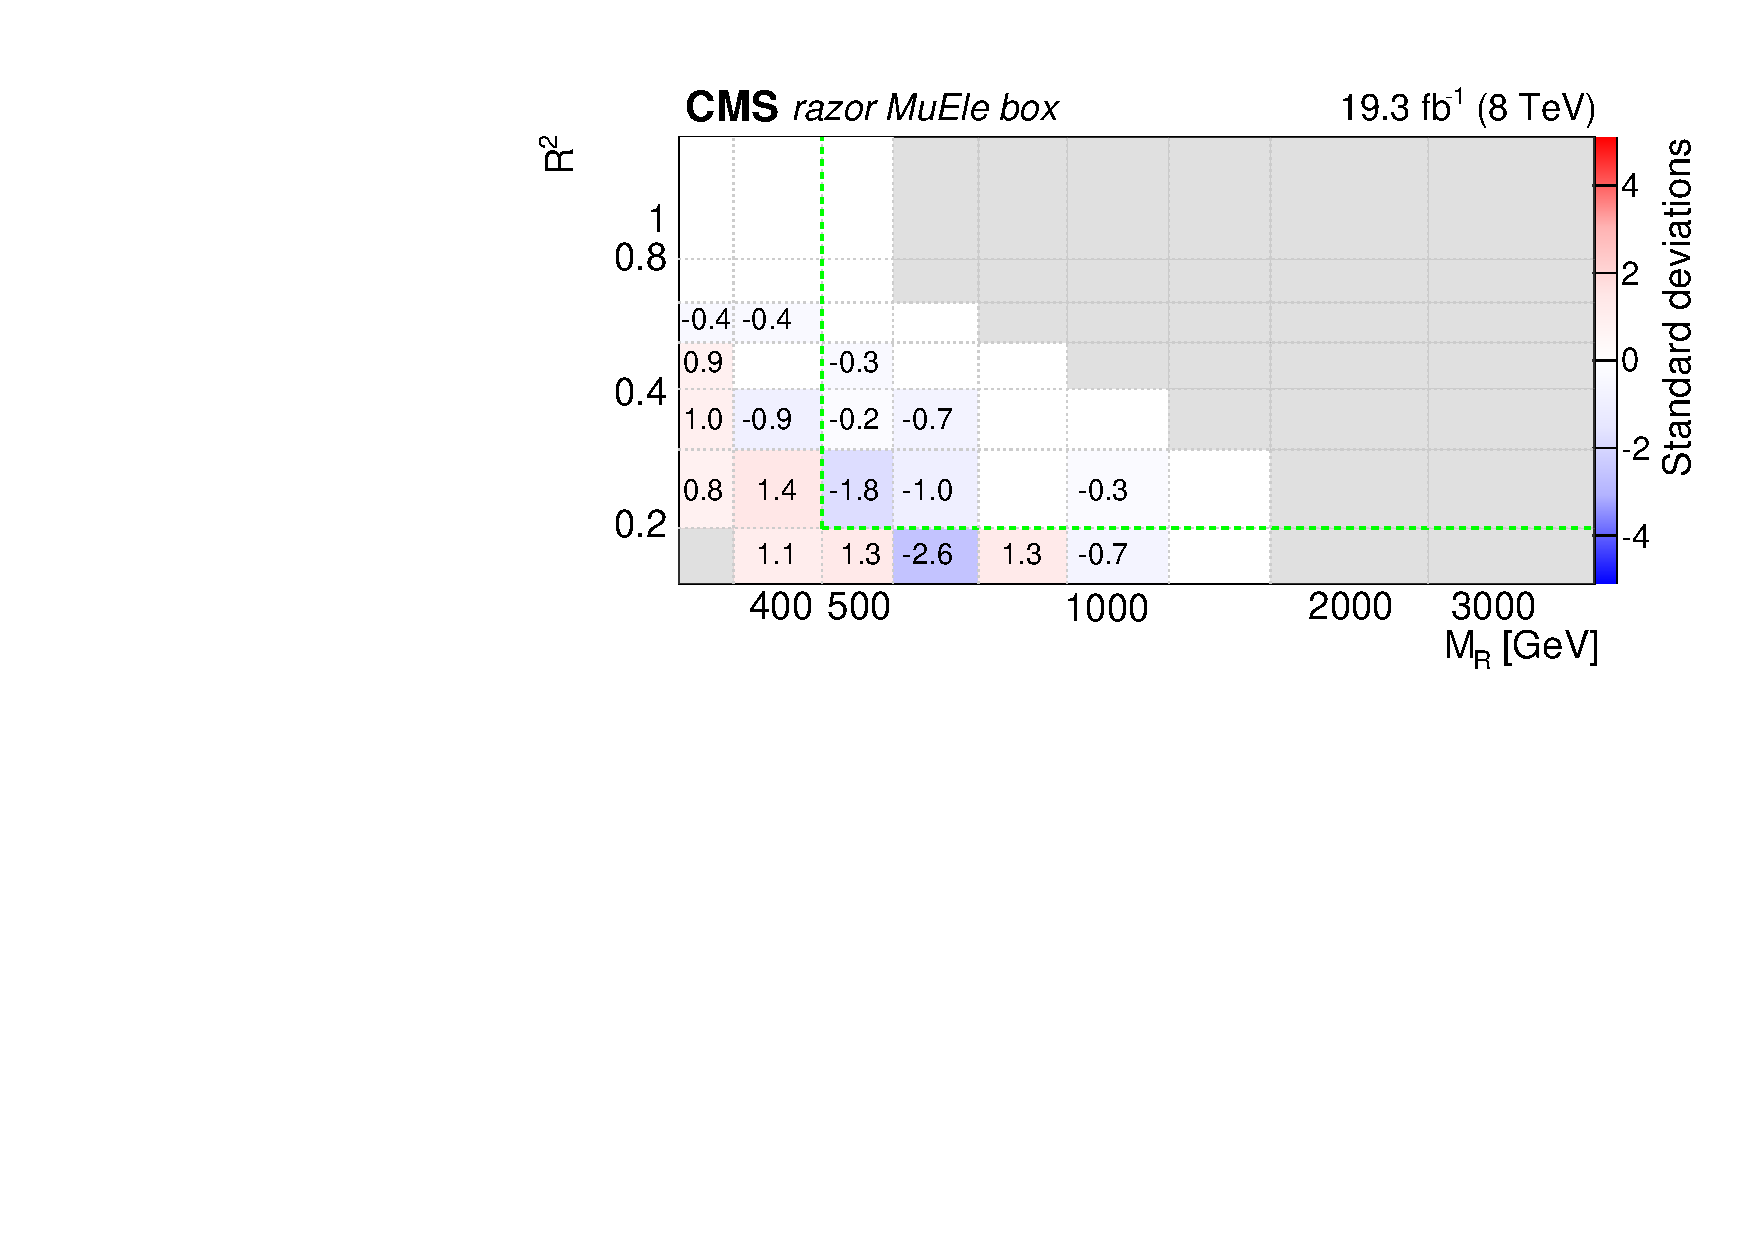
\includegraphics[width=0.49\textwidth]{figs/analysis8TeV/nSigmaLog_MuEle.pdf}
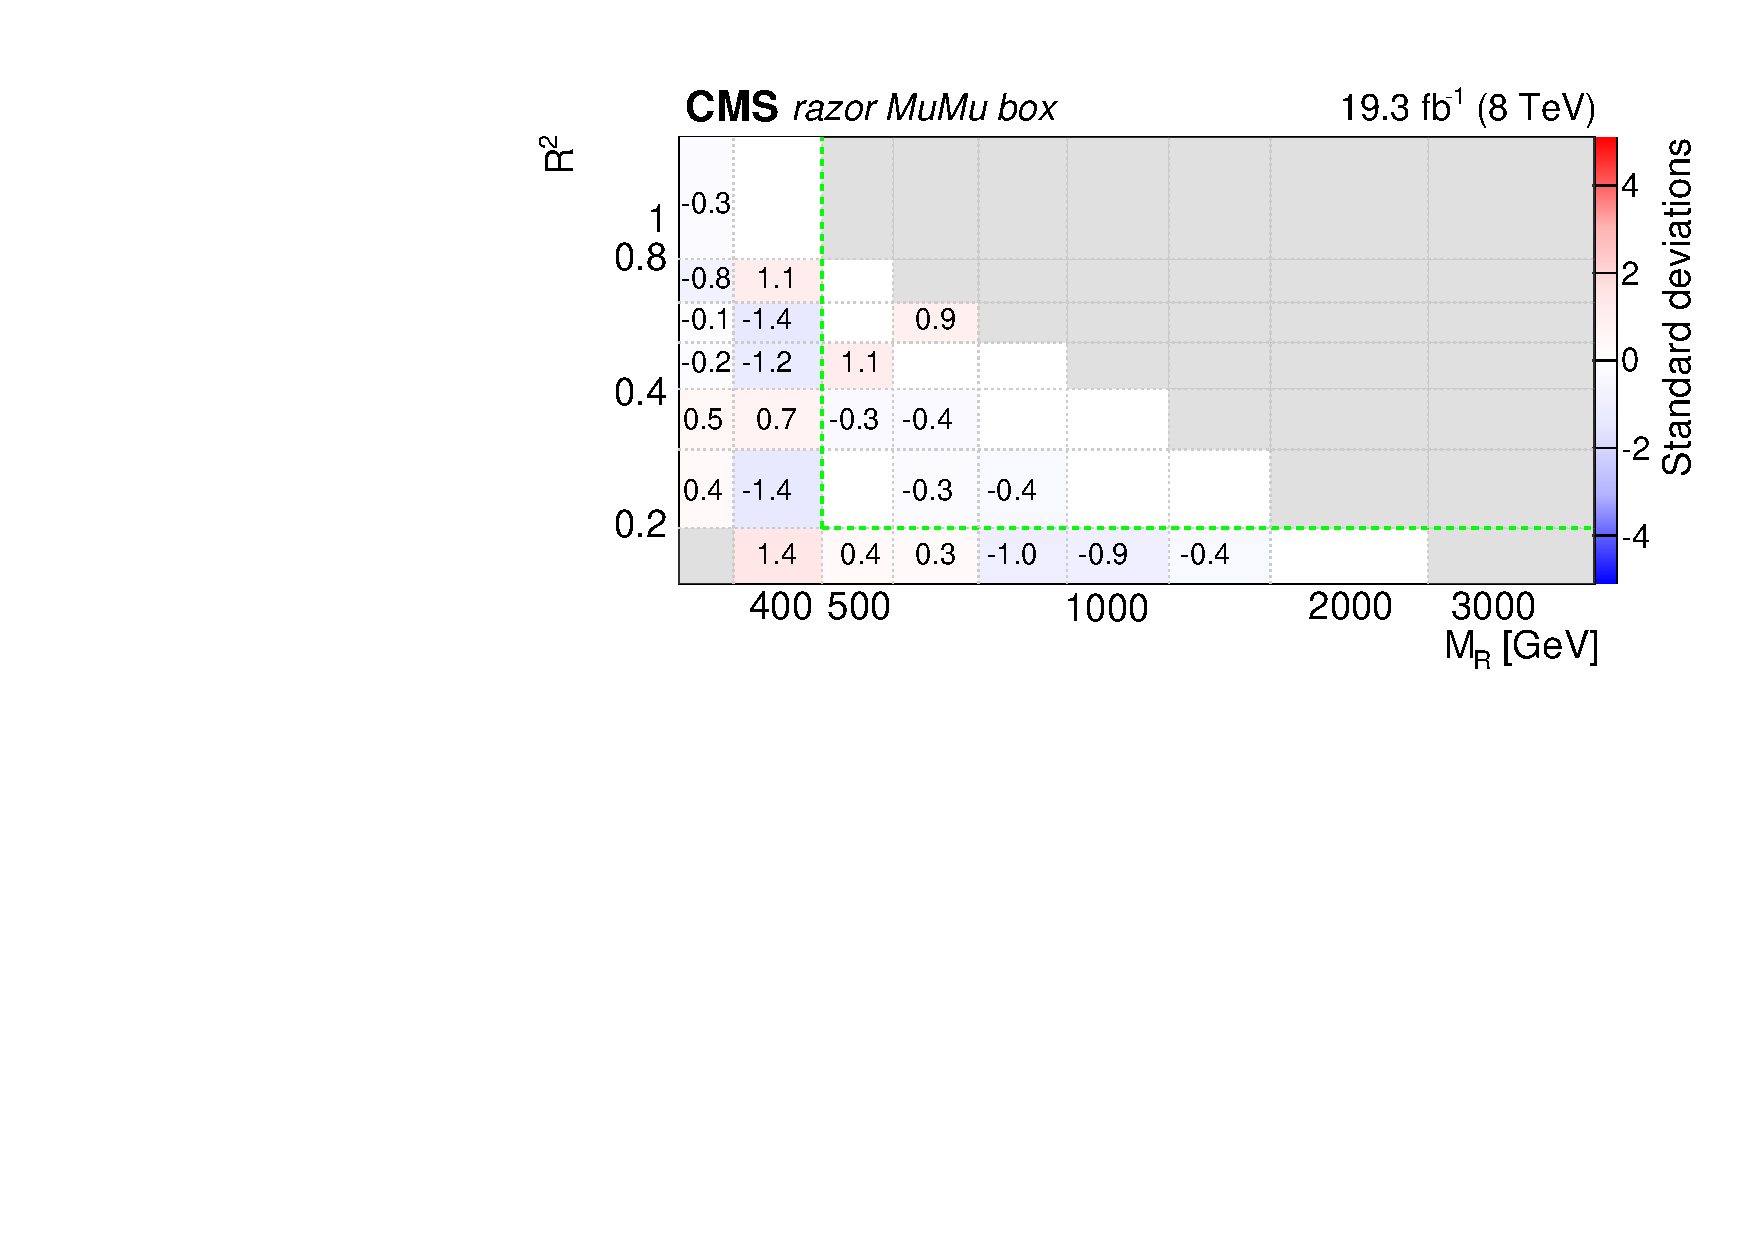
\includegraphics[width=0.49\textwidth]{figs/analysis8TeV/nSigmaLog_MuMu.pdf}
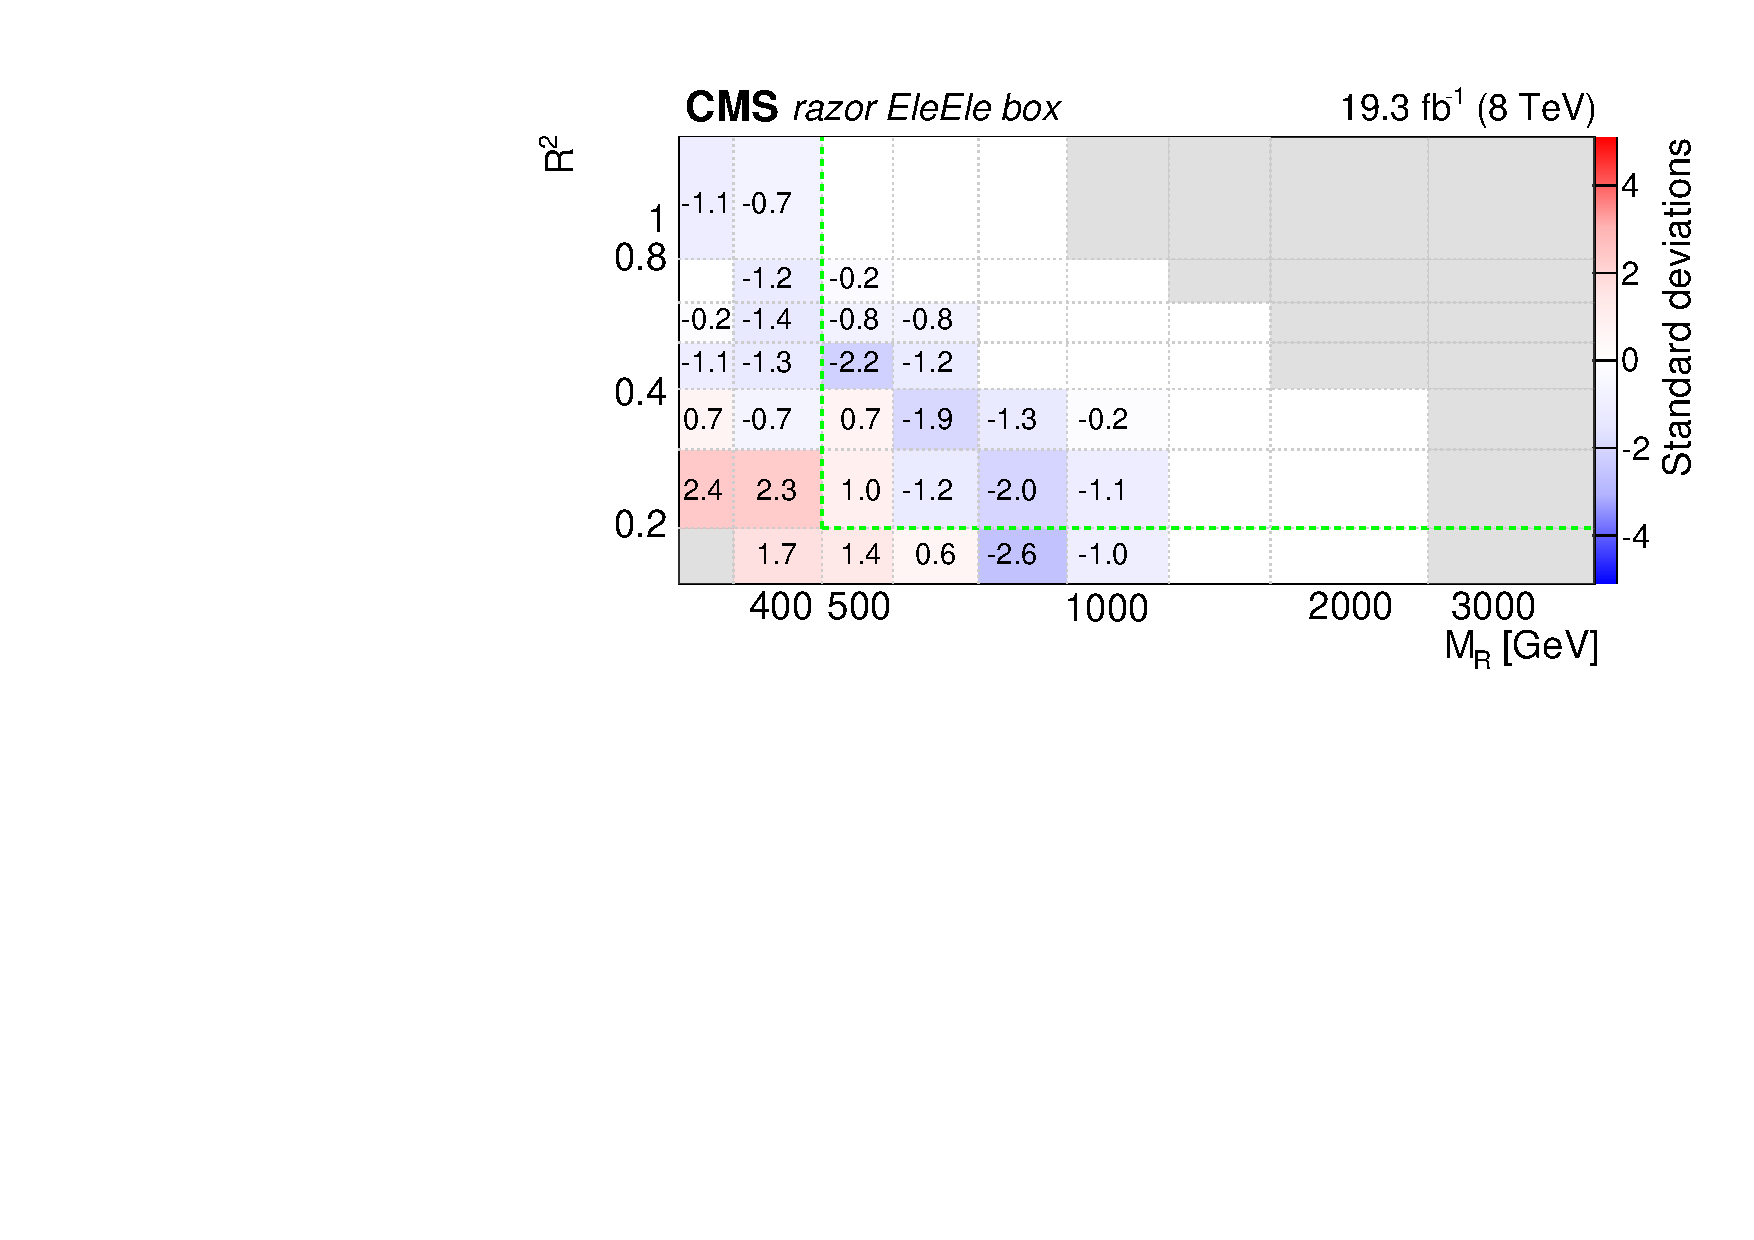
\includegraphics[width=0.49\textwidth]{figs/analysis8TeV/nSigmaLog_EleEle.pdf}
\caption{Comparison of the expected background and the observed yield
  in the (upper left) MuEle, (upper right) MuMu, and (bottom)
  EleEle boxes. A probability density function is derived for the
  bin-by-bin yield using pseudo-experiments, sampled from the output
  of the corresponding sideband fit. A two sided p-value is computed
  comparing the observed yield to the distribution of background yield
  from pseudo-experiments. The p-value is translated into the
  corresponding number of standard deviations, quoted in each bin and
  represented by the bin-filling color. Positive and negative
  significance correspond to regions where the observed yield is
  respectively larger and smaller than the predicted one. The white areas
  correspond to bins in which a difference smaller than 0.1 standard
  deviations is observed. The gray areas correspond to empty bins with
  less than one background event expected on average. The dashed lines
  represent the boundaries between the sideband and the signal
  regions.\label{fig:FrenchFlagDilep}}

\end{figure}

\begin{figure*}[tb!]
\centering
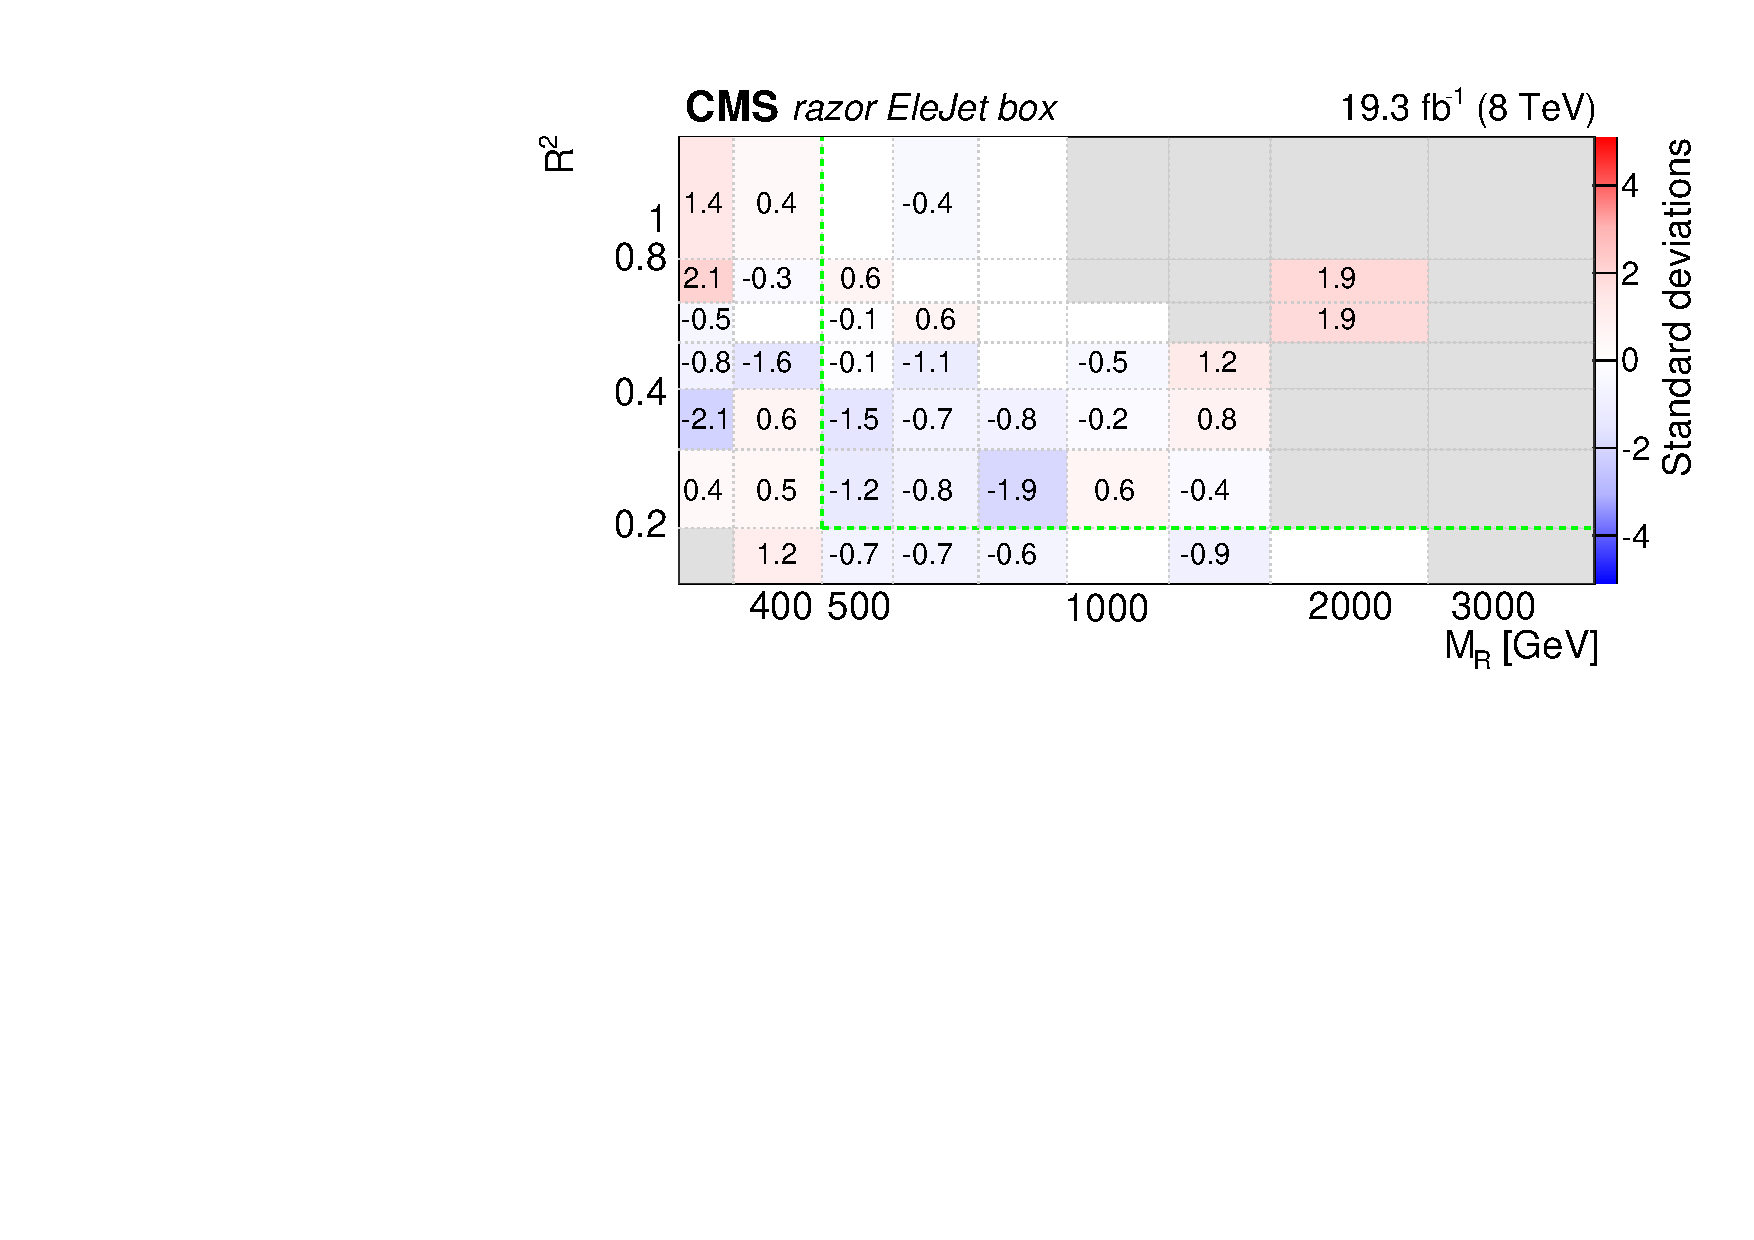
\includegraphics[width=0.49\textwidth]{figs/analysis8TeV/nSigmaLog_EleJet.pdf}
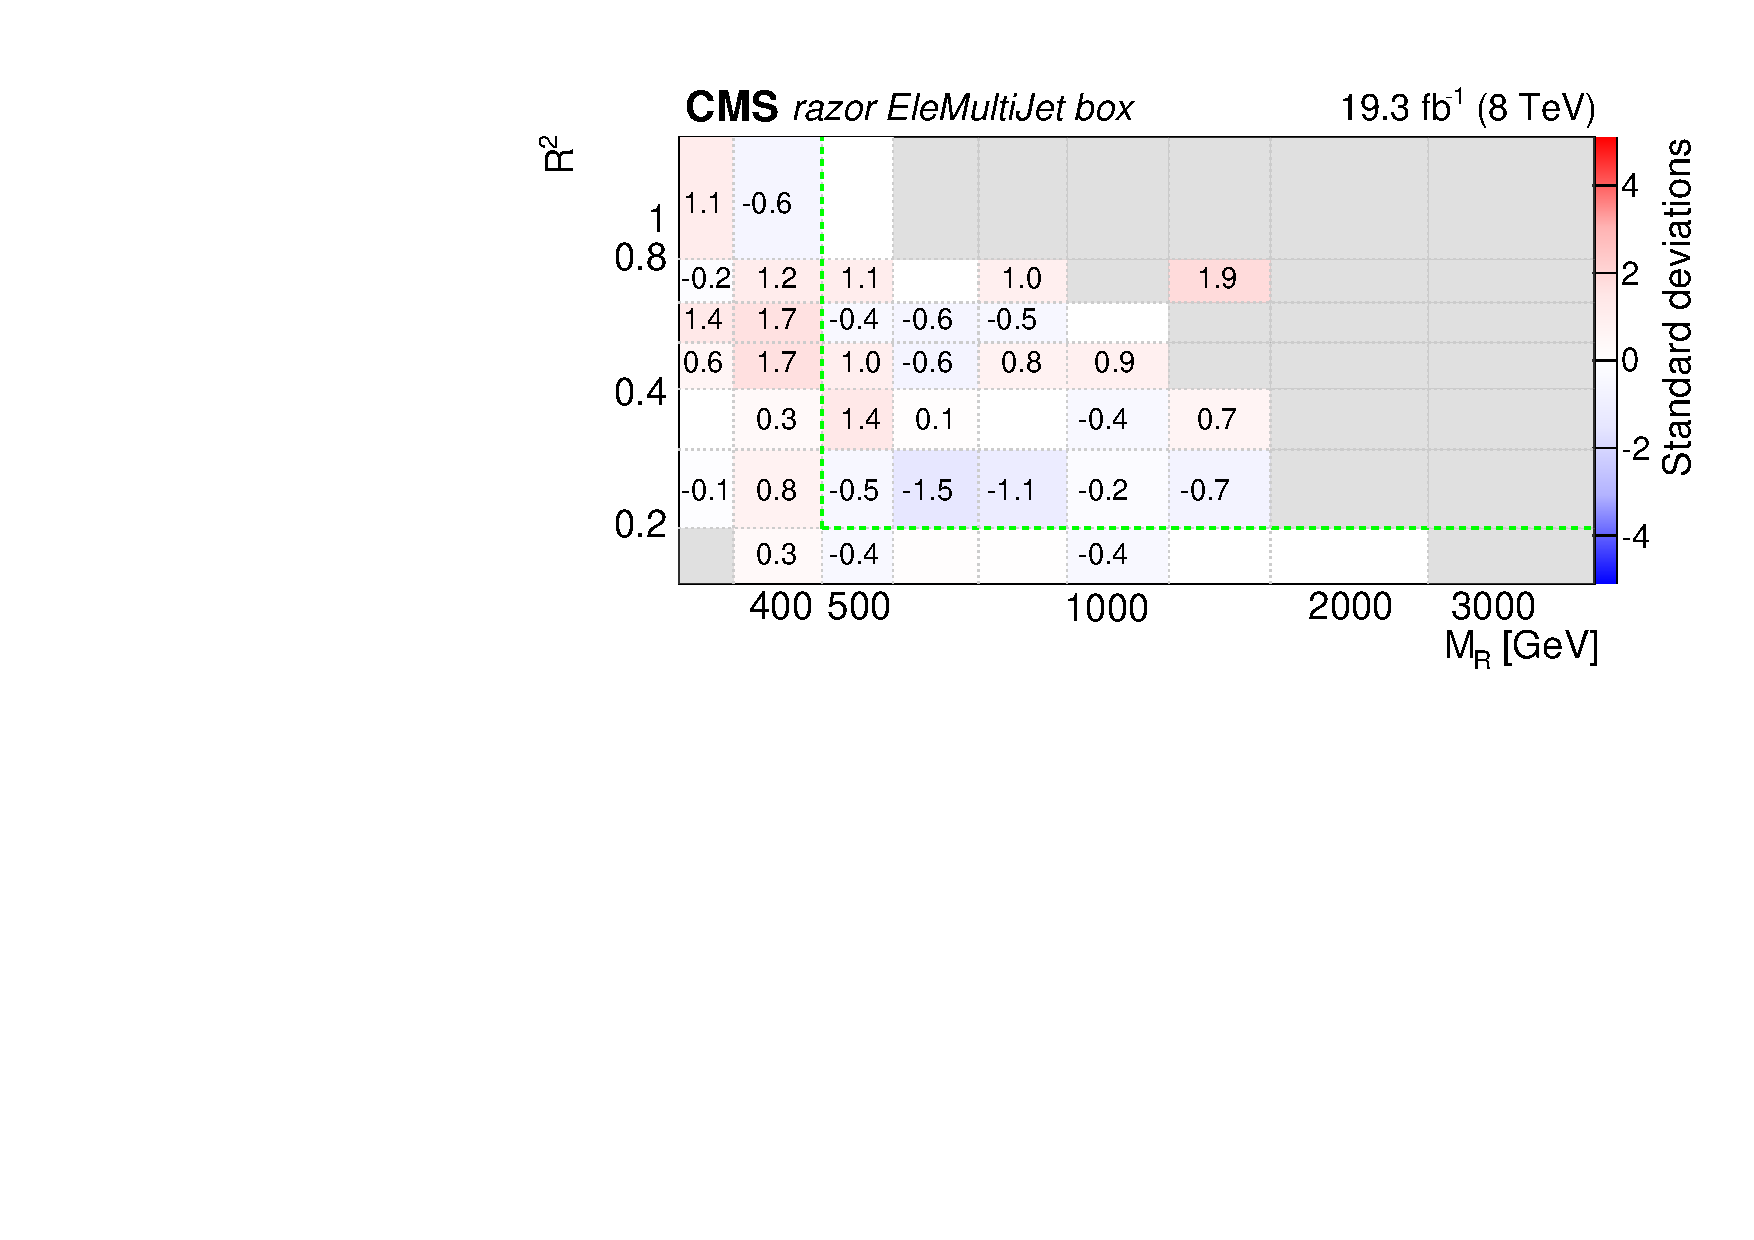
\includegraphics[width=0.49\textwidth]{figs/analysis8TeV/nSigmaLog_EleMultiJet.pdf}
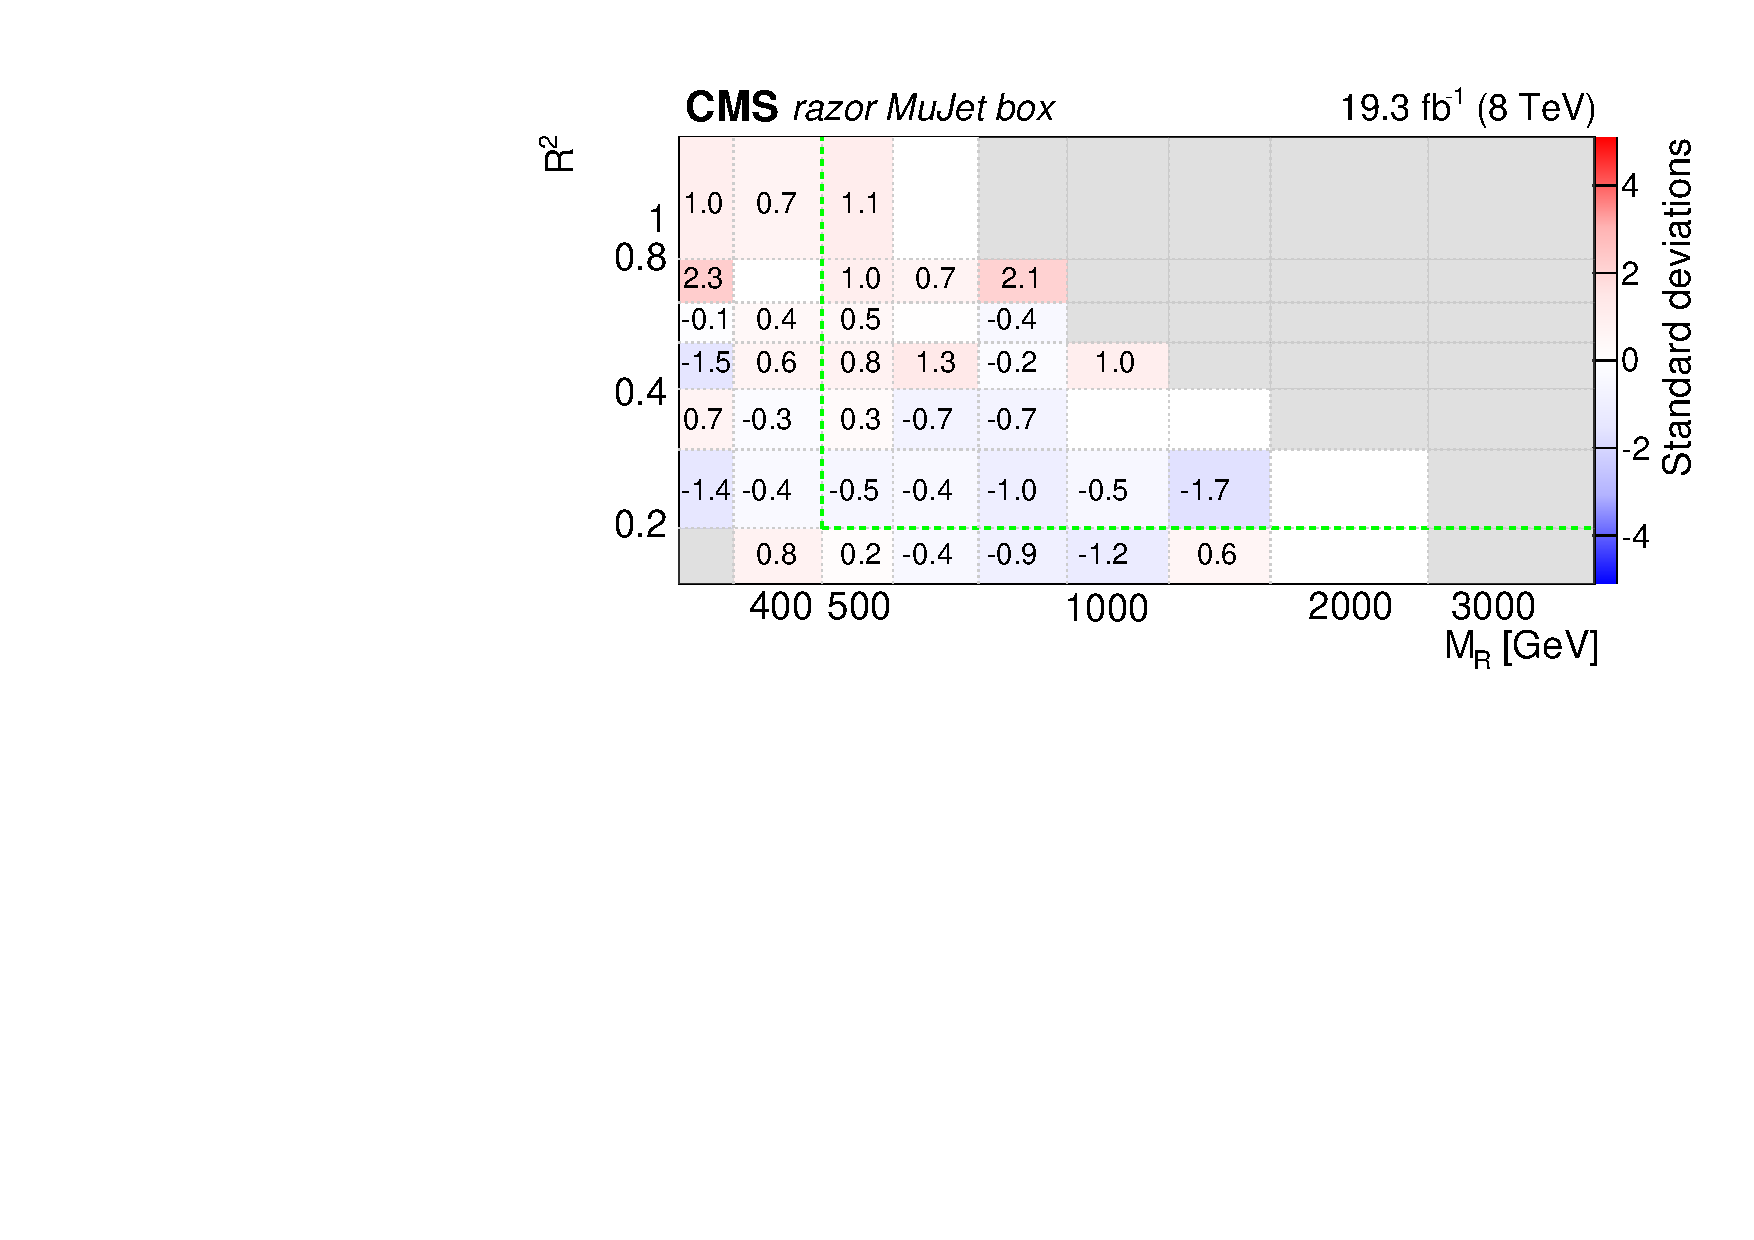
\includegraphics[width=0.49\textwidth]{figs/analysis8TeV/nSigmaLog_MuJet.pdf}
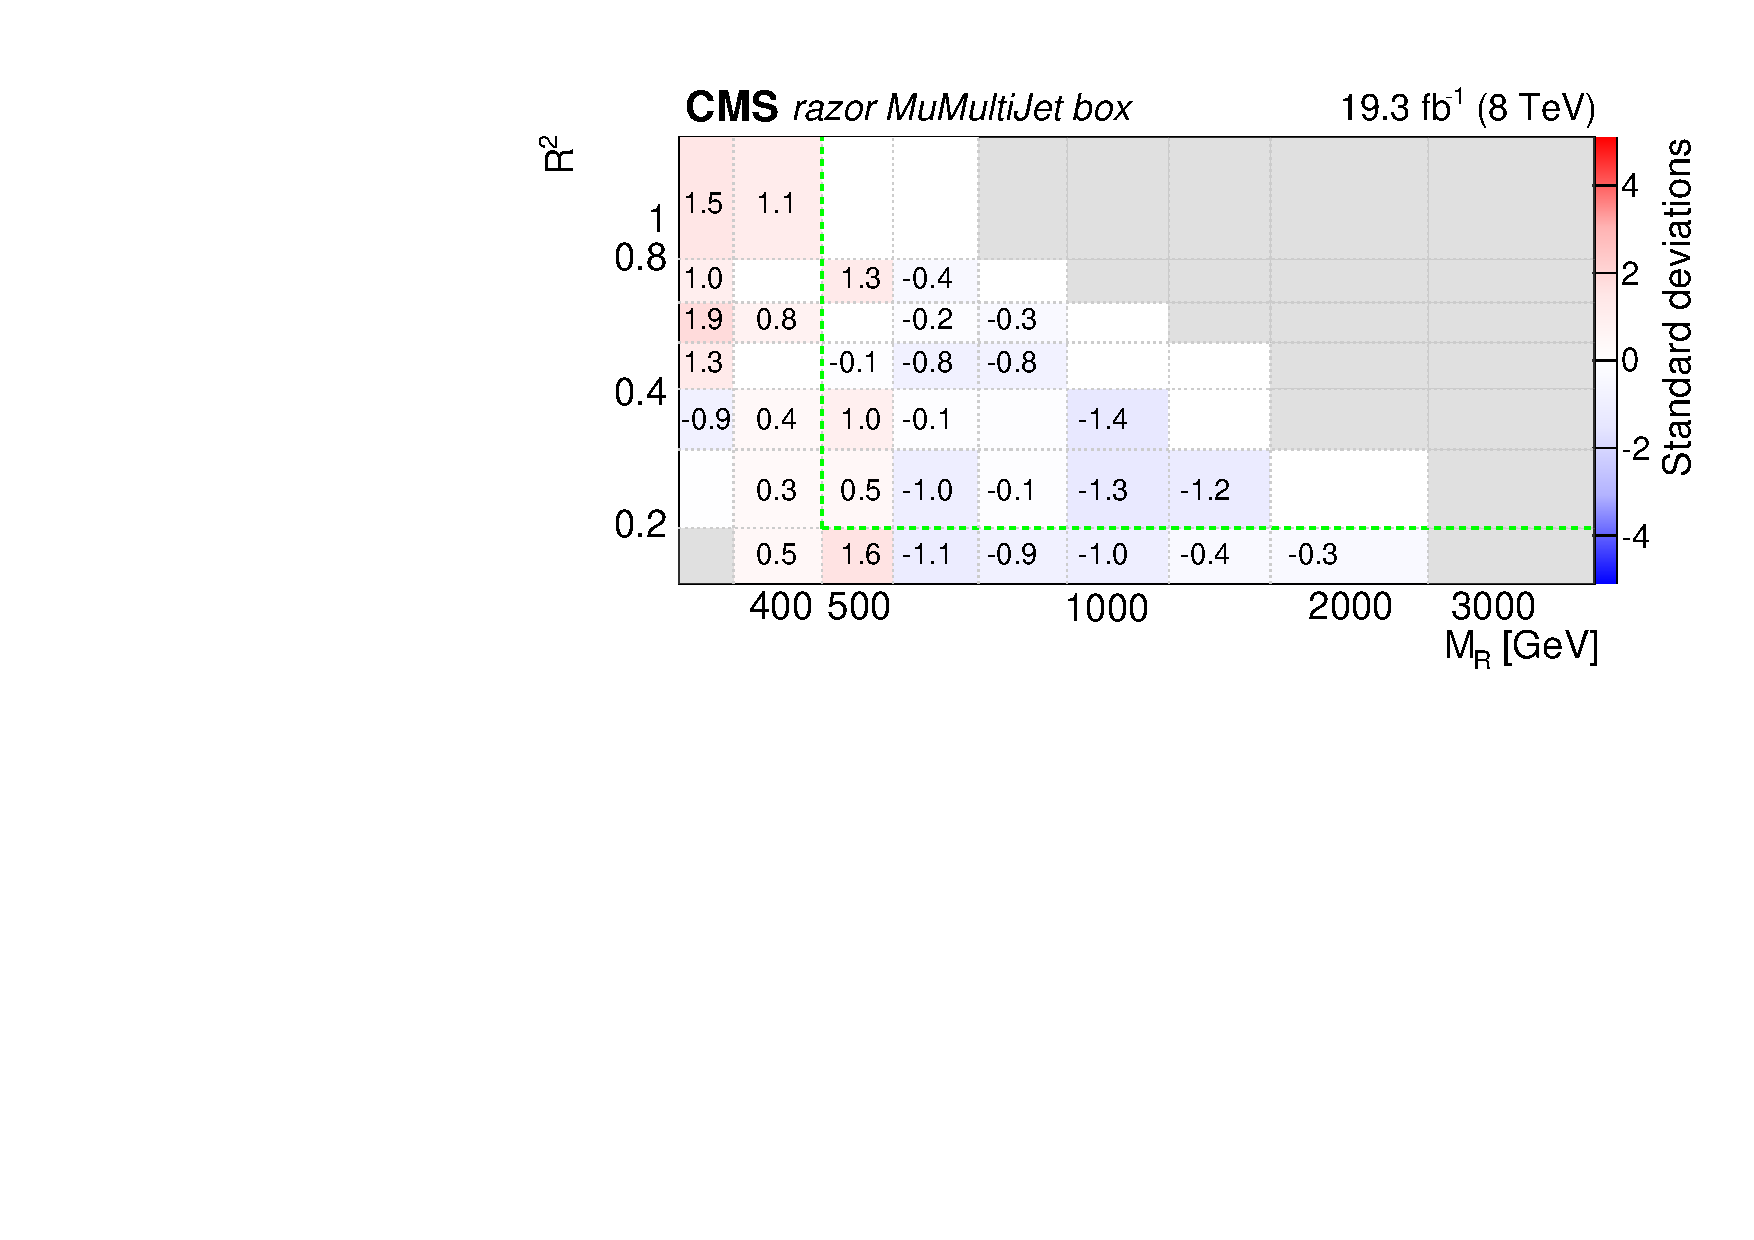
\includegraphics[width=0.49\textwidth]{figs/analysis8TeV/nSigmaLog_MuMultiJet.pdf}
\caption{Comparison of the expected background and the observed yield
  in (upper left) the EleJet, (upper right) the EleMultiJet, (lower left) the MuJet, and (lower right) the MuMultiJet
  boxes. A detailed explanation is given in the caption of
  Fig.~\ref{fig:FrenchFlagDilep}.\label{fig:FrenchFlagLep}}
\end{figure*}

\begin{figure}[tb!]
\centering
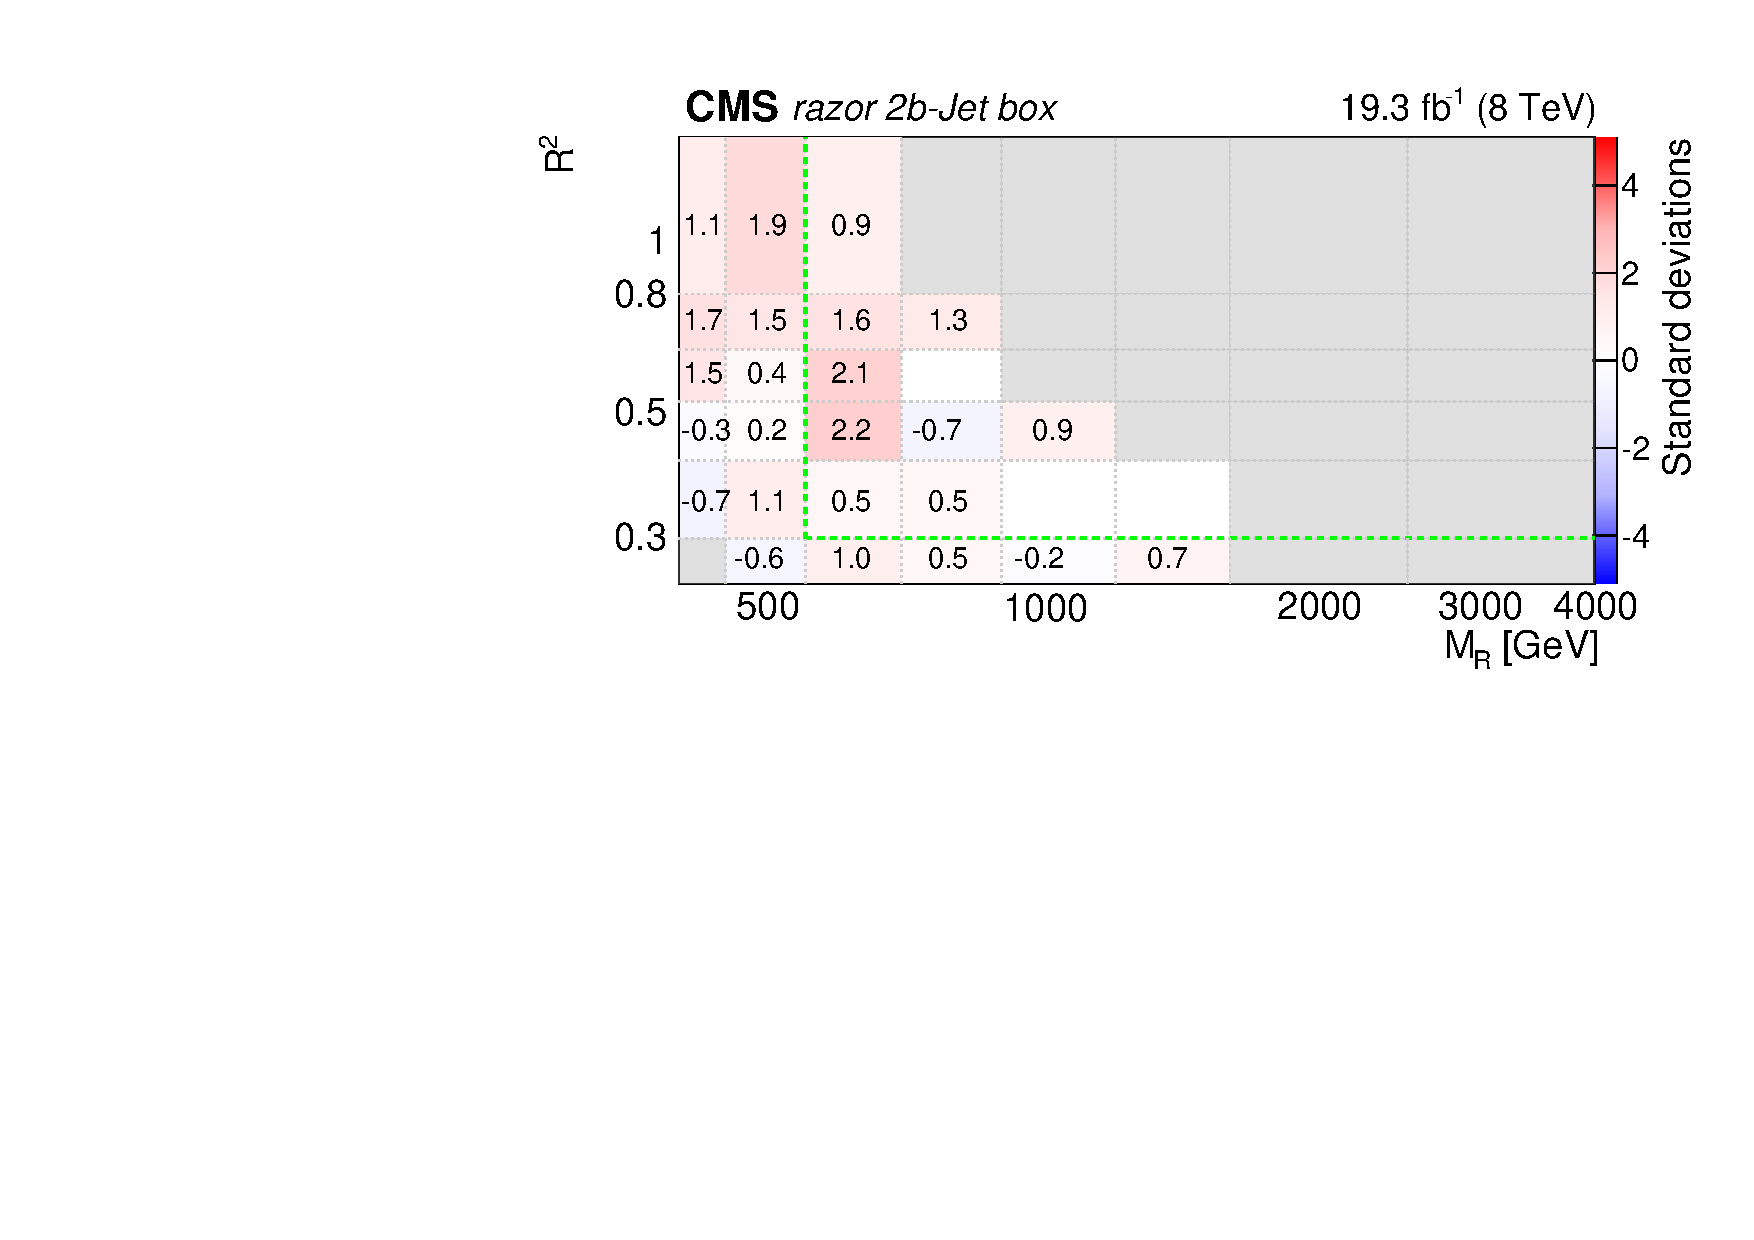
\includegraphics[width=0.49\textwidth]{figs/analysis8TeV/nSigmaLog_Jet2b.pdf}
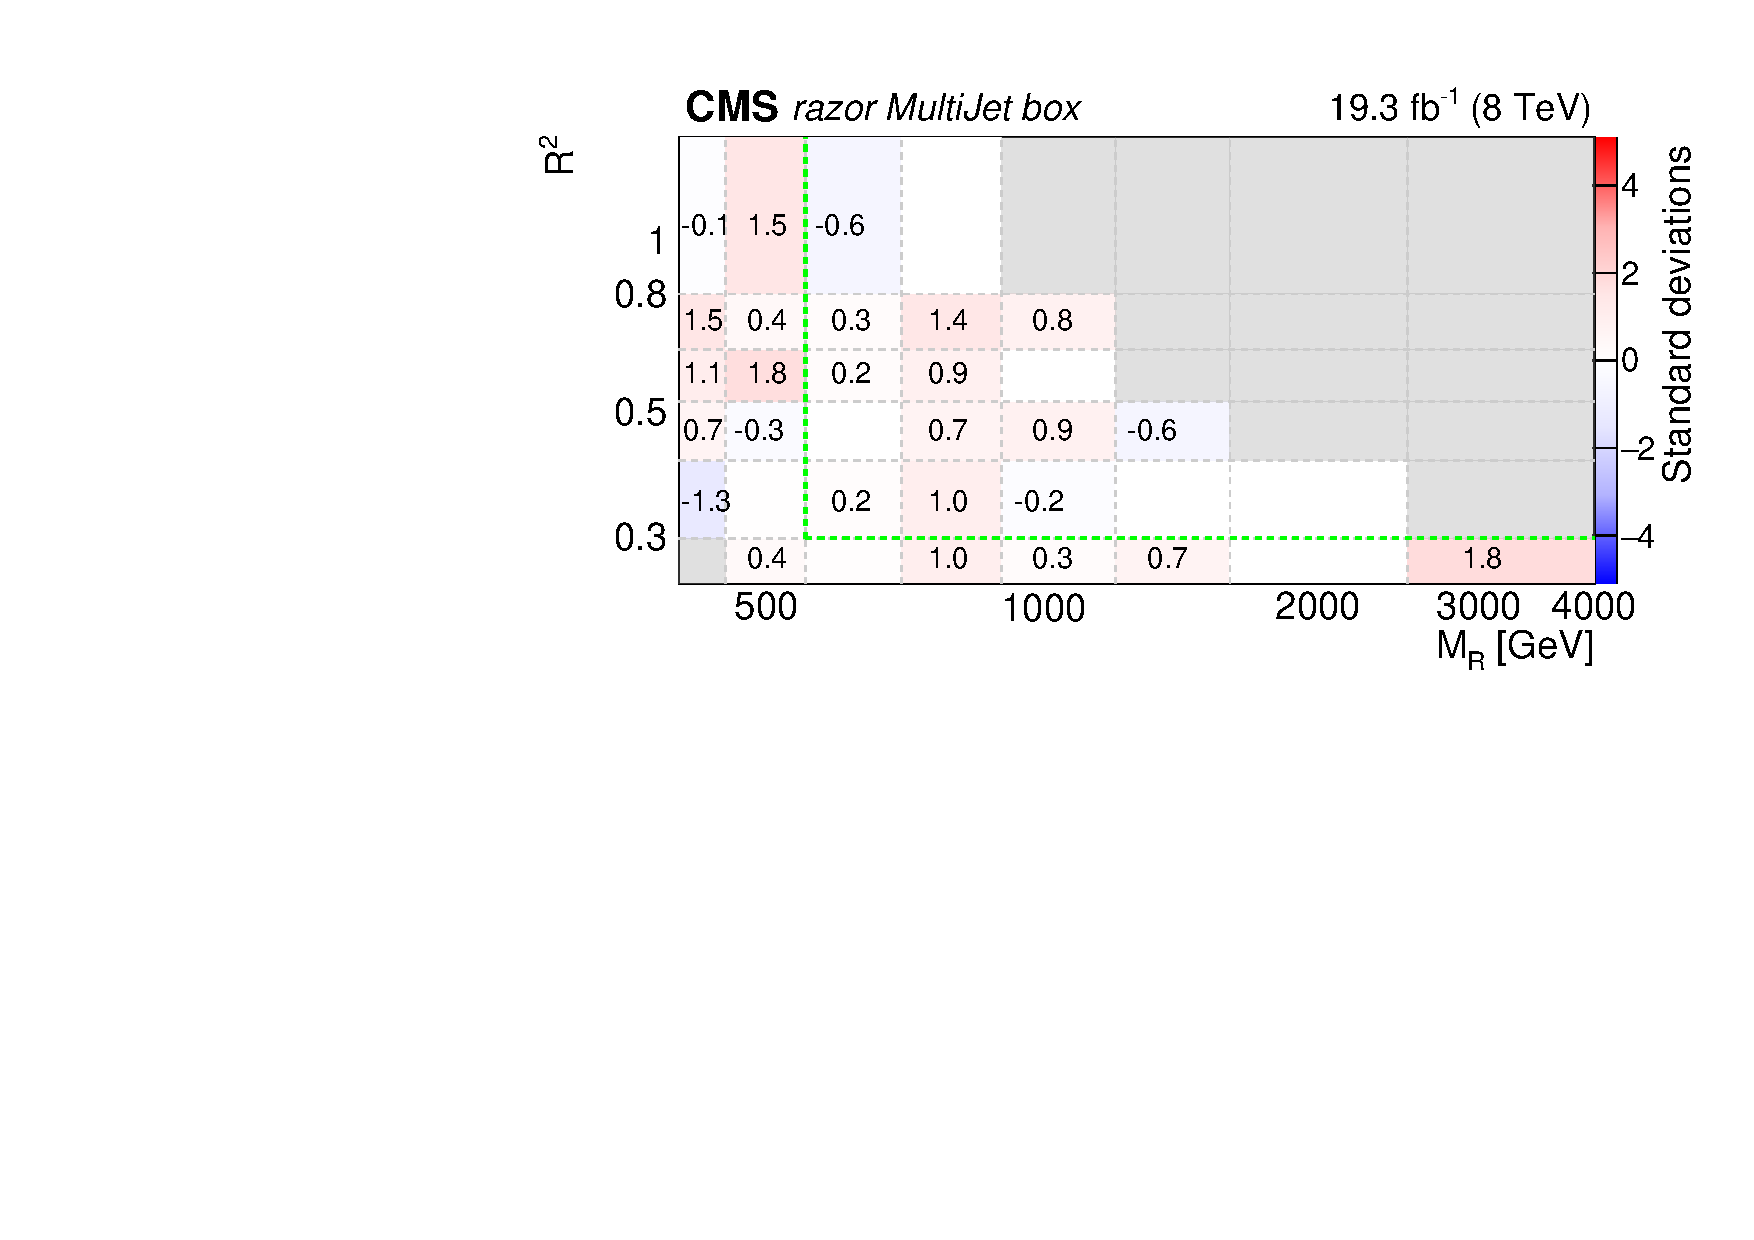
\includegraphics[width=0.49\textwidth]{figs/analysis8TeV/nSigmaLog_MultiJetFITS.pdf}
\caption{Comparison of the expected background and the observed yield
  in the $\geq$2 \PQb-tagged jet box (left) and the MultiJet box
  (right). A detailed explanation is given in the caption of
  Fig.~\ref{fig:FrenchFlagDilep}.\label{fig:FrenchFlagHad}}

\end{figure}

\begin{figure*}[tb!]
\centering
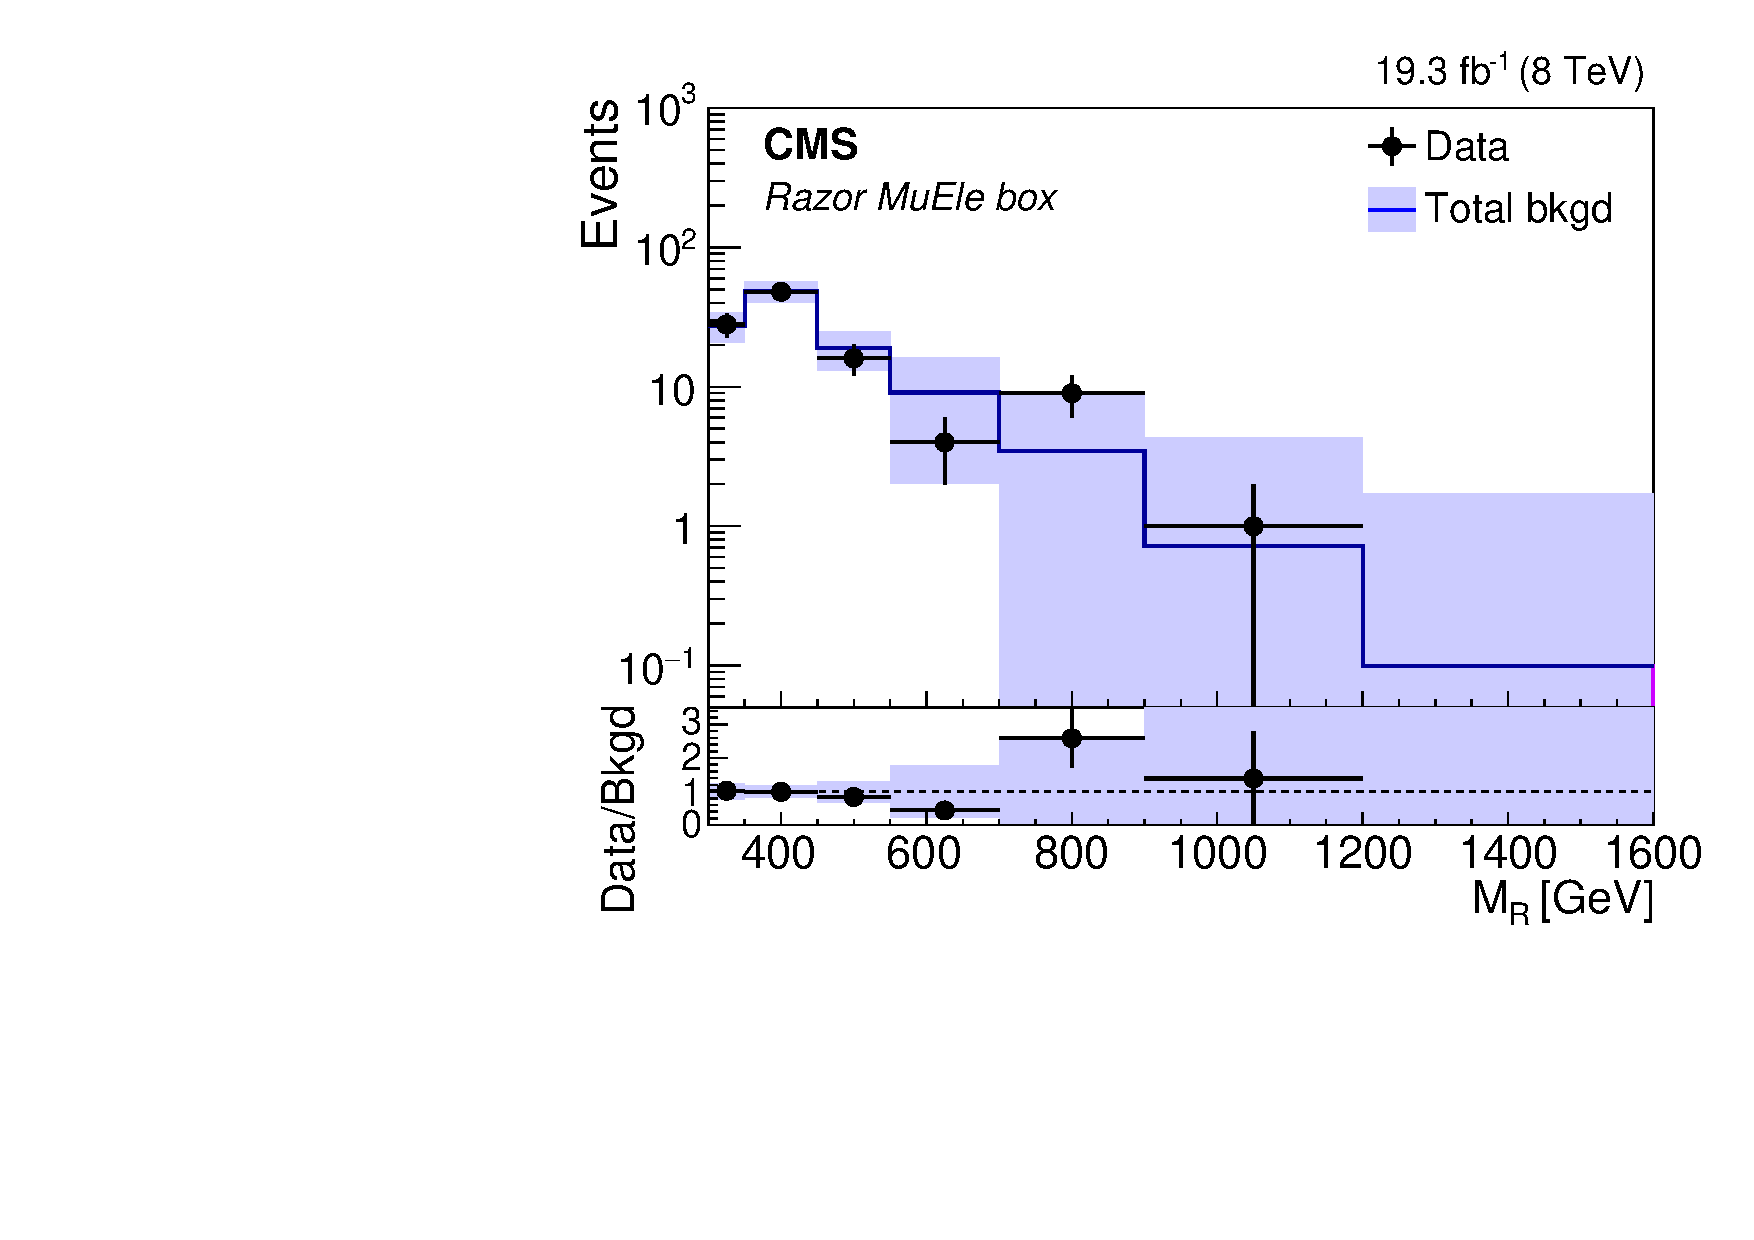
\includegraphics[width=0.49\textwidth]{figs/analysis8TeV/MR_ElectronHad-Run2012ABCD_Sideband_MuEle.pdf}
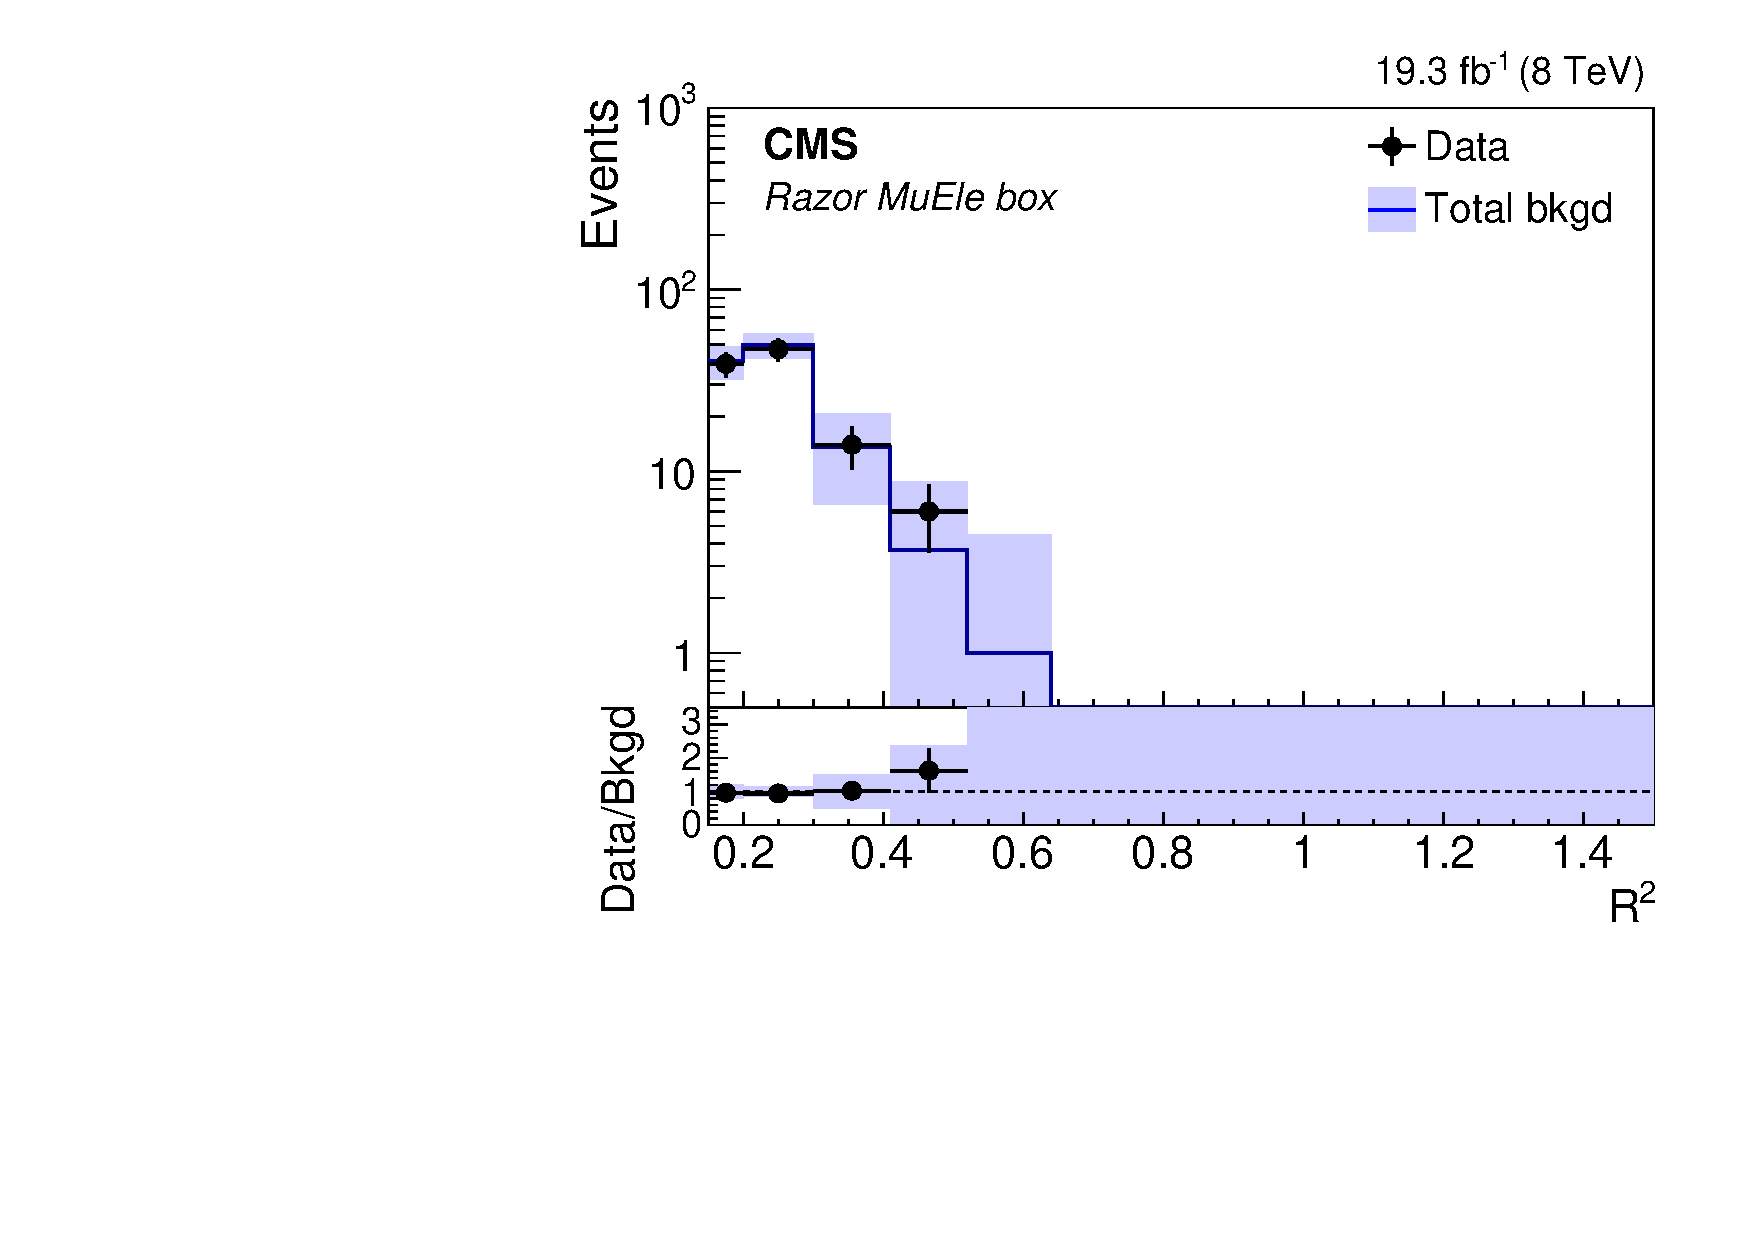
\includegraphics[width=0.49\textwidth]{figs/analysis8TeV/RSQ_ElectronHad-Run2012ABCD_Sideband_MuEle.pdf}
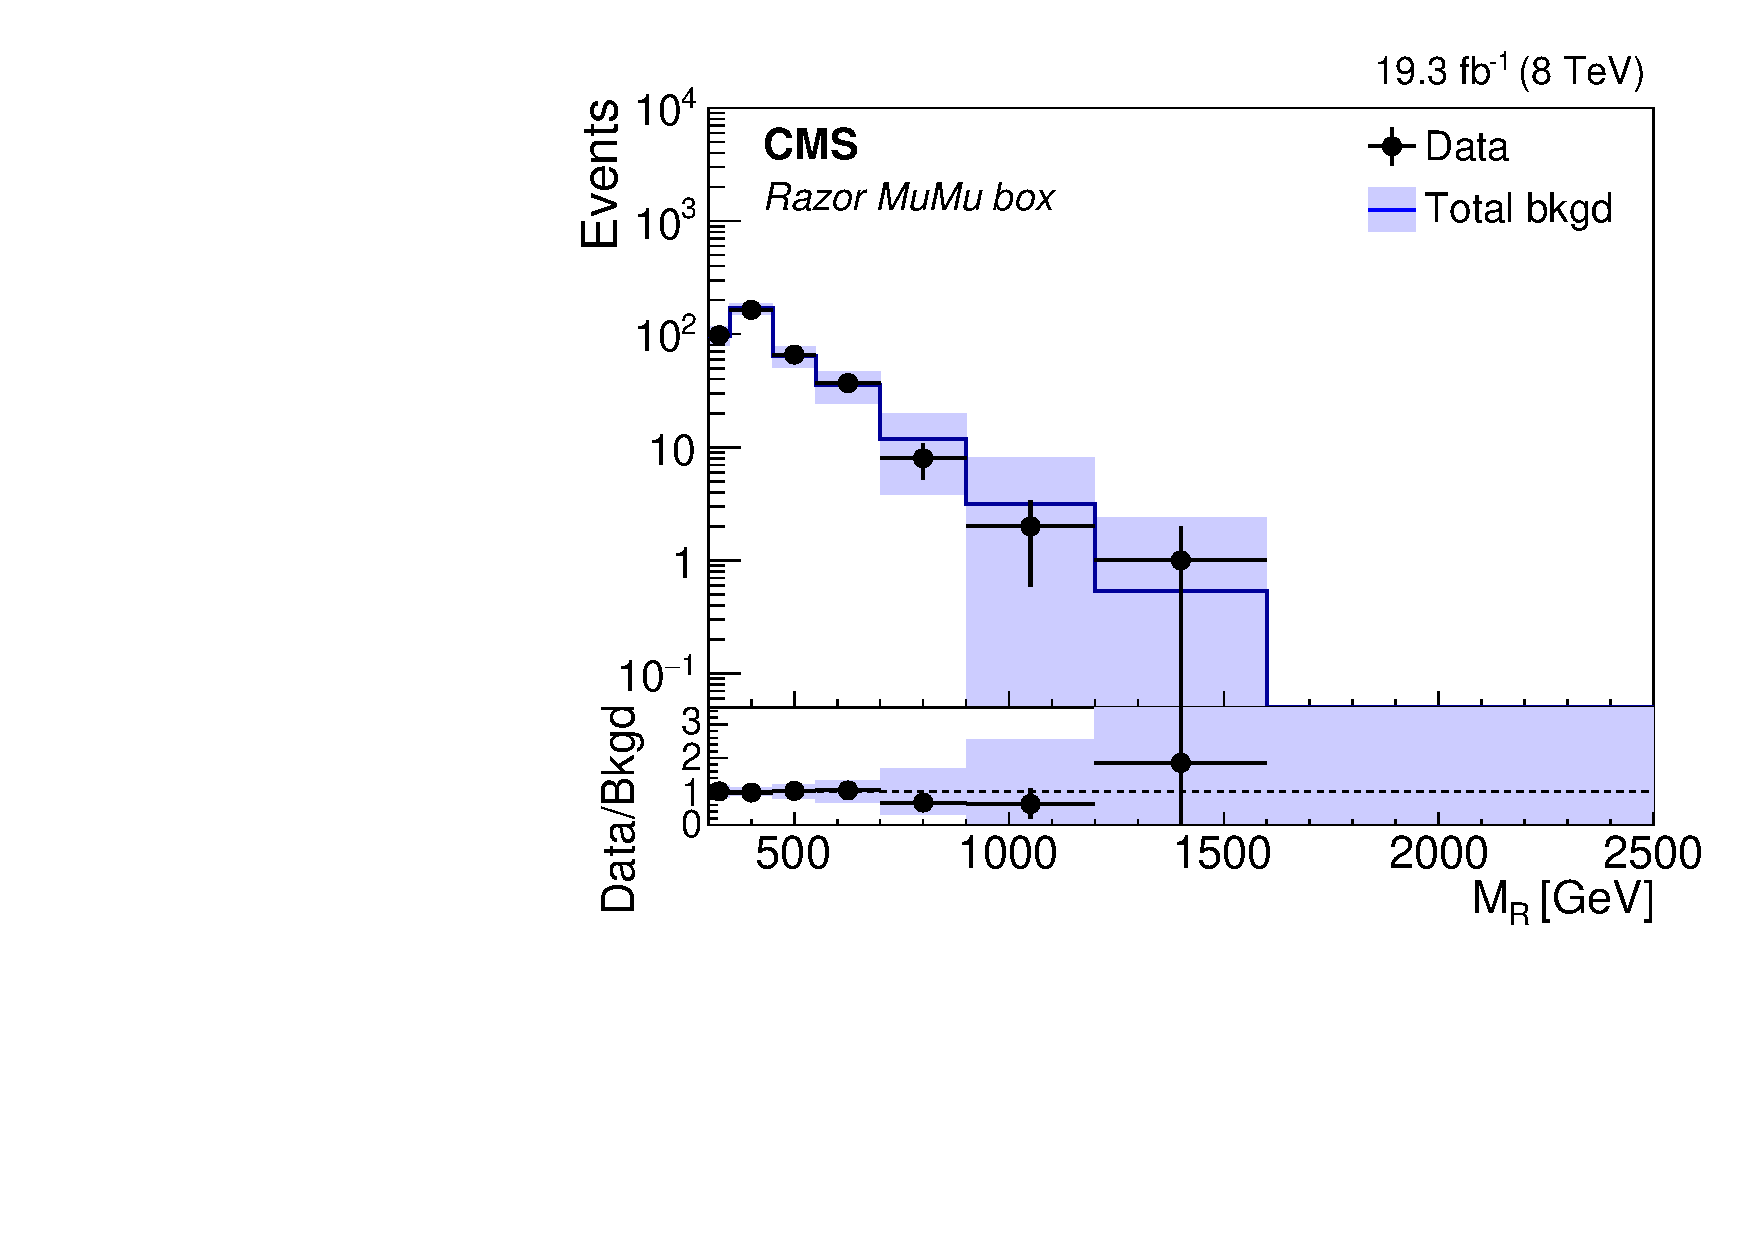
\includegraphics[width=0.49\textwidth]{figs/analysis8TeV/MR_MuHad-Run2012ABCD_Sideband_MuMu.pdf}
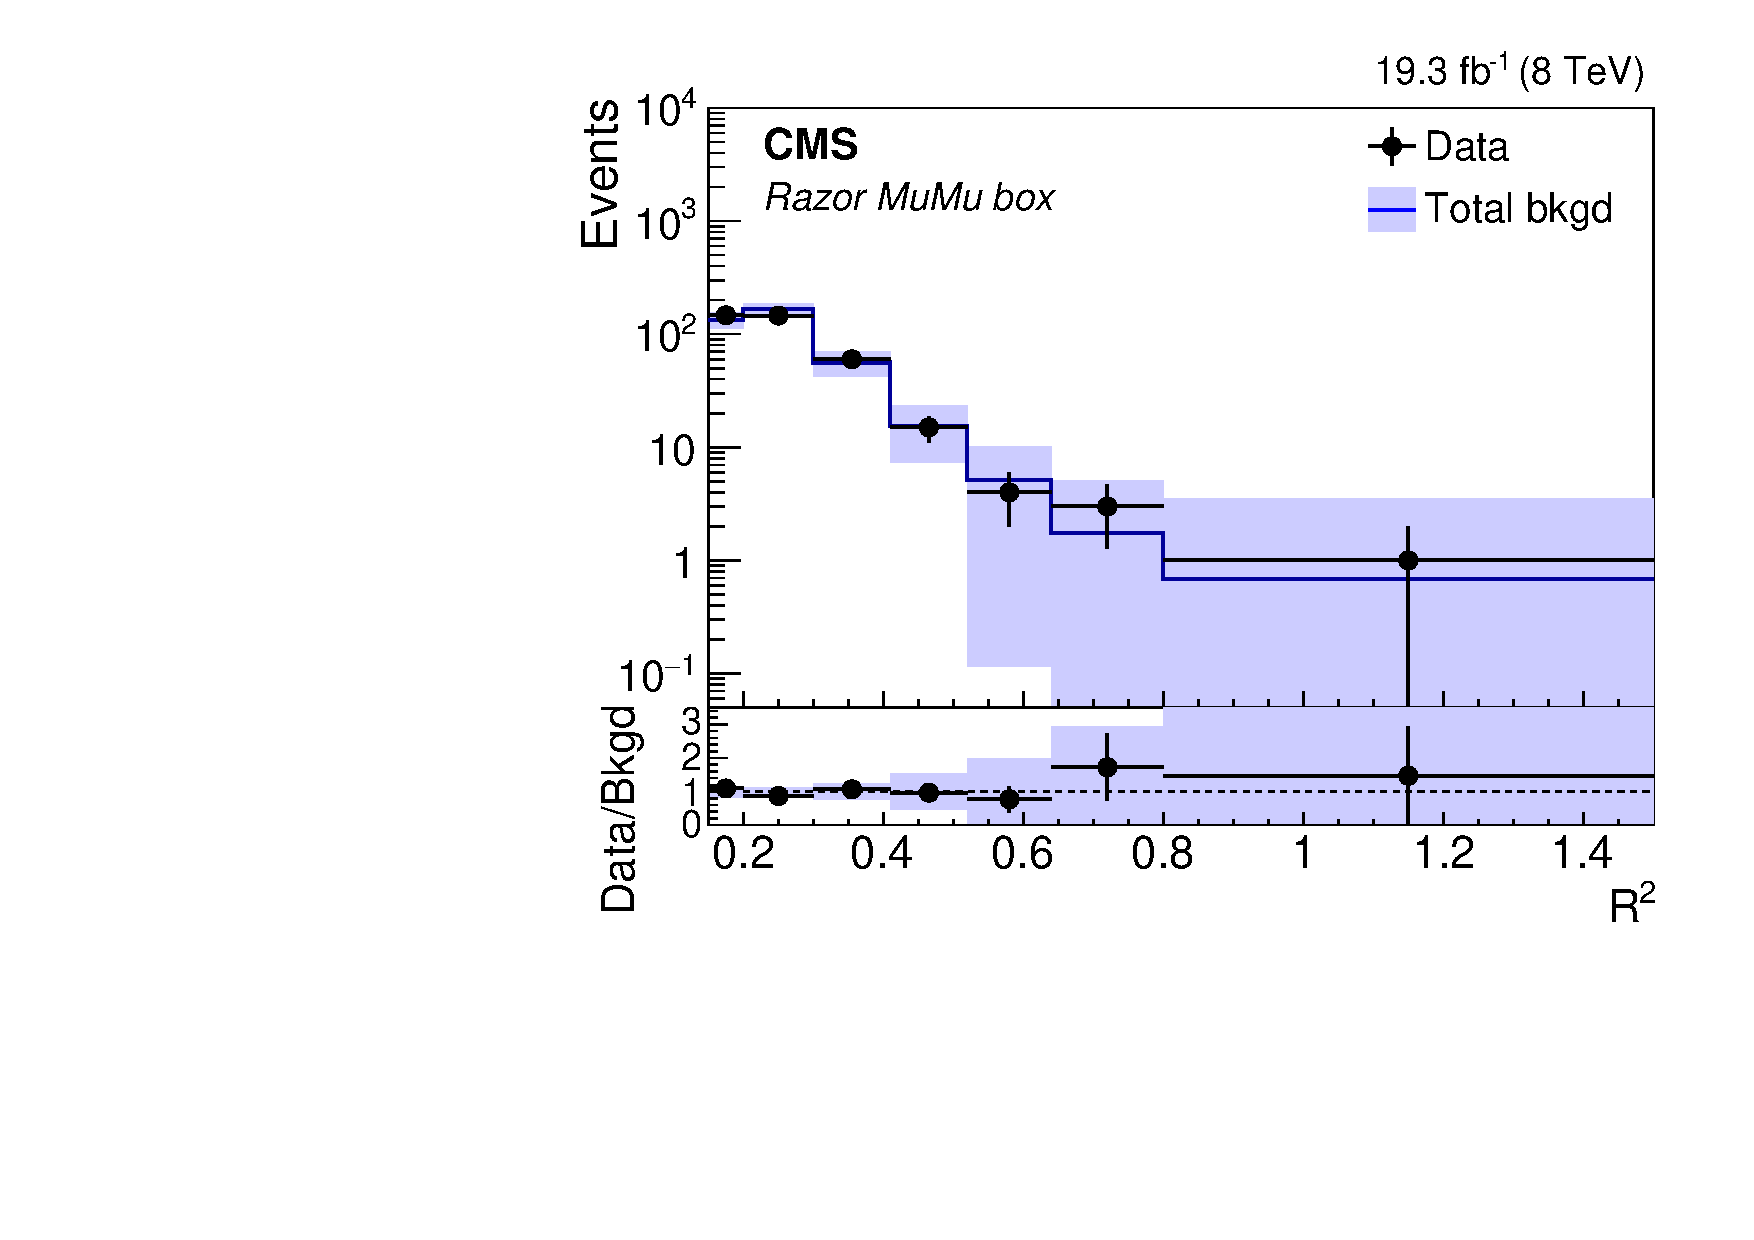
\includegraphics[width=0.49\textwidth]{figs/analysis8TeV/RSQ_MuHad-Run2012ABCD_Sideband_MuMu.pdf}
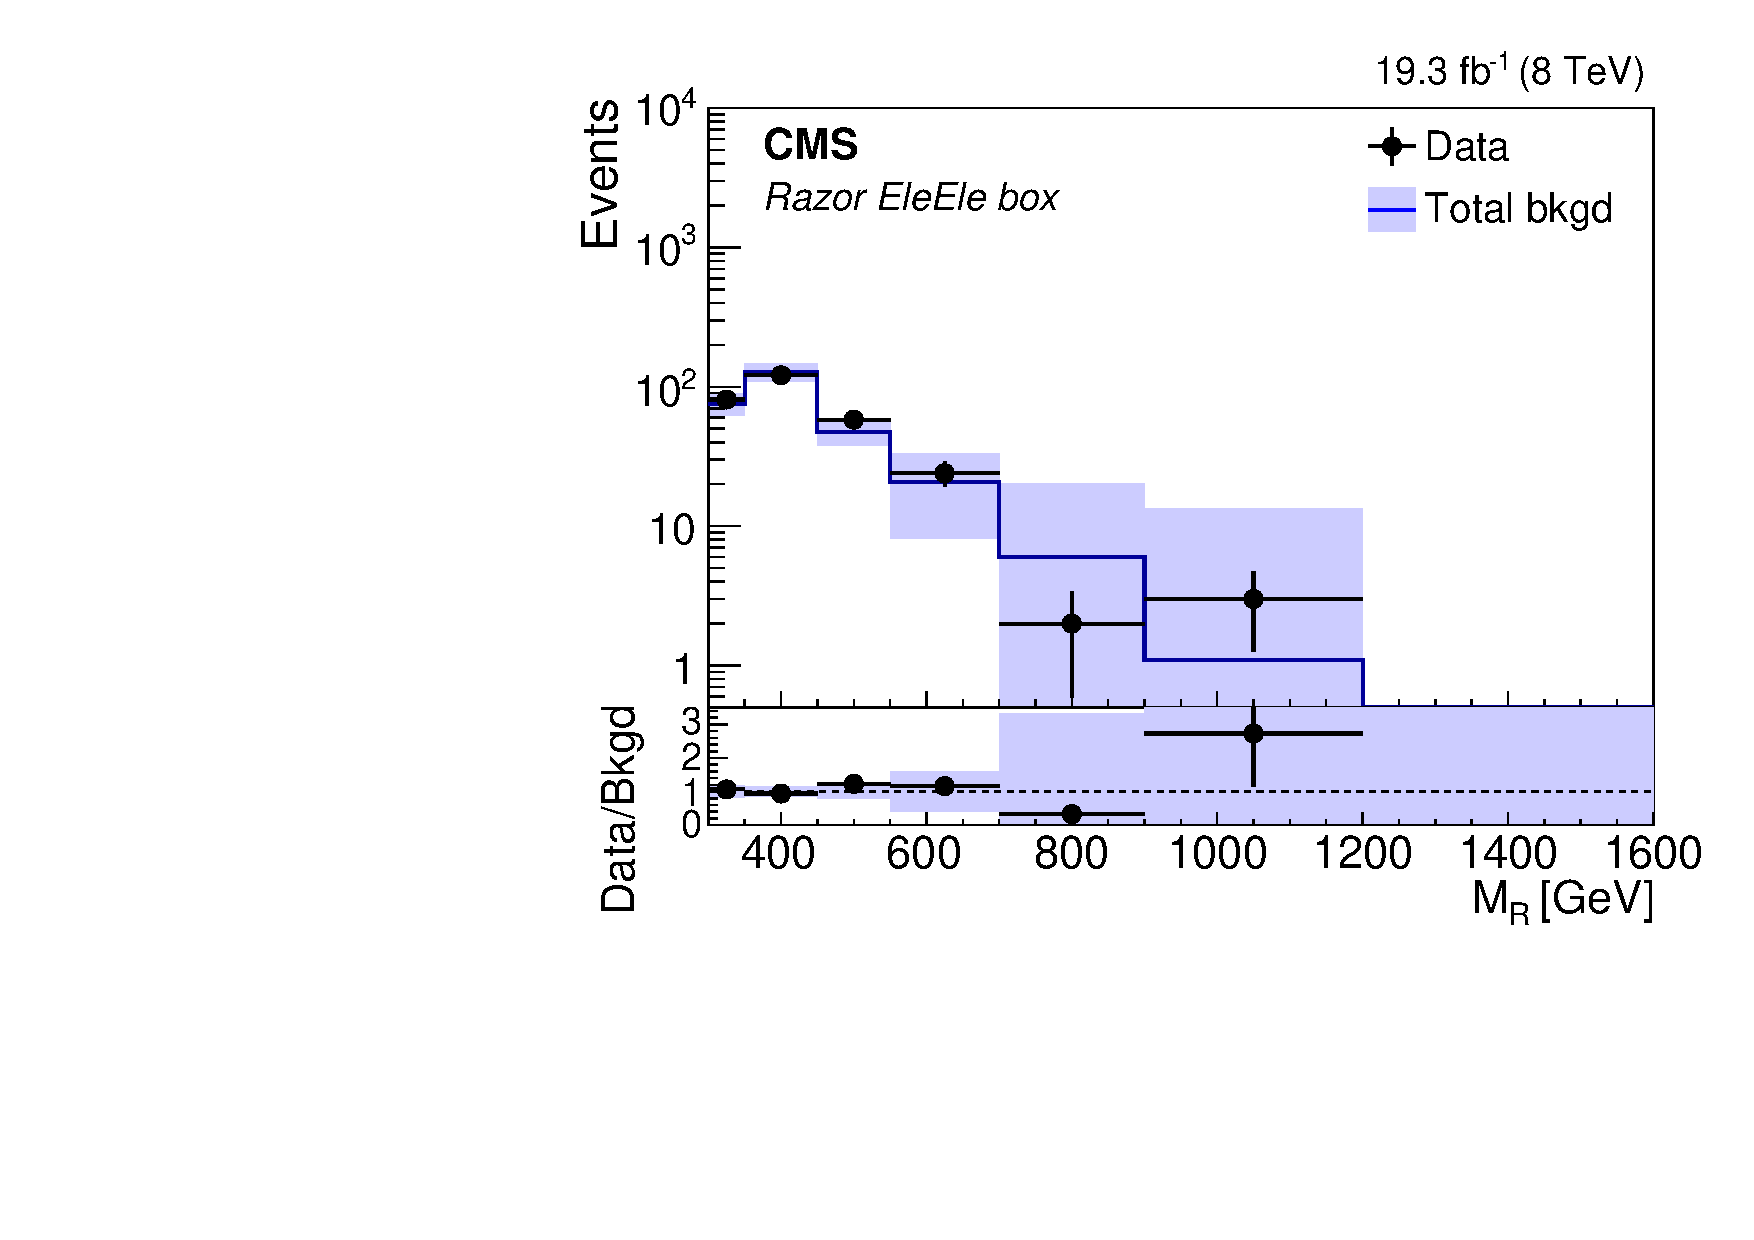
\includegraphics[width=0.49\textwidth]{figs/analysis8TeV/MR_ElectronHad-Run2012ABCD_Sideband_EleEle.pdf}
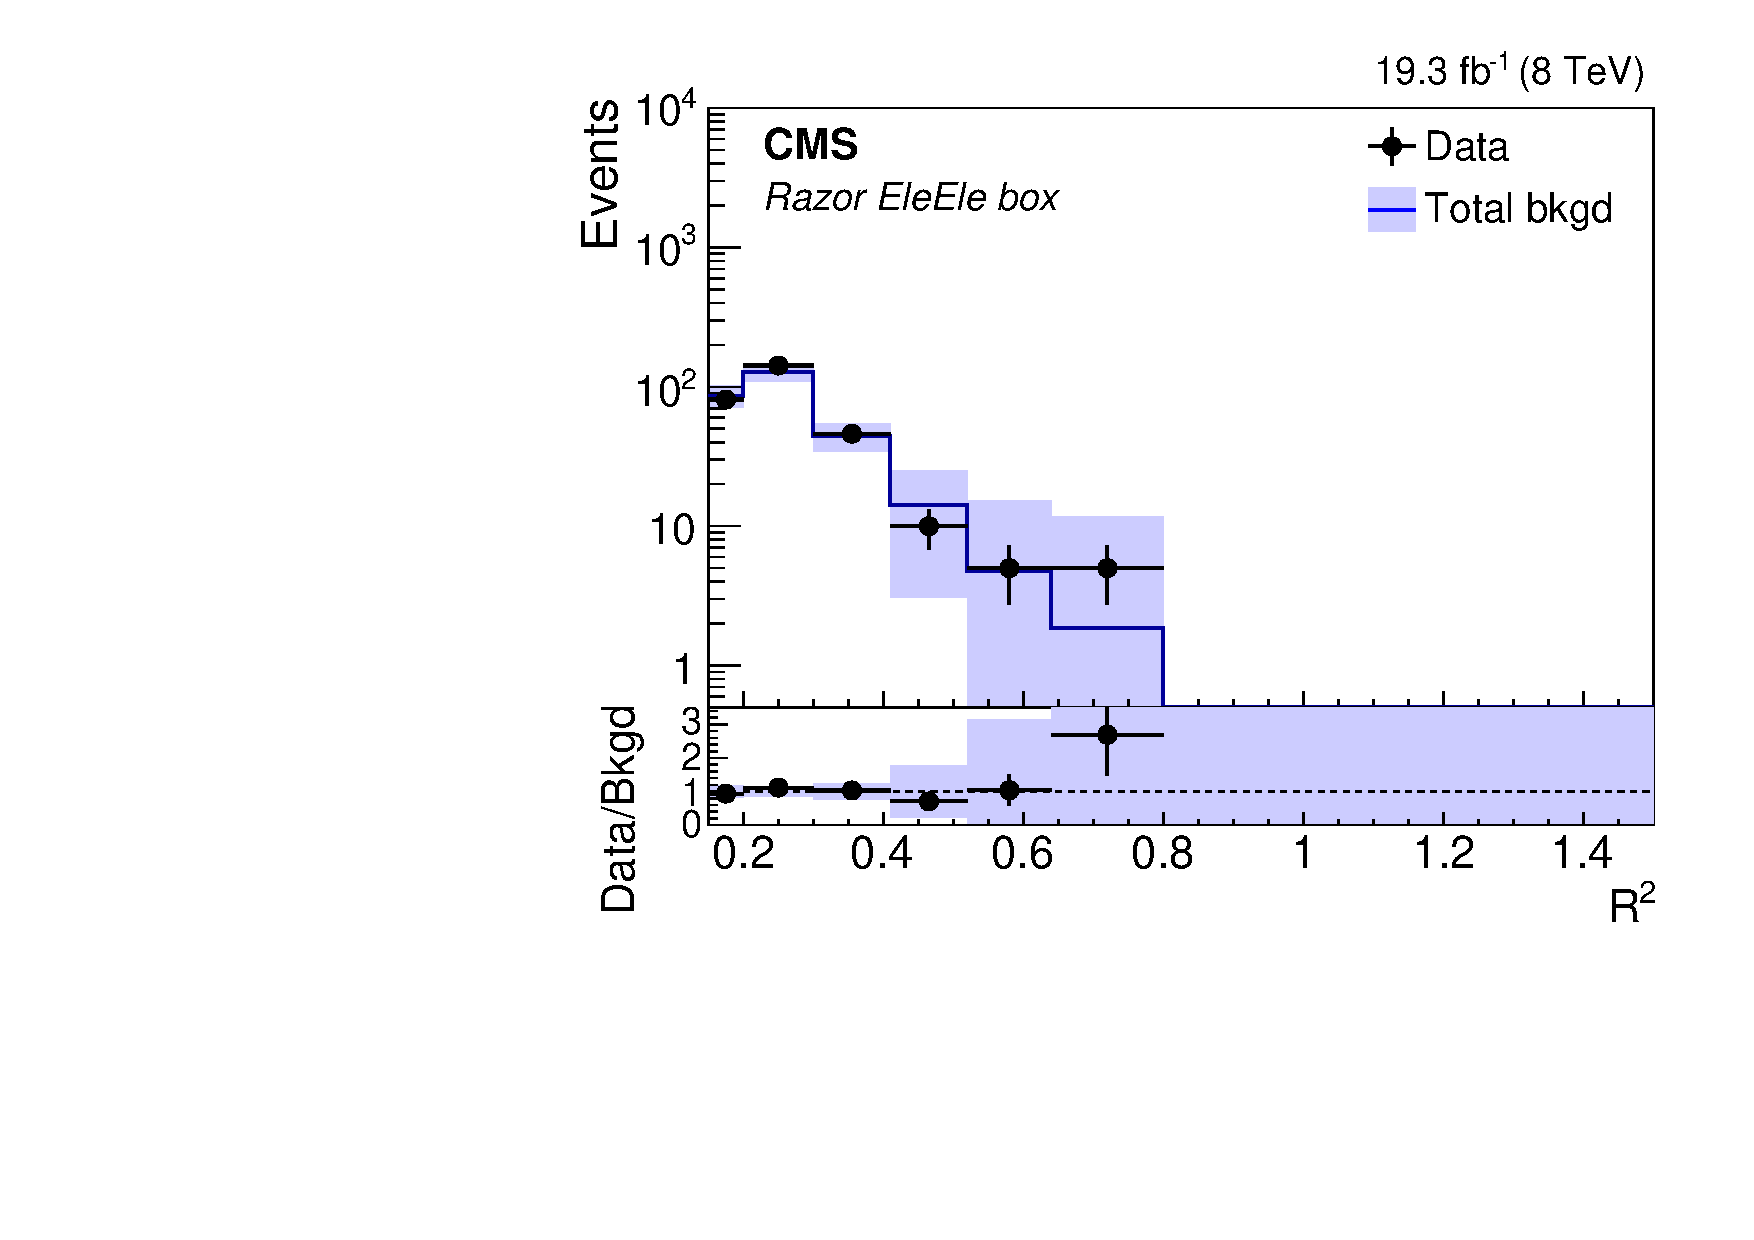
\includegraphics[width=0.49\textwidth]{figs/analysis8TeV/RSQ_ElectronHad-Run2012ABCD_Sideband_EleEle.pdf}
\caption{Projection of the sideband fit result in the (upper row) MuEle, (middle row)
  MuMu, and (lower row) EleEle boxes on \MR (left) and
   \Rtwo (right), respectively. The fit is performed
  in the sideband regions and extrapolated to the signal-sensitive
  region. The solid line and the filled band represent the total
  background prediction and its uncertainty. The points and the band
  in the bottom panel represent the data-to-prediction ratio and the
  prediction uncertainty, respectively.\label{fig:Proj1DDilep}}
\end{figure*}

\begin{figure*}[tb!]
\centering
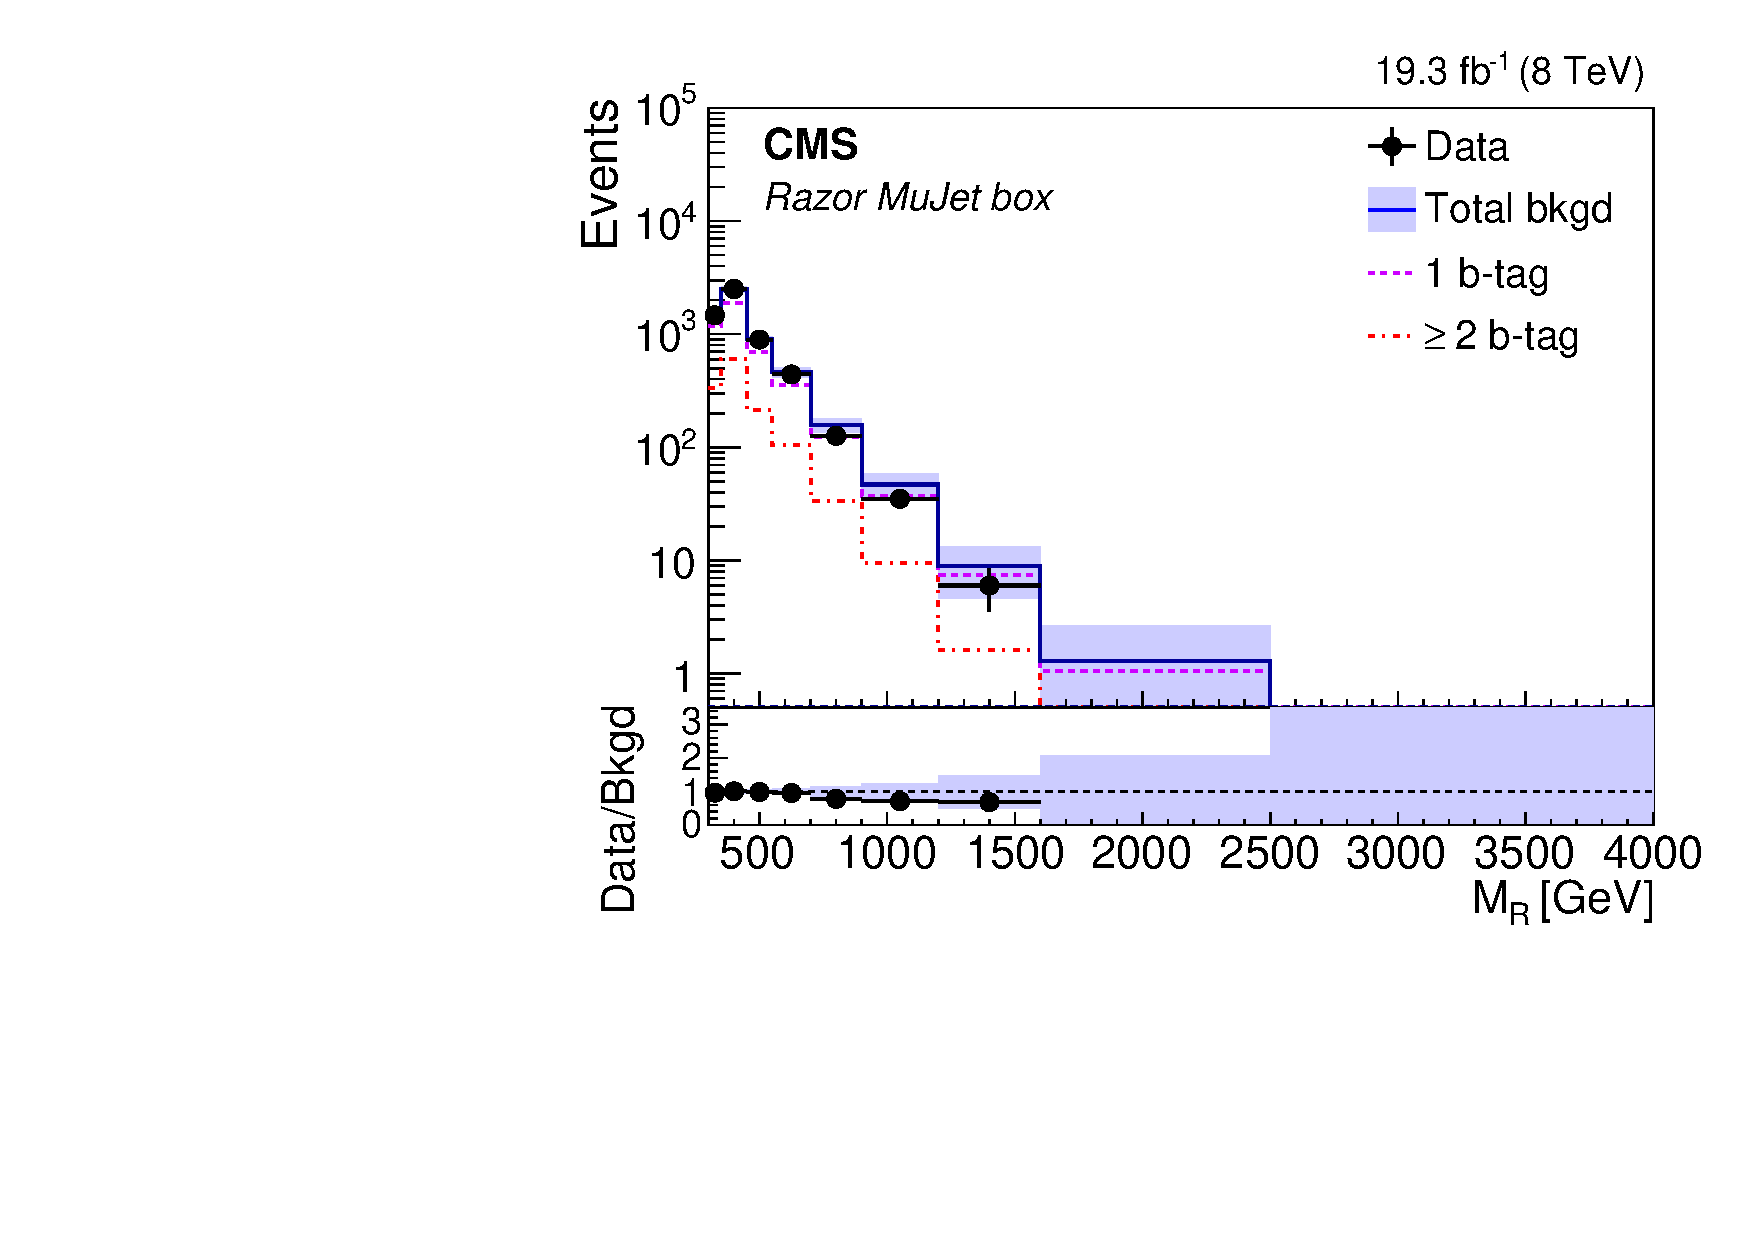
\includegraphics[width=0.49\textwidth]{figs/analysis8TeV/MR_MuHad-Run2012ABCD_Sideband_MuJet.pdf}
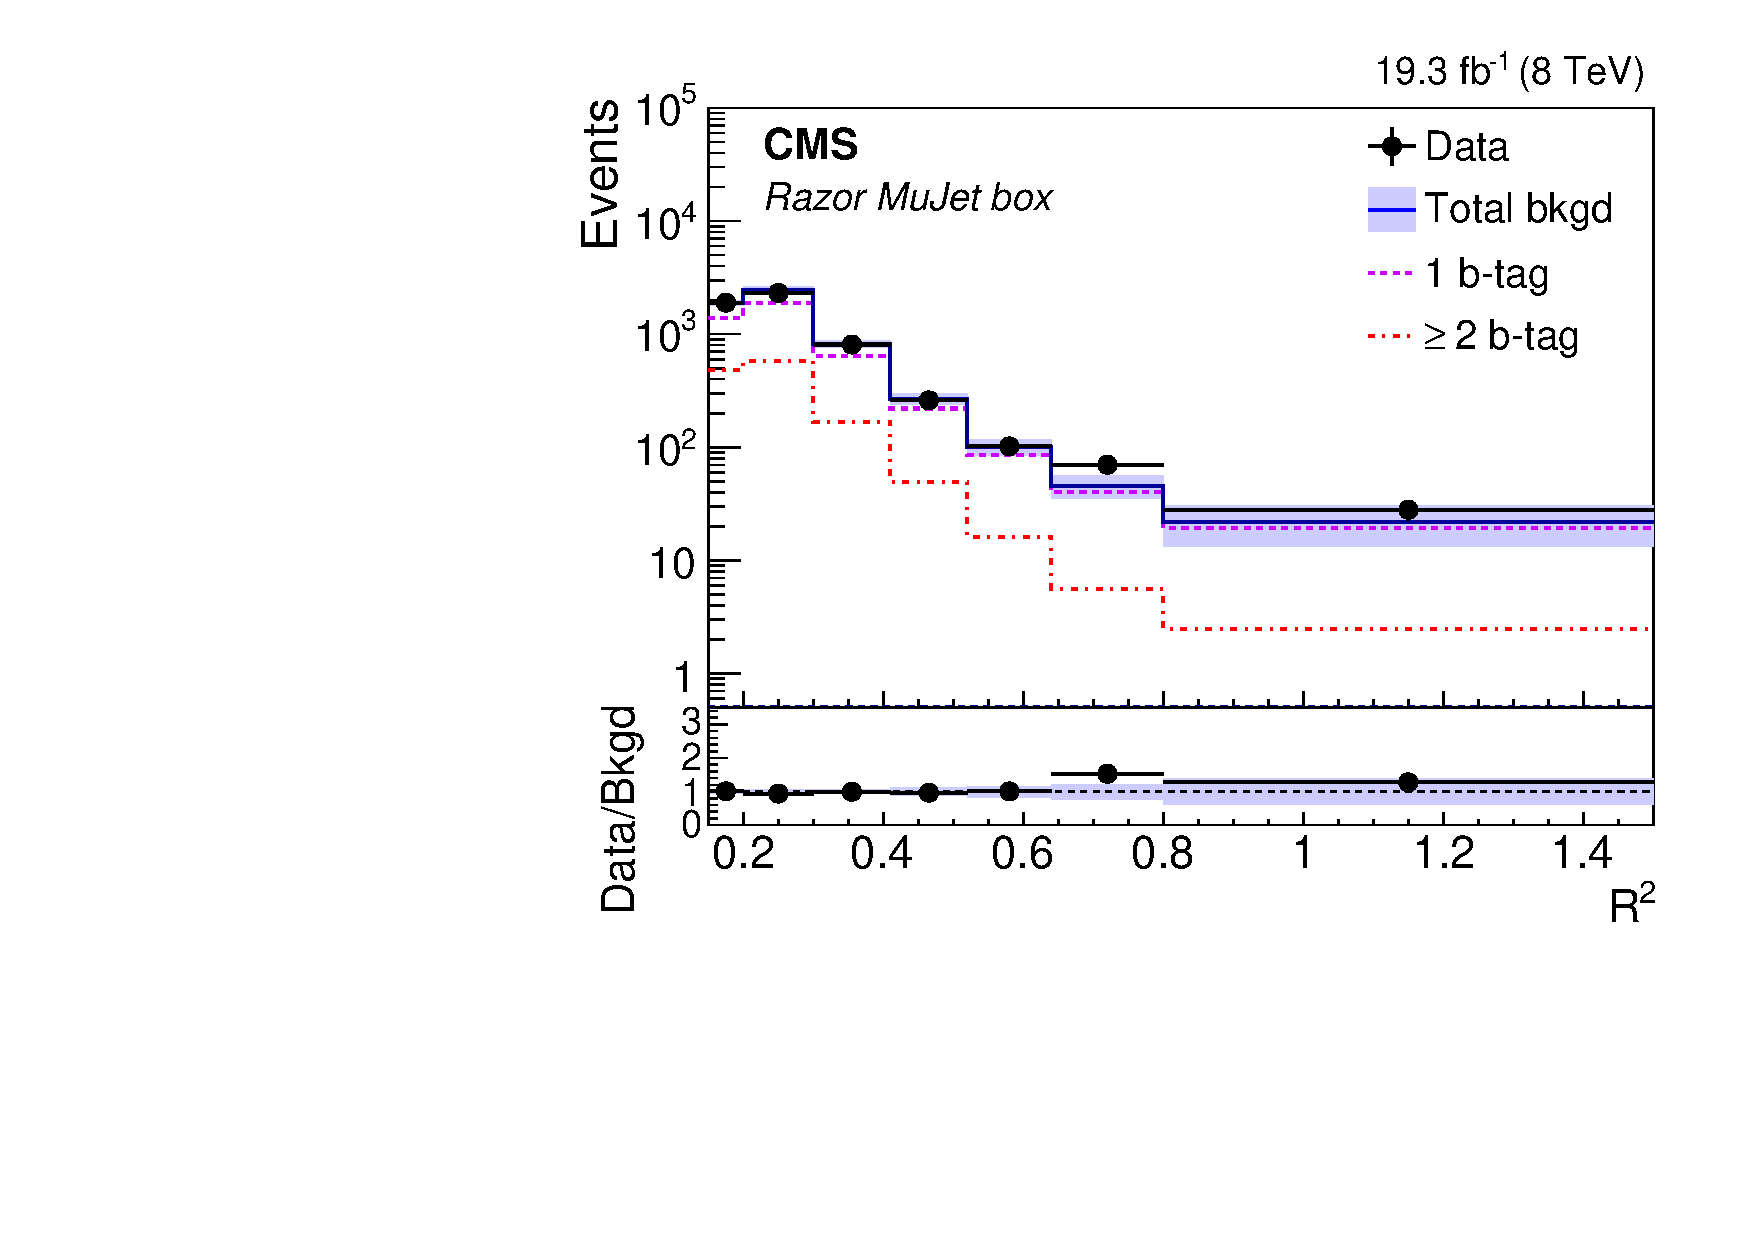
\includegraphics[width=0.49\textwidth]{figs/analysis8TeV/RSQ_MuHad-Run2012ABCD_Sideband_MuJet.pdf}
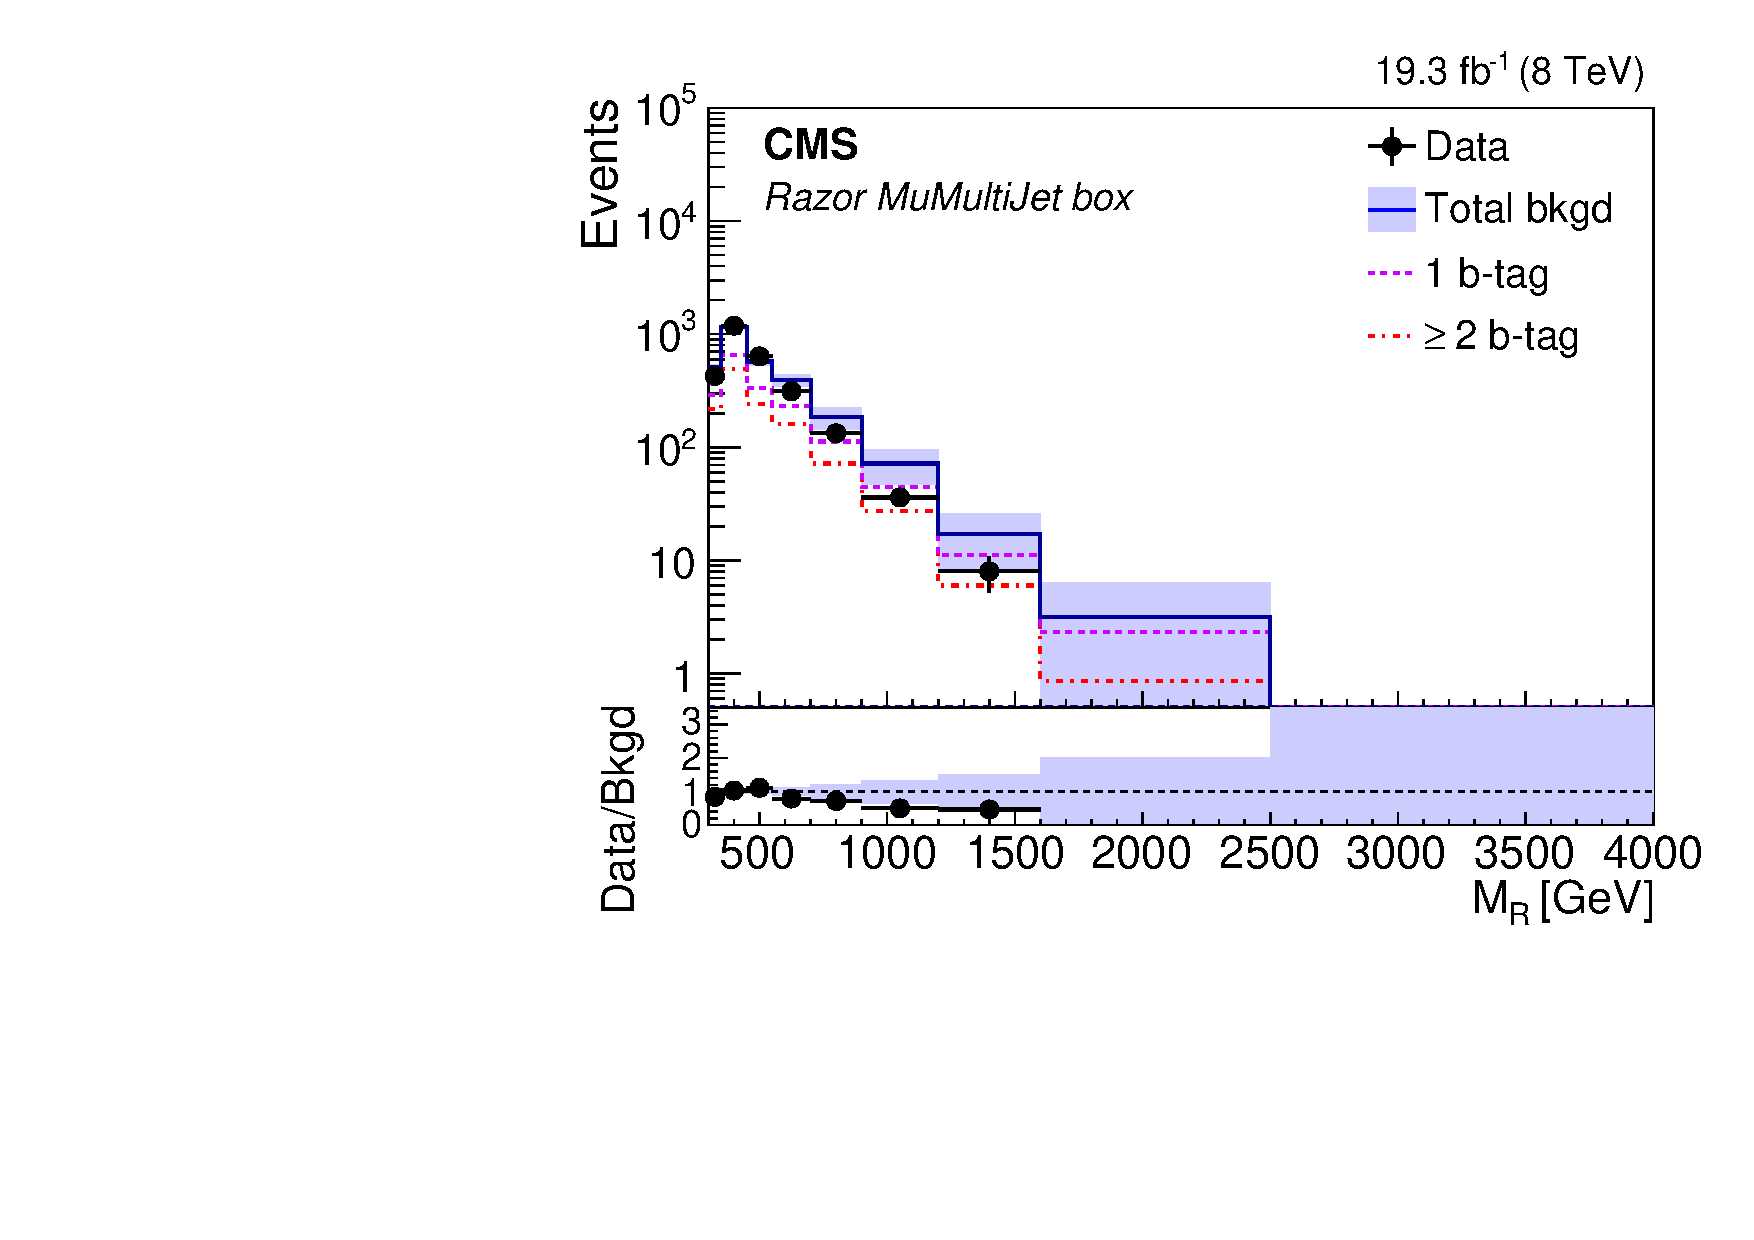
\includegraphics[width=0.49\textwidth]{figs/analysis8TeV/MR_MuHad-Run2012ABCD_Sideband_MuMultiJet.pdf}
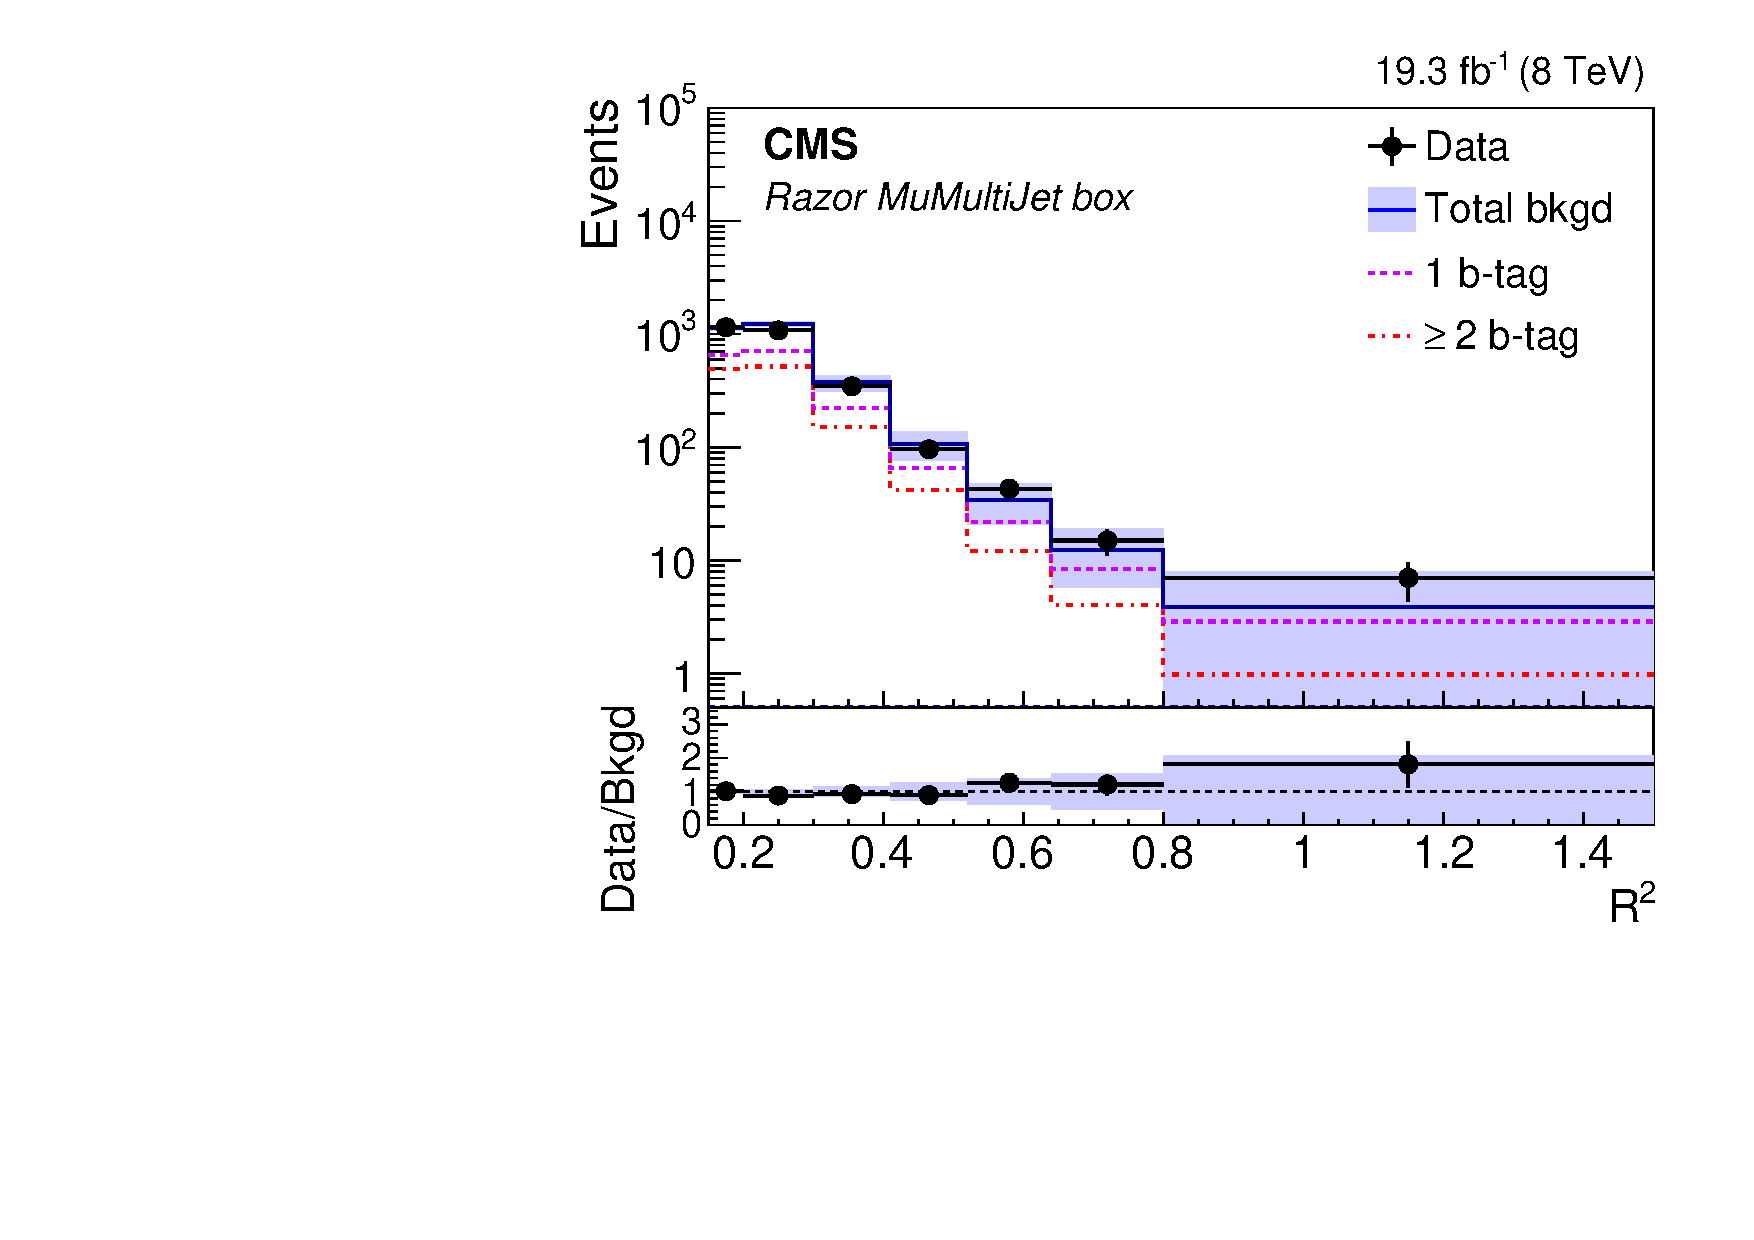
\includegraphics[width=0.49\textwidth]{figs/analysis8TeV/RSQ_MuHad-Run2012ABCD_Sideband_MuMultiJet.pdf}
\caption{Projection of the sideband fit result in the MuJet box on (upper left)
  \MR and (upper right) $\Rtwo$, and of the sideband fit
  result in the MuMultiJet box on (lower left) \MR and (lower right)
  $\Rtwo$. The fit is performed in the sideband regions and
  extrapolated to the signal-sensitive region. The solid line and the
  filled band represent the total background prediction and its
  uncertainty. The dashed and dot-dashed lines represent the
  background shape for 1 \PQb-tag and $\geq$2 \PQb-tag events,
  respectively. The points and the band in the bottom panel represent
  the data-to-prediction ratio and the prediction uncertainty,
  respectively.\label{fig:Proj1DMu}}

\end{figure*}

\begin{figure*}[tb!]
\centering
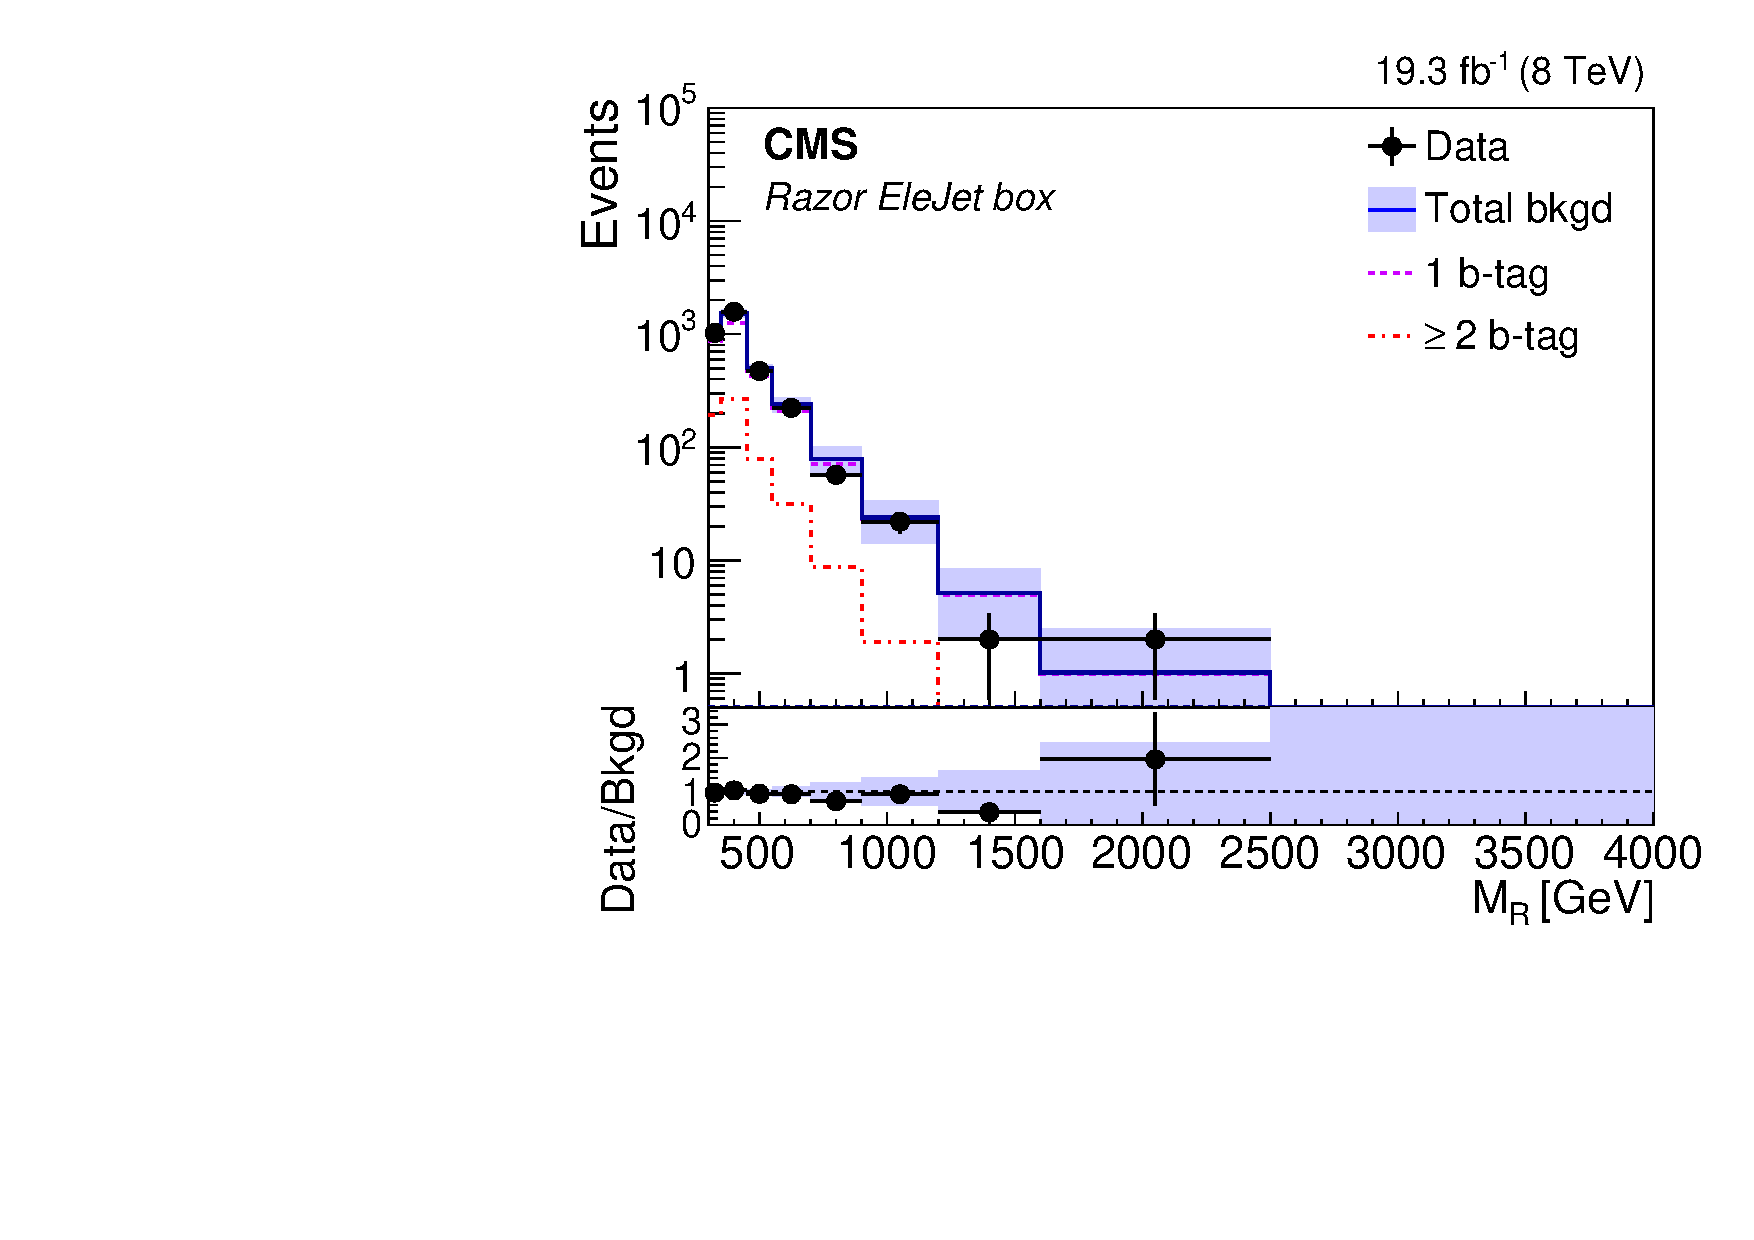
\includegraphics[width=0.49\textwidth]{figs/analysis8TeV/MR_ElectronHad-Run2012ABCD_Sideband_EleJet.pdf}
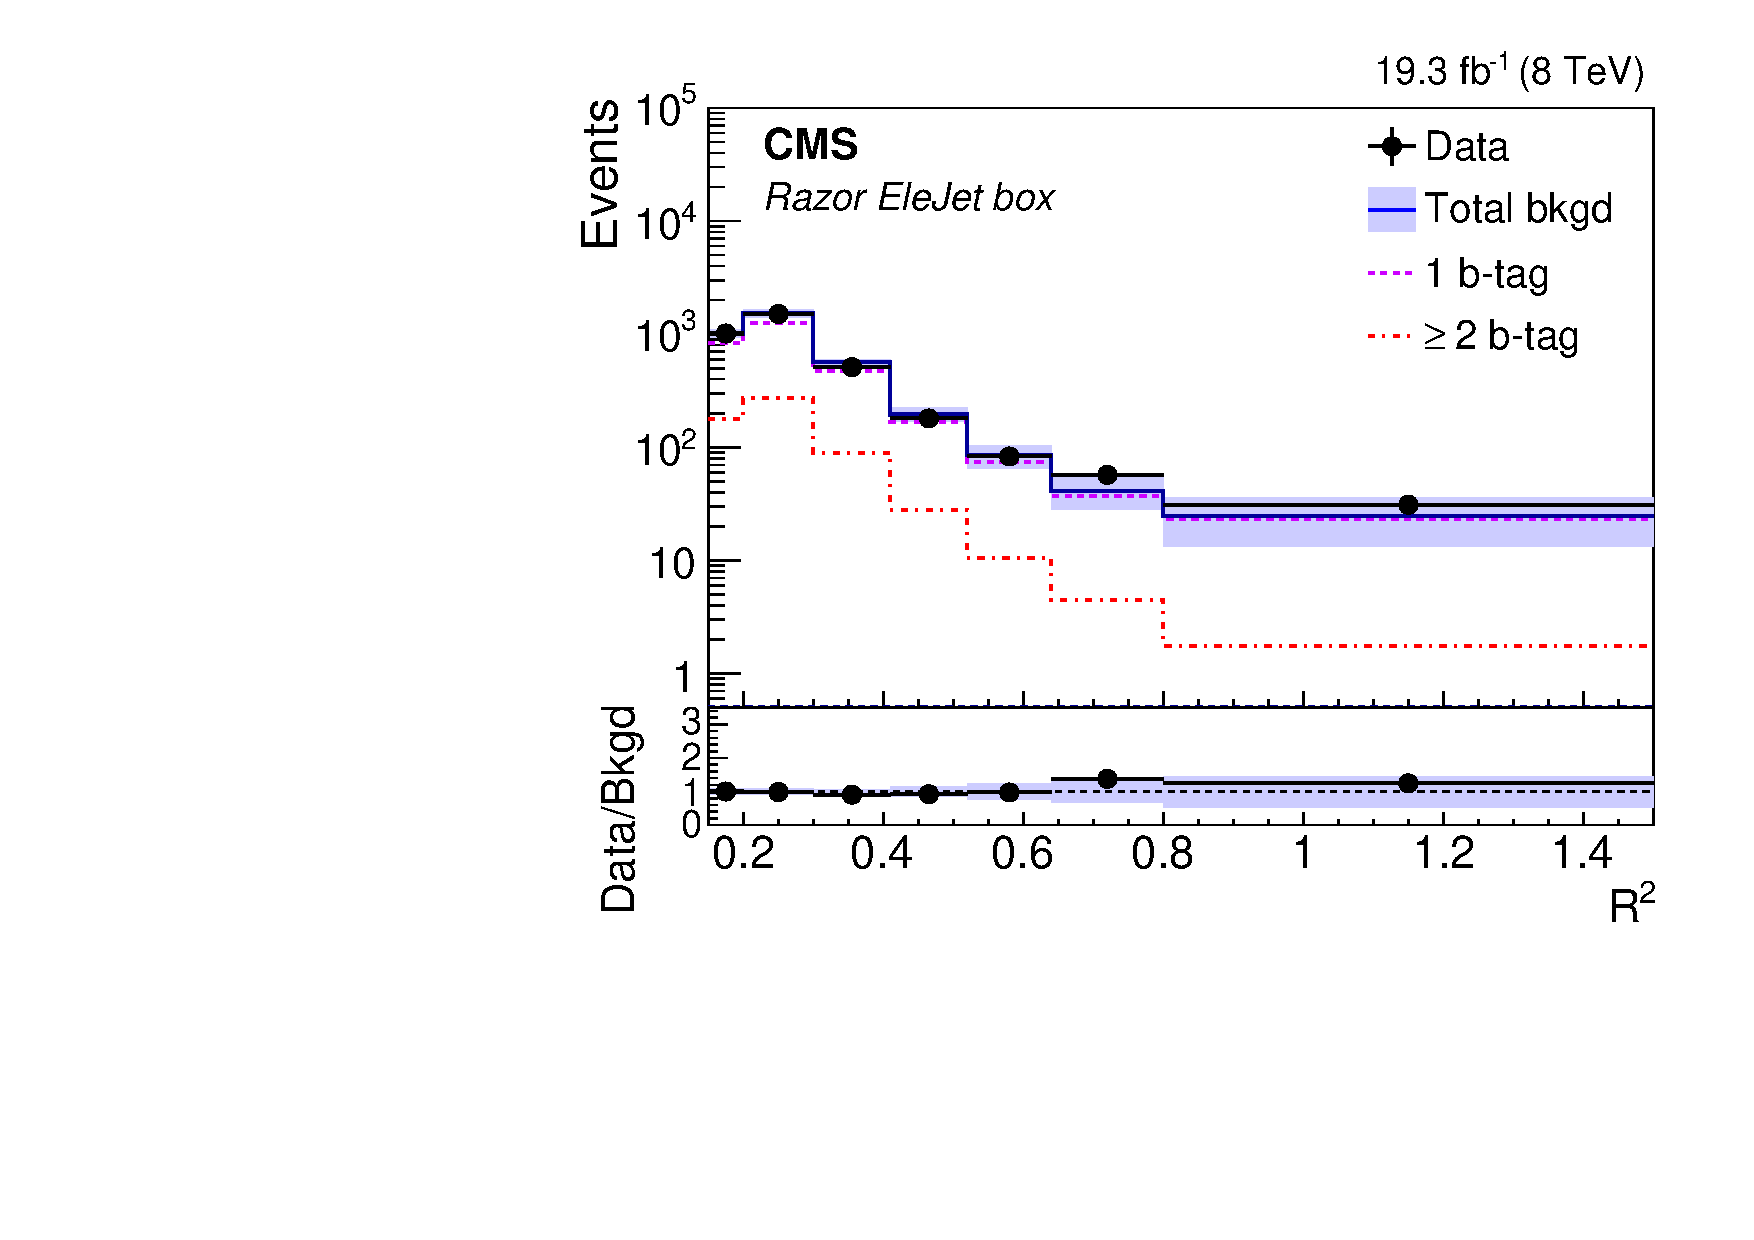
\includegraphics[width=0.49\textwidth]{figs/analysis8TeV/RSQ_ElectronHad-Run2012ABCD_Sideband_EleJet.pdf}
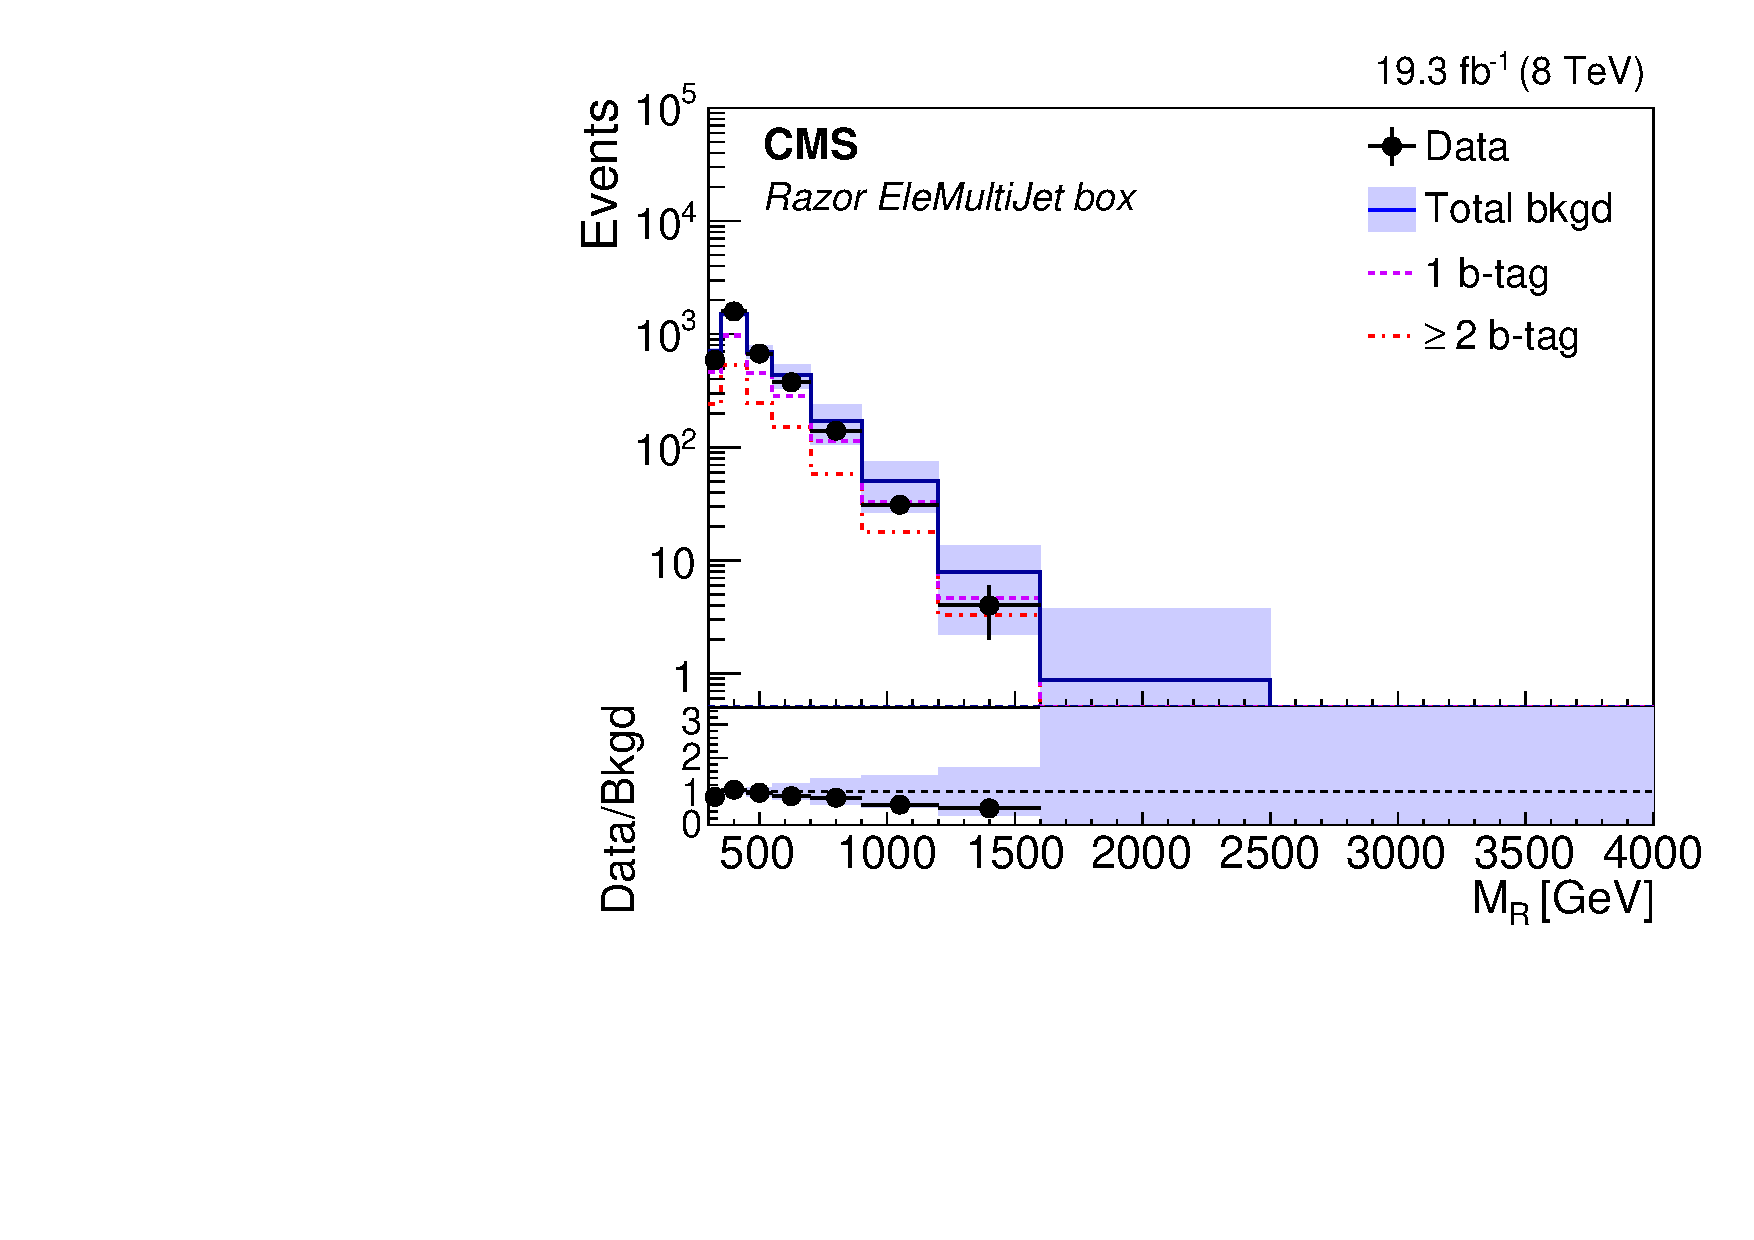
\includegraphics[width=0.49\textwidth]{figs/analysis8TeV/MR_ElectronHad-Run2012ABCD_Sideband_EleMultiJet.pdf}
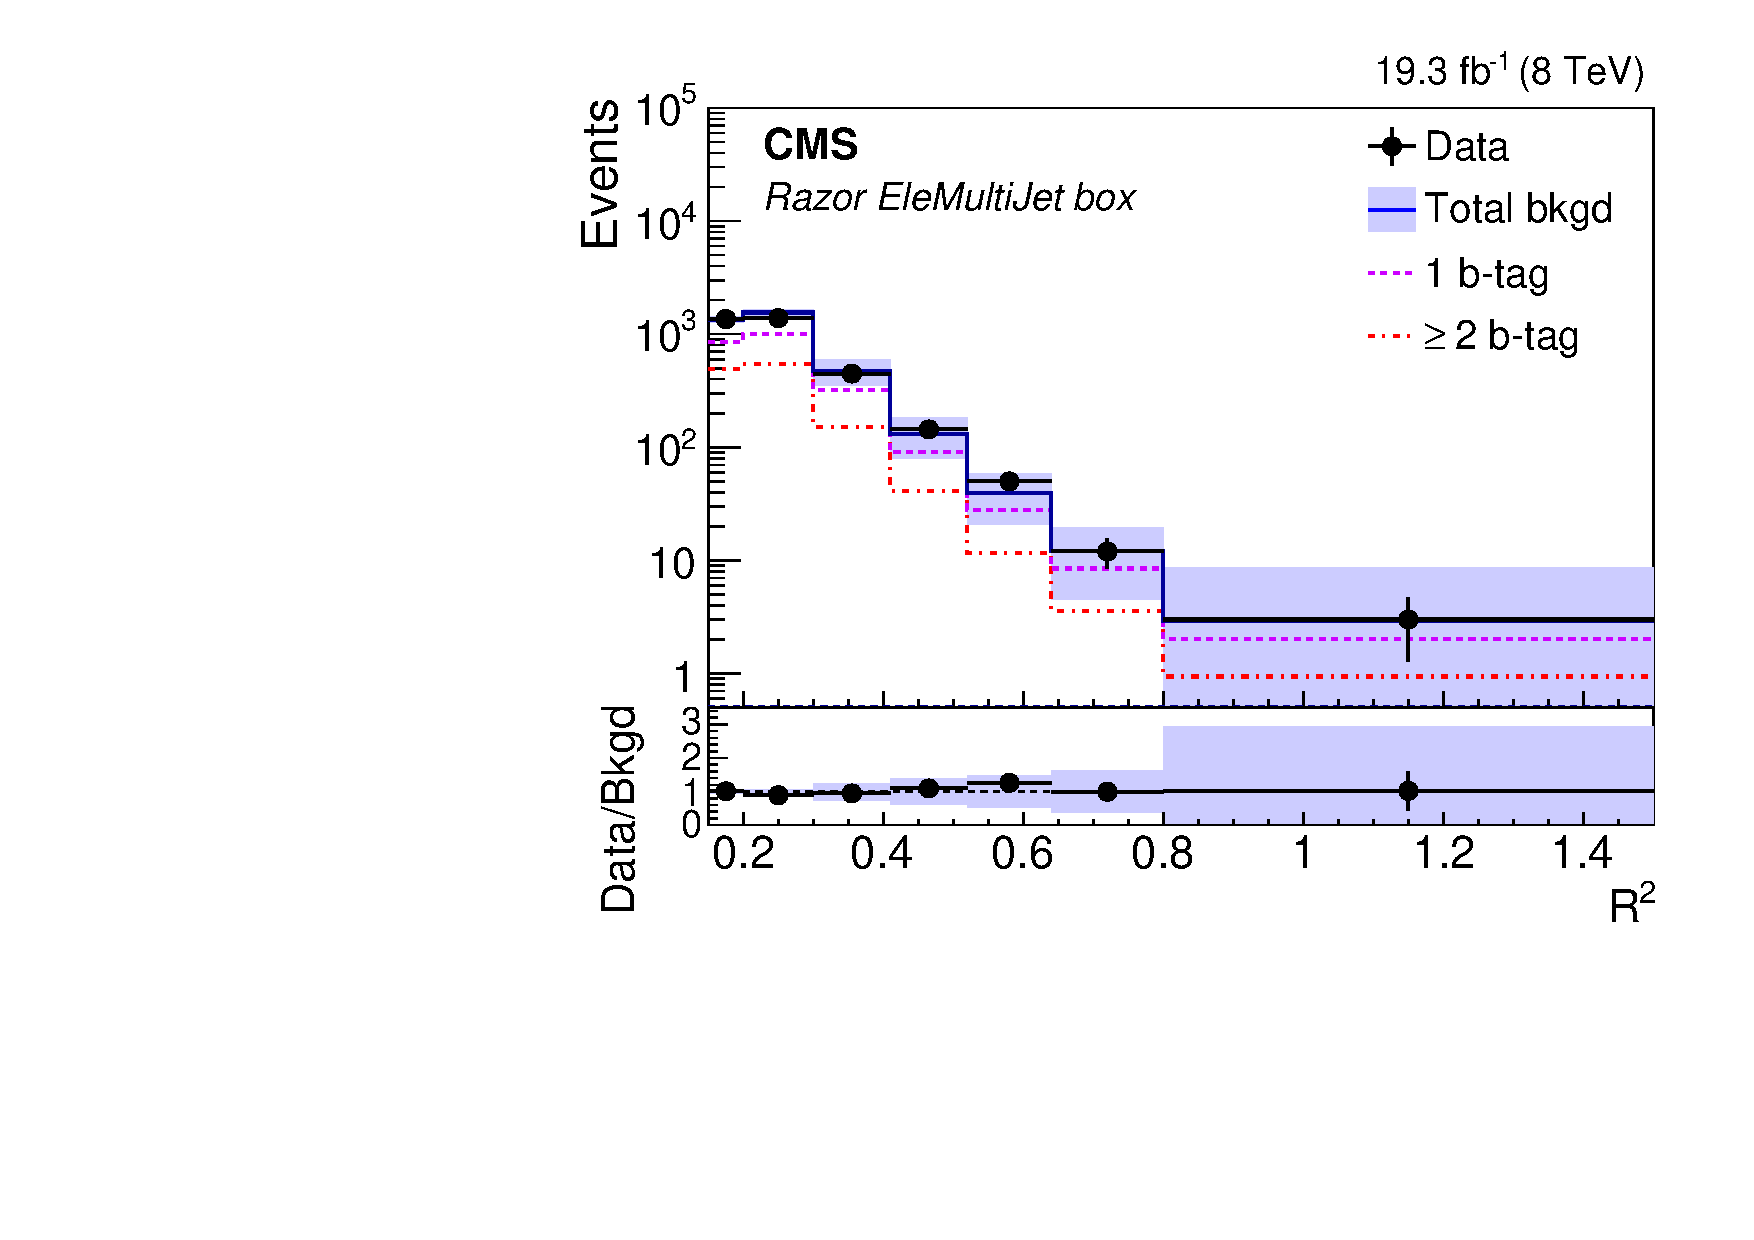
\includegraphics[width=0.49\textwidth]{figs/analysis8TeV/RSQ_ElectronHad-Run2012ABCD_Sideband_EleMultiJet.pdf}
\caption{Projection of the sideband fit result in the EleJet box on
  (upper left) \MR and (upper right) $\Rtwo$, and projection of the
  sideband fit result in the EleMultiJet box on (lower left) \MR and
  (lower right) $\Rtwo$. A detailed explanation is given in the caption
  of Fig.~\ref{fig:Proj1DMu}.\label{fig:Proj1DEle}}
\end{figure*}

\begin{figure*}[tb!]
\centering
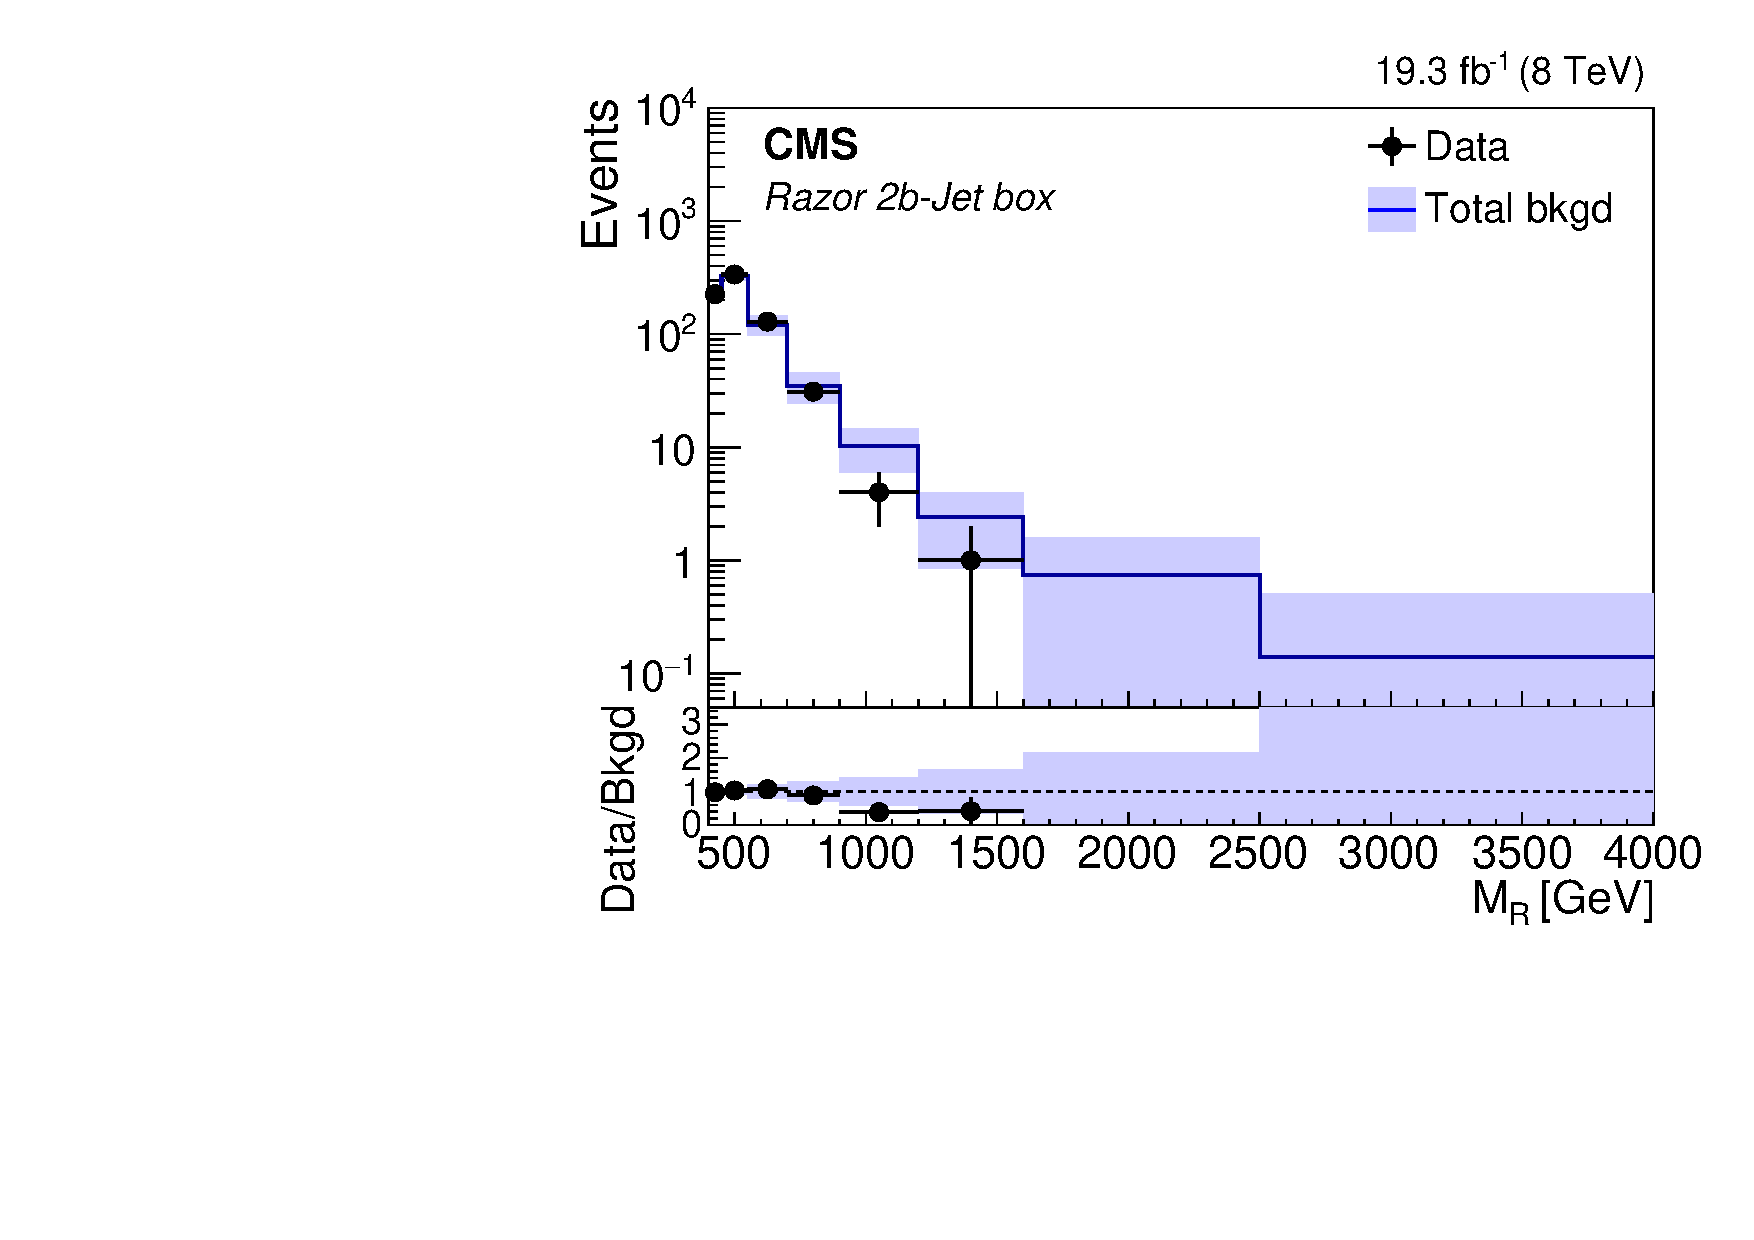
\includegraphics[width=0.49\textwidth]{figs/analysis8TeV/MR_HT-HTMHT-Run2012ABCD_Sideband_Jet2b.pdf}
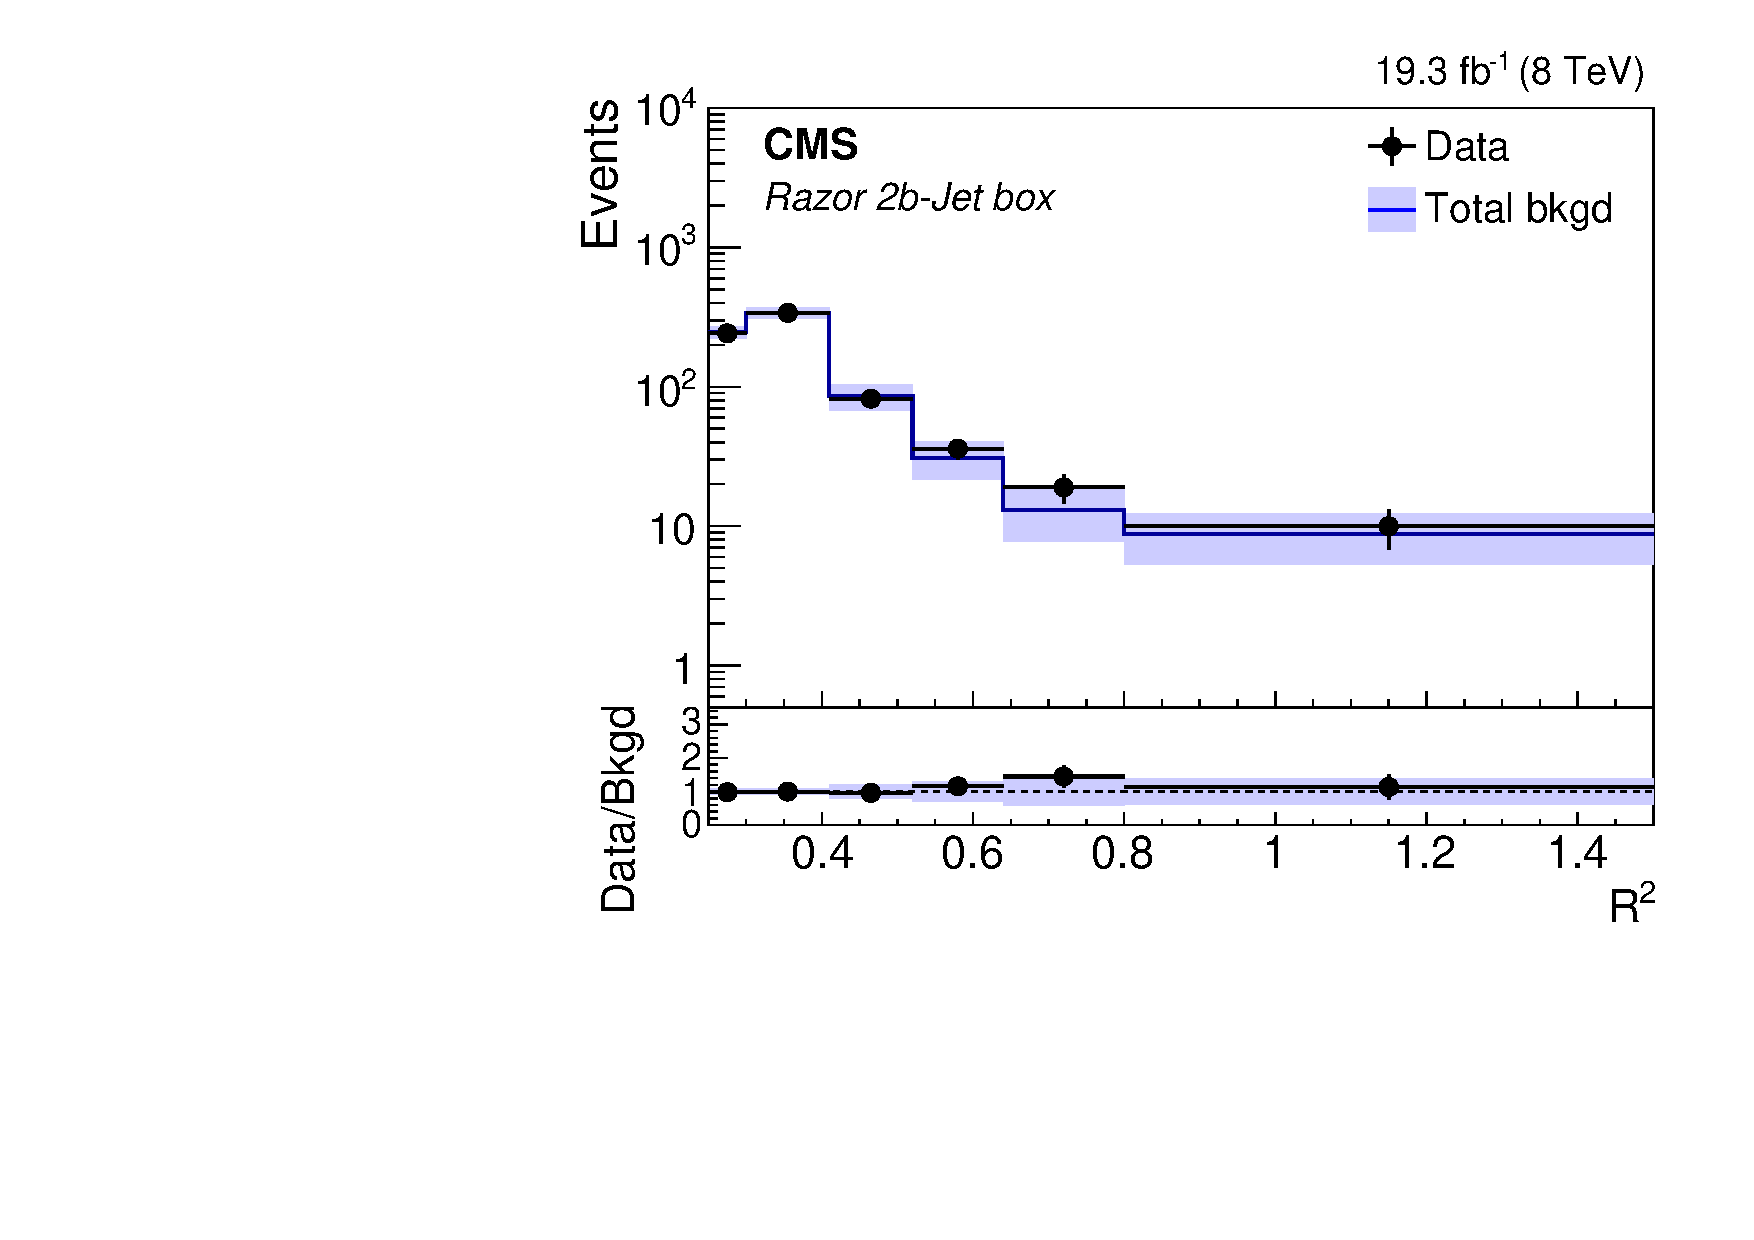
\includegraphics[width=0.49\textwidth]{figs/analysis8TeV/RSQ_HT-HTMHT-Run2012ABCD_Sideband_Jet2b.pdf}
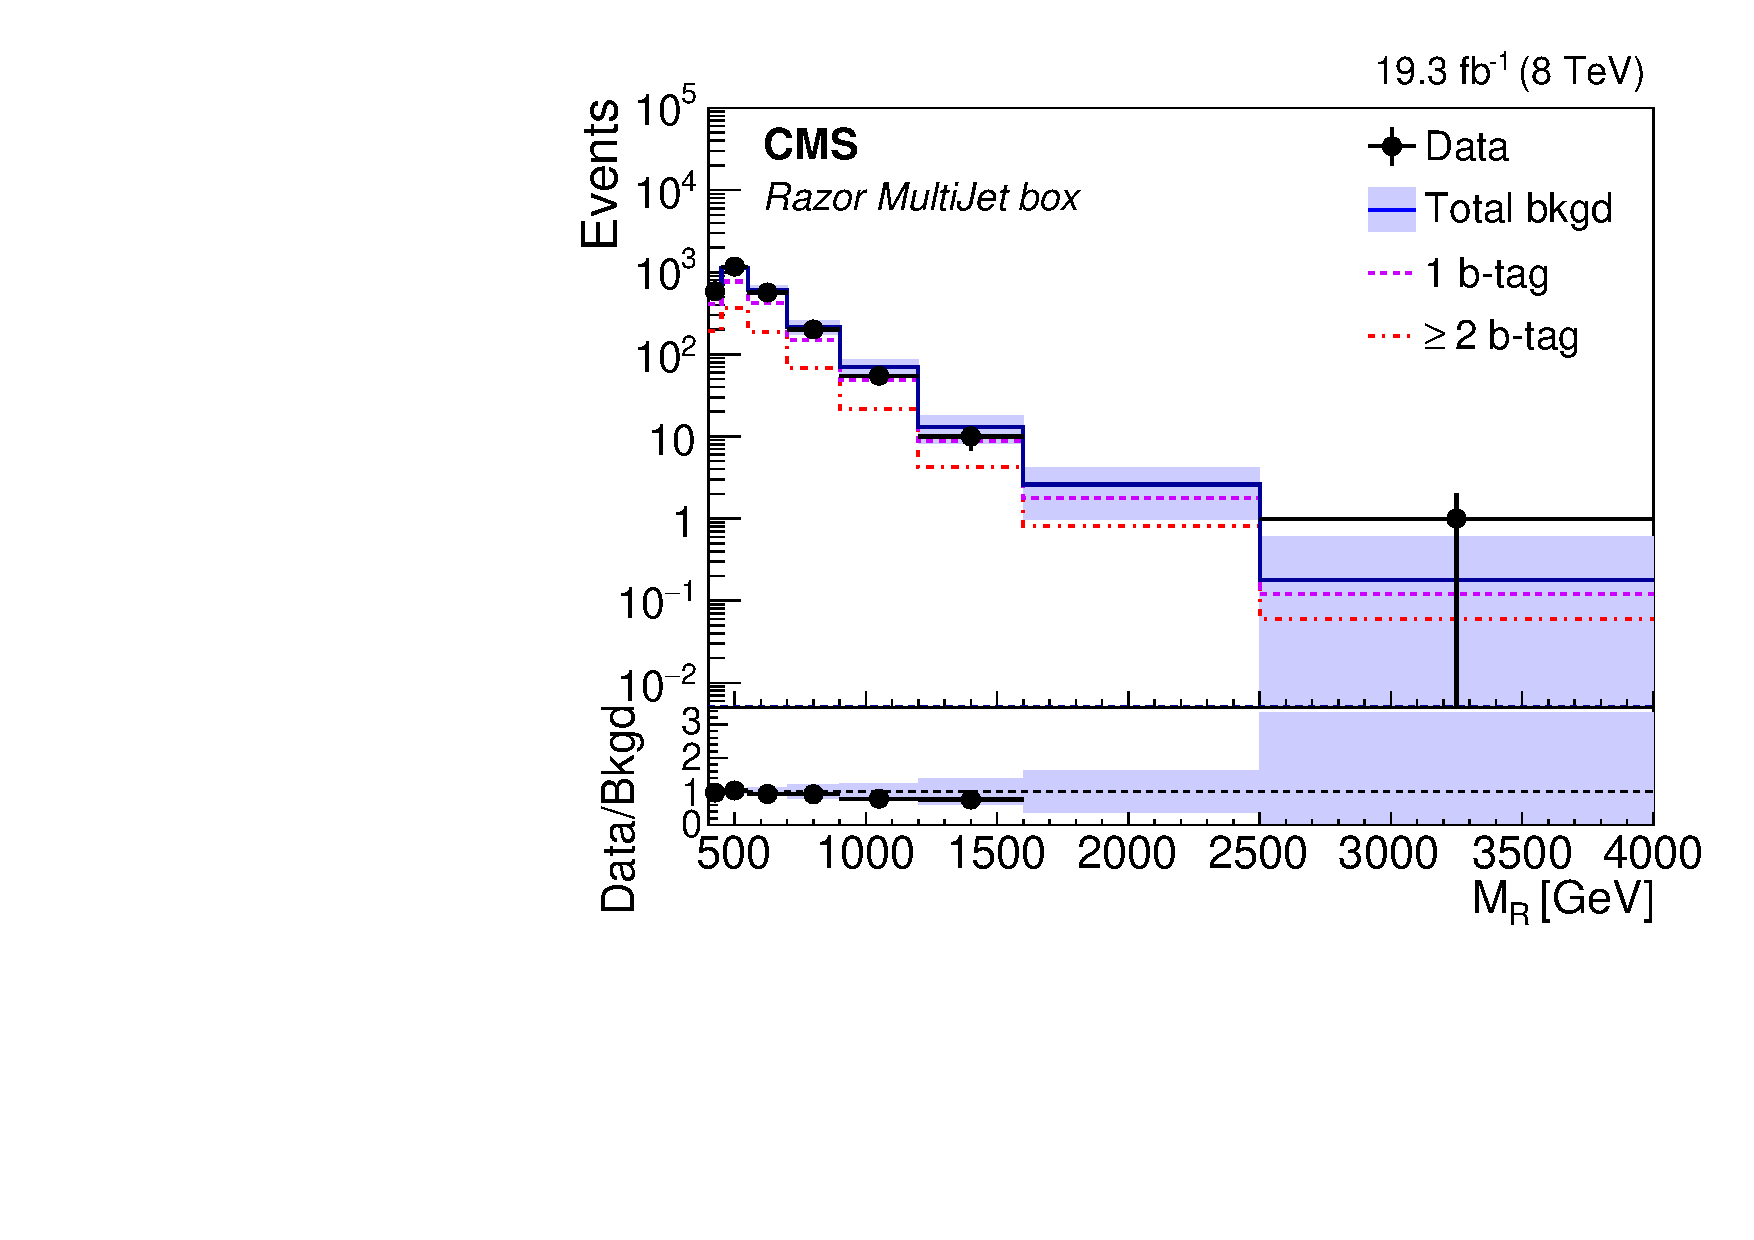
\includegraphics[width=0.49\textwidth]{figs/analysis8TeV/MR_HT-HTMHT-Run2012ABCD_Sideband_MultiJet.pdf}
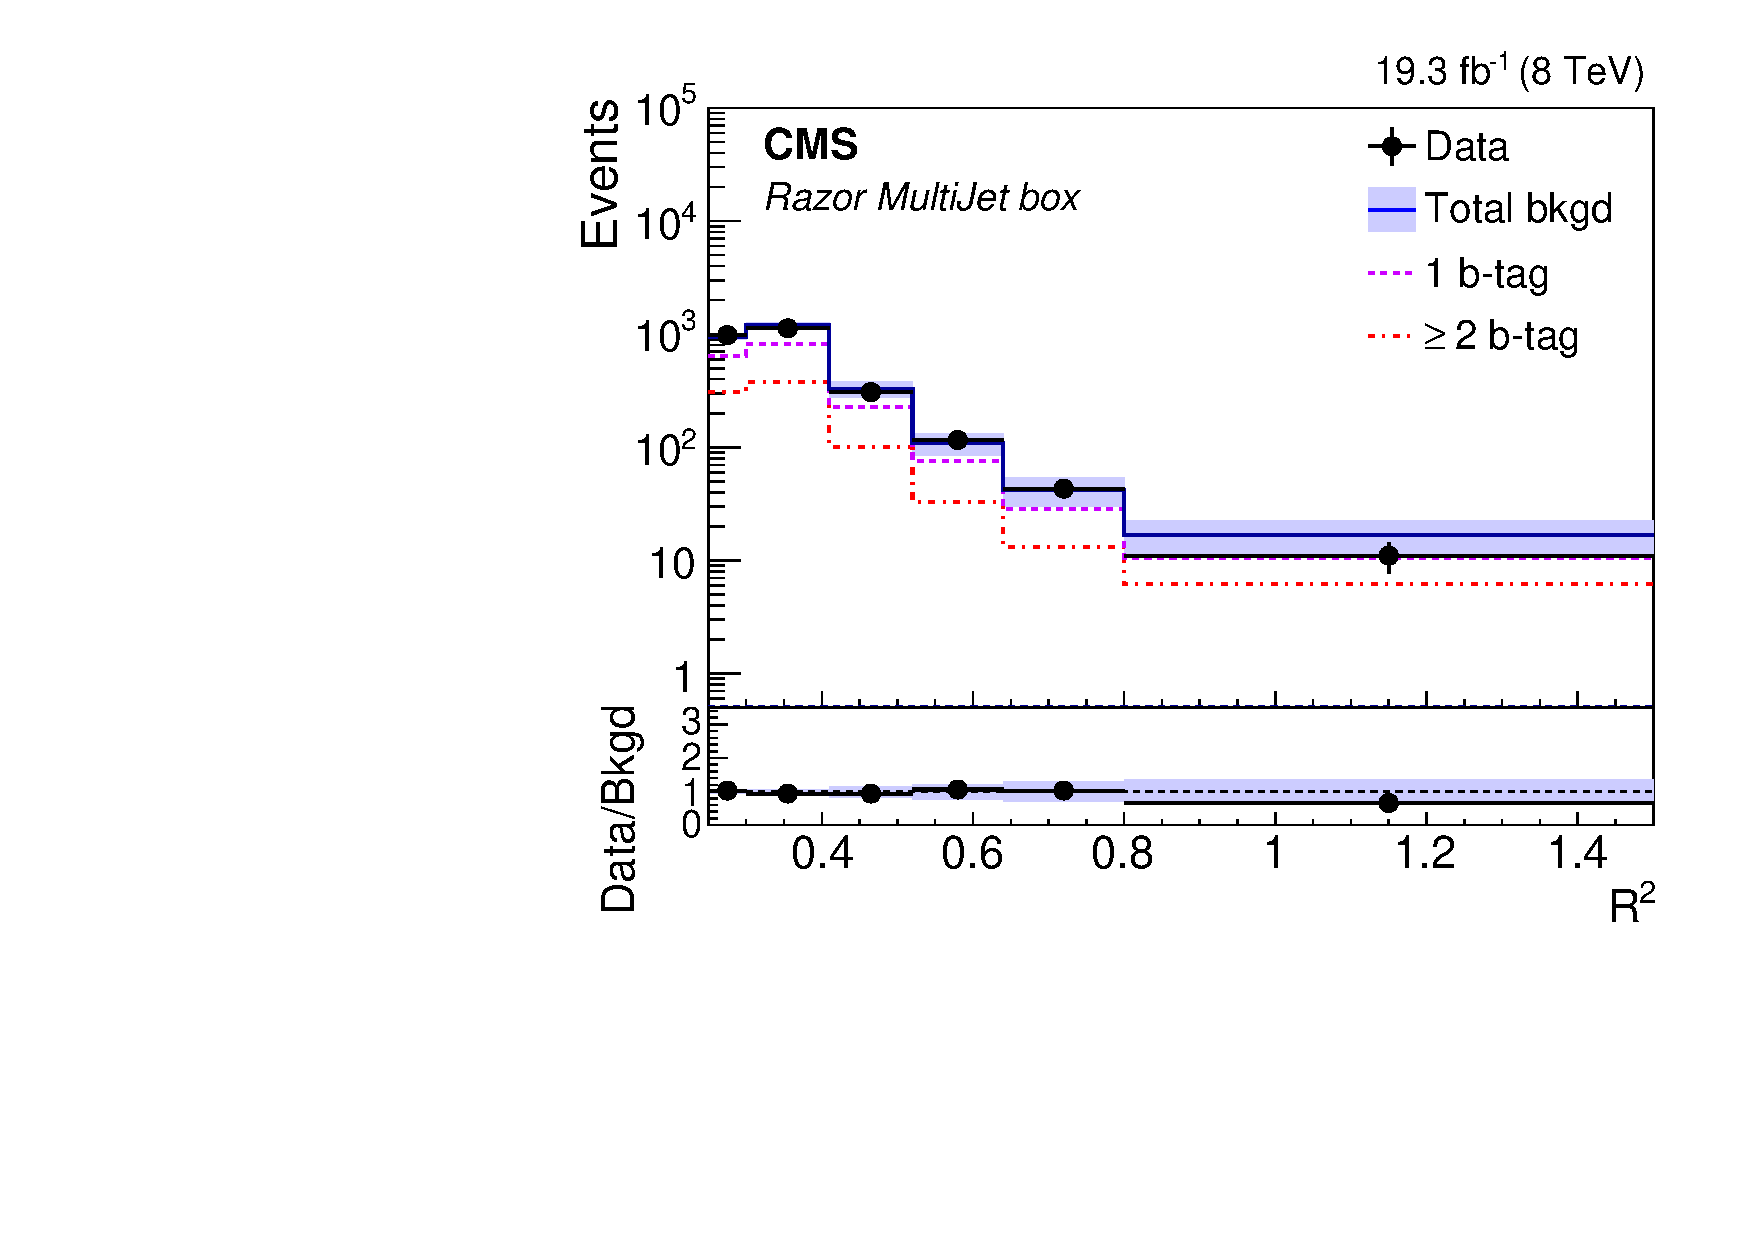
\includegraphics[width=0.49\textwidth]{figs/analysis8TeV/RSQ_HT-HTMHT-Run2012ABCD_Sideband_MultiJet.pdf}
\caption{Projection of the sideband fit result in the $\geq$2 \PQb-tagged jet
  box on (upper left) \MR and (upper right) $\Rtwo$, and projection of
  the sideband fit result in the MultiJet box on (lower left) \MR   and (lower right) $\Rtwo$. A detailed explanation is given in the
  caption of Fig.~\ref{fig:Proj1DMu}.\label{fig:Proj1DHad}}
\end{figure*}

To demonstrate the discovery potential of this analysis, we apply the
background-prediction procedure to a simulated signal-plus-background
MC sample. Figure~\ref{fig:T1bbbbsignalinj} shows the \MR and  \Rtwo distributions of SM background events and T1bbbb
events (Section~\ref{sec:sms}). The gluino and LSP masses are set
respectively to 1325\GeV and 50\GeV, representing a new-physics
scenario near the expected sensitivity of the analysis. A
signal-plus-background sample is obtained by adding the two
distributions of Fig.~\ref{fig:T1bbbbsignalinj}, assuming an
integrated luminosity of 19.3\fbinv and a gluino-gluino production
cross section of 0.02\unit{pb}, corresponding to 78 expected signal events
in the signal-sensitive region. The agreement between the background
prediction from the sideband fit and the yield of the
signal-plus-background pseudo-experiments is displayed in
Fig.~\ref{fig:FFsigma0p02}. The contribution of signal events to the
sideband region has a negligible impact on the determination of the
background shape, while a disagreement is observed in the
signal-sensitive region, characterized as an excess of events
clustered around $\MR\approx1300$\GeV. The excess indicates
the presence of a signal, and the position of the excess in the
$\MR$ variable provides information about the underlying SUSY
mass spectrum.

\begin{figure}[htb!]
\centering
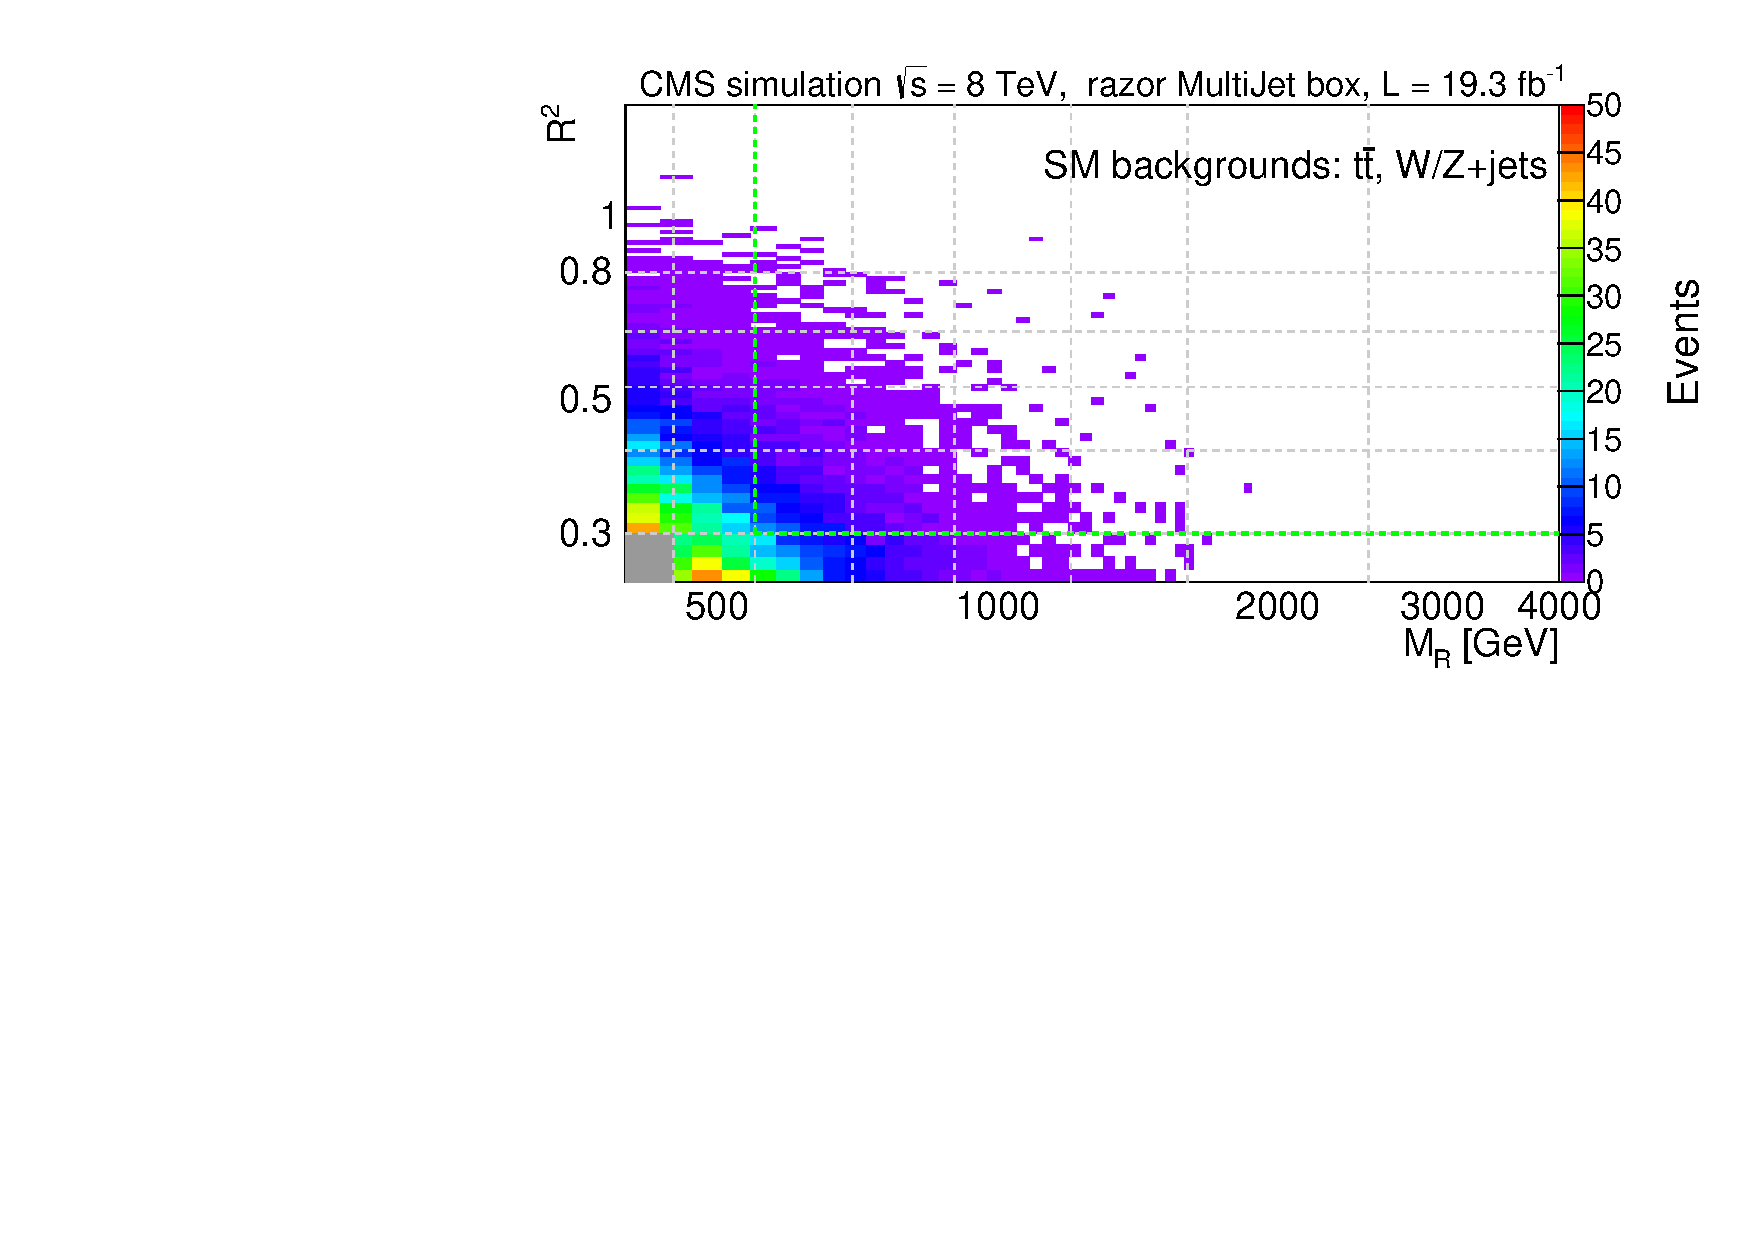
\includegraphics[width=0.49\textwidth]{figs/analysis8TeV/SMbkgd_FF.pdf}
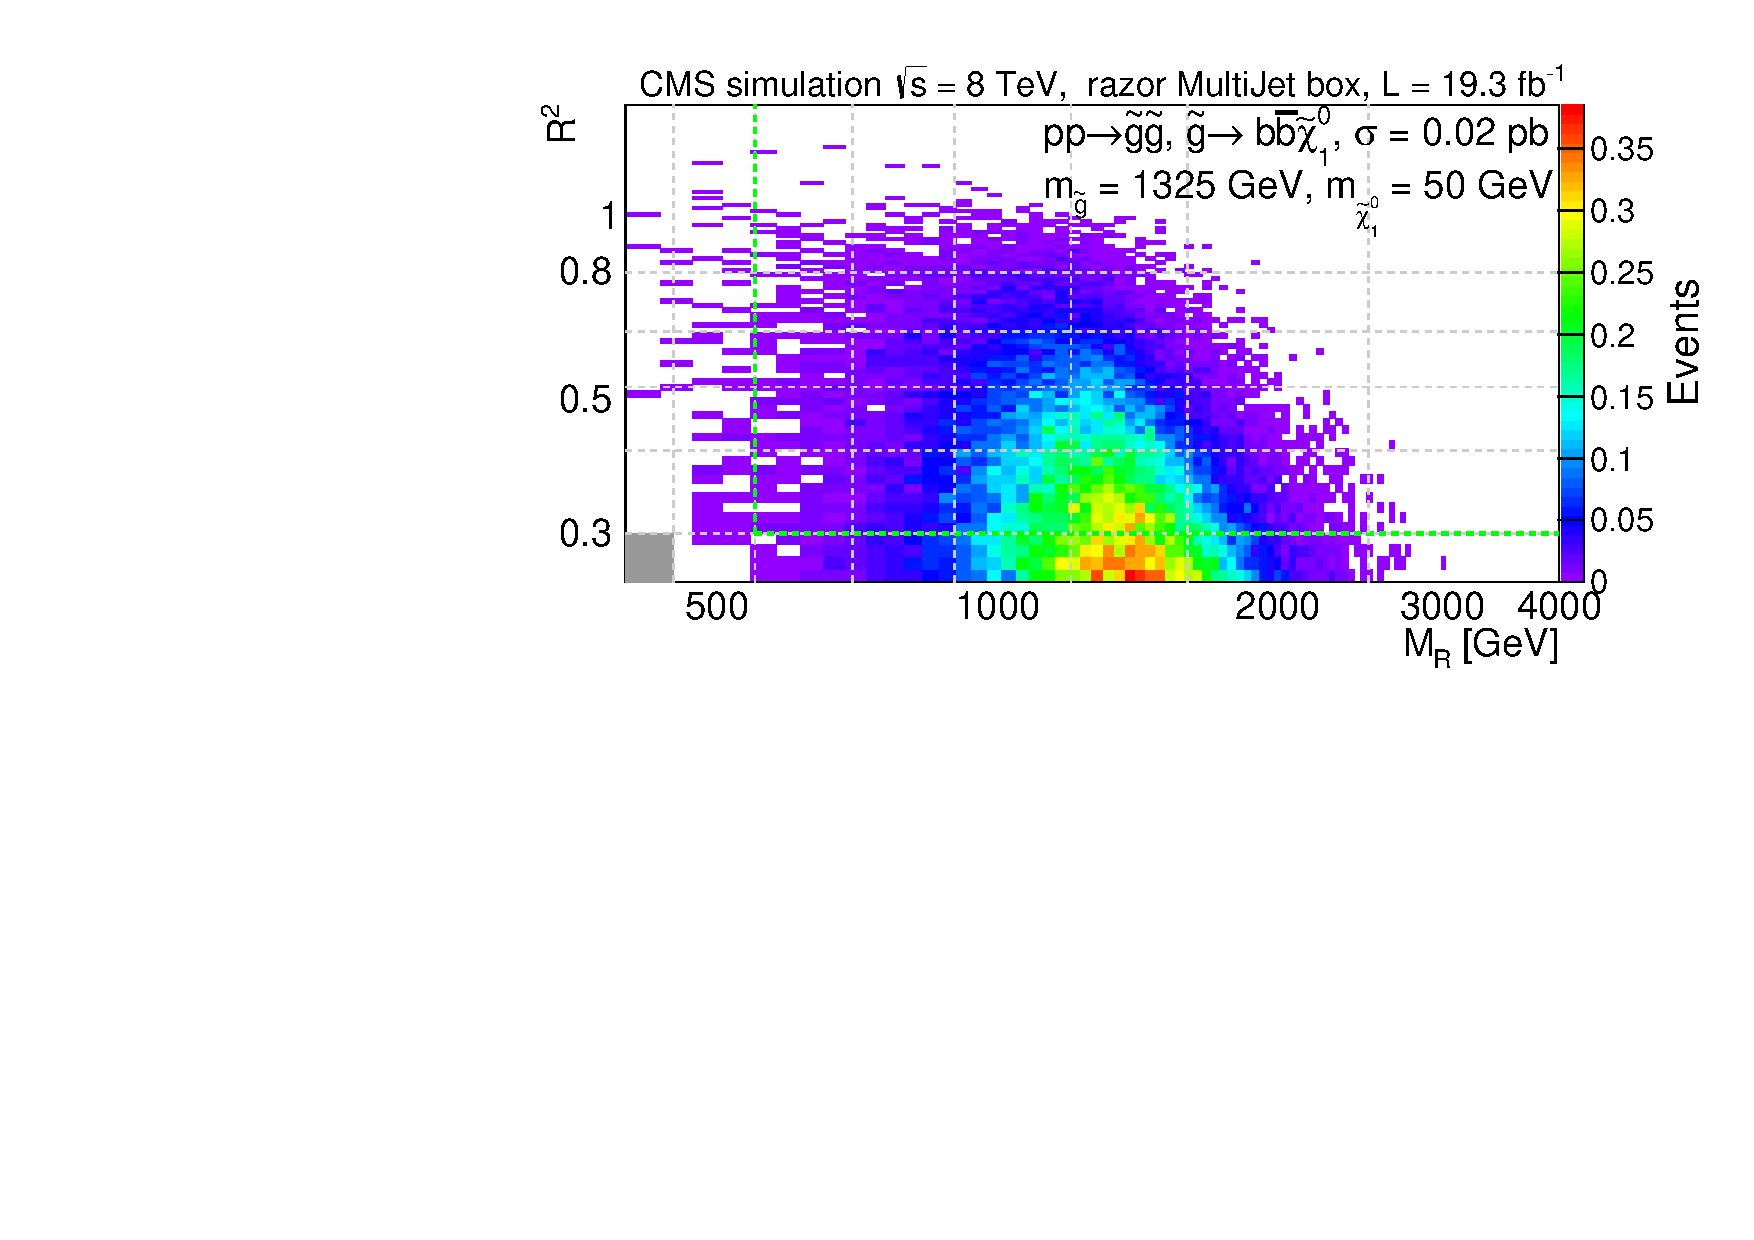
\includegraphics[width=0.49\textwidth]{figs/analysis8TeV/T1bbbb_1325_50_FF.pdf}
\caption{Distribution of (left) simulated SM background events and (right)
  T1bbbb gluino-gluino events in the MultiJet box. Each $\sGlu$ is
  forced to decay to a \bbbar pair and a $\chiz_1$,
  assumed to be the stable LSP. The $\sGlu$ and $\chiz_1$ masses are
  fixed to 1325\GeV and 50\GeV,
  respectively.\label{fig:T1bbbbsignalinj}}

\end{figure}

\begin{figure}[htb!]
\centering
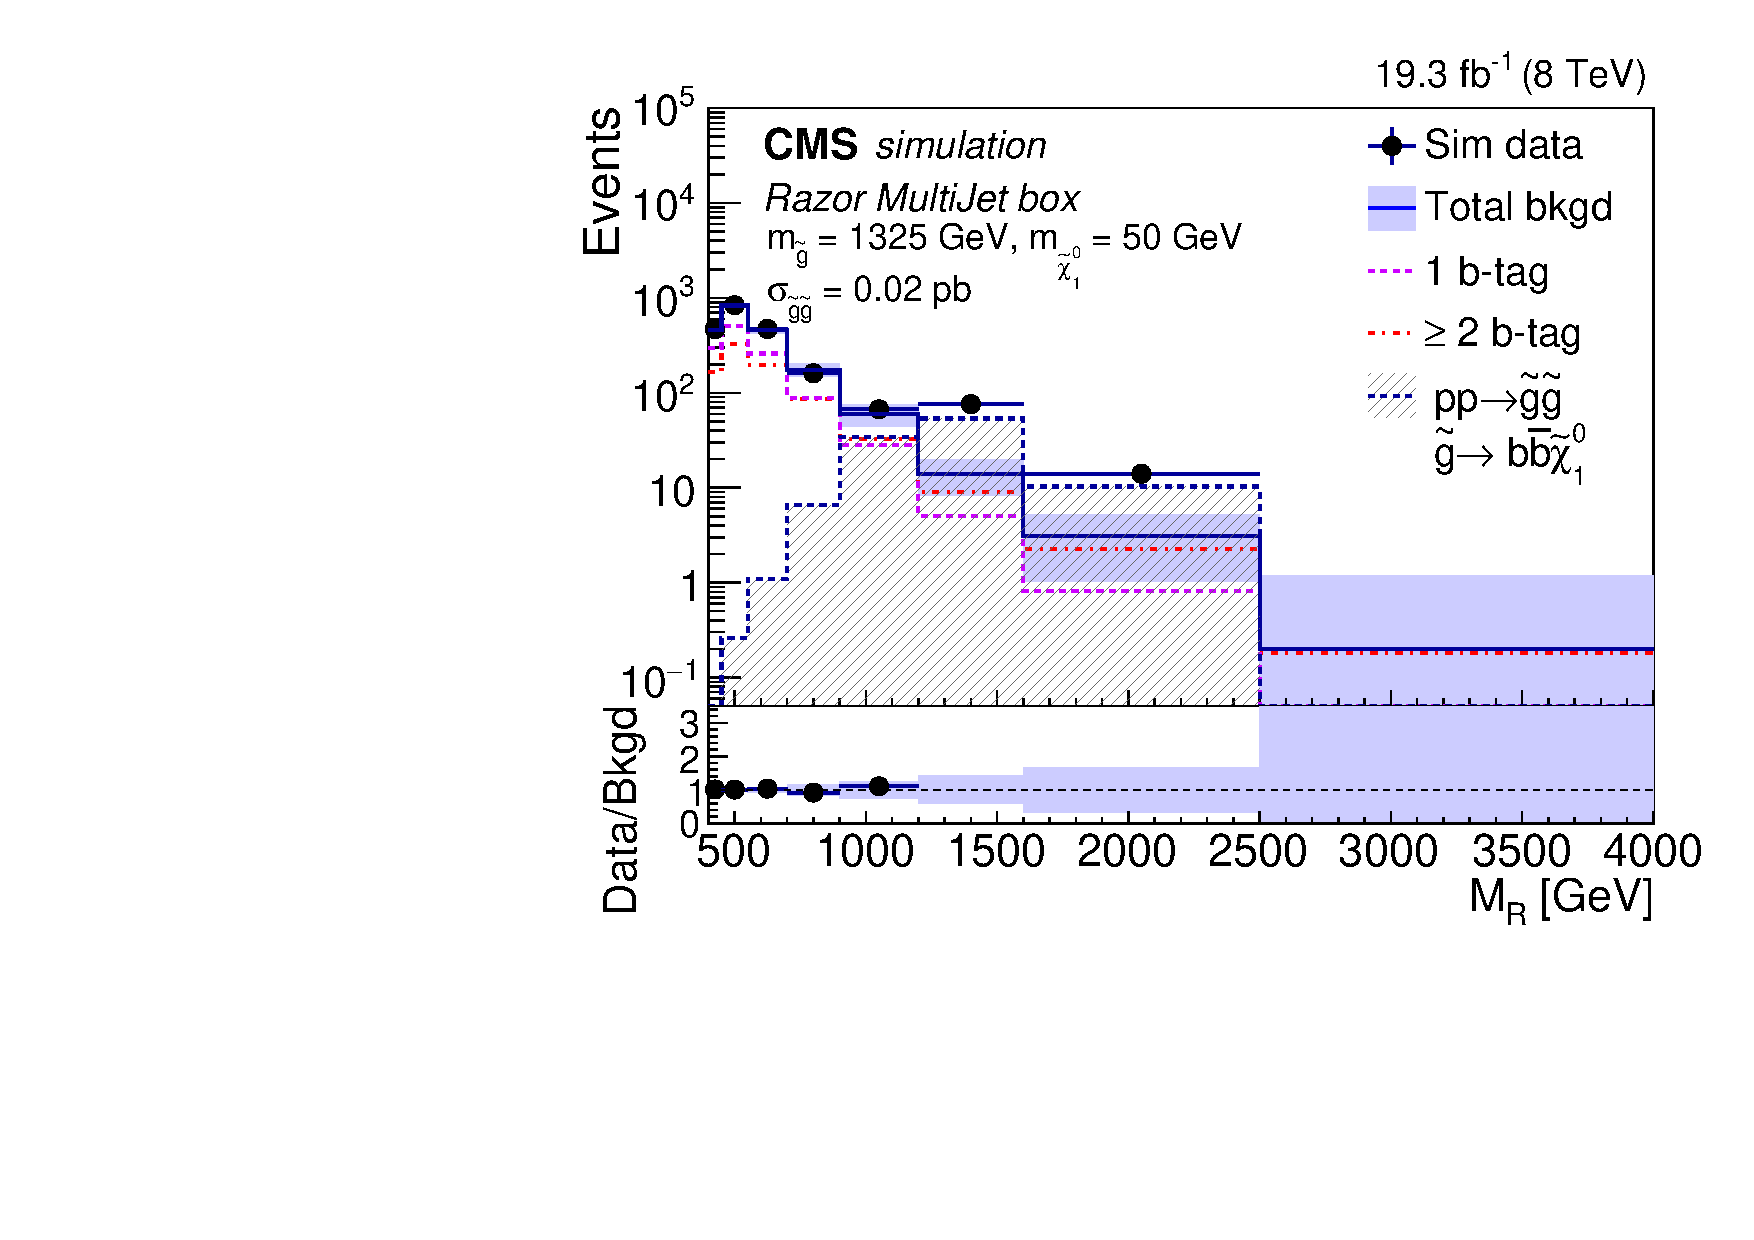
\includegraphics[width=0.49\textwidth]{figs/analysis8TeV/MR_T1bbbb_0p02_MultiJet.pdf}
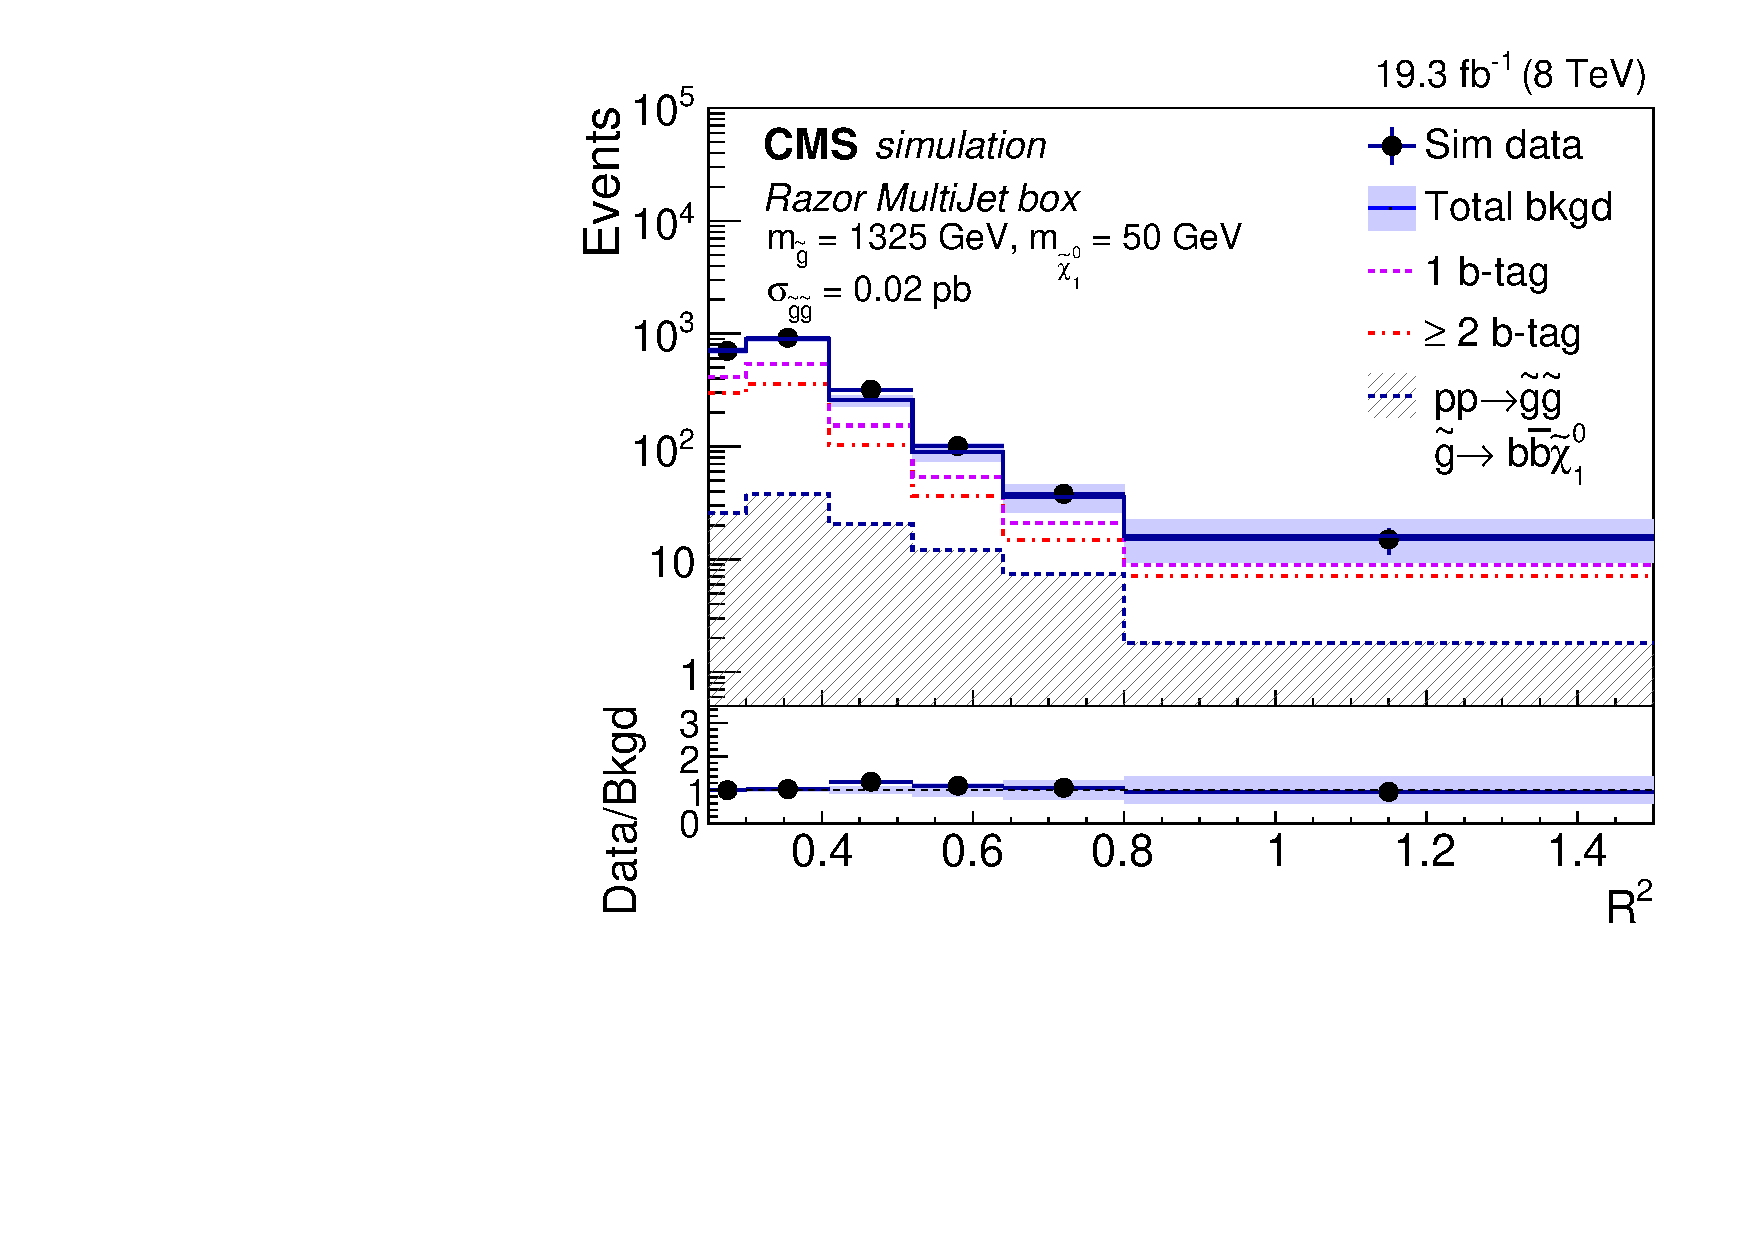
\includegraphics[width=0.49\textwidth]{figs/analysis8TeV/RSQ_T1bbbb_0p02_MultiJet.pdf}
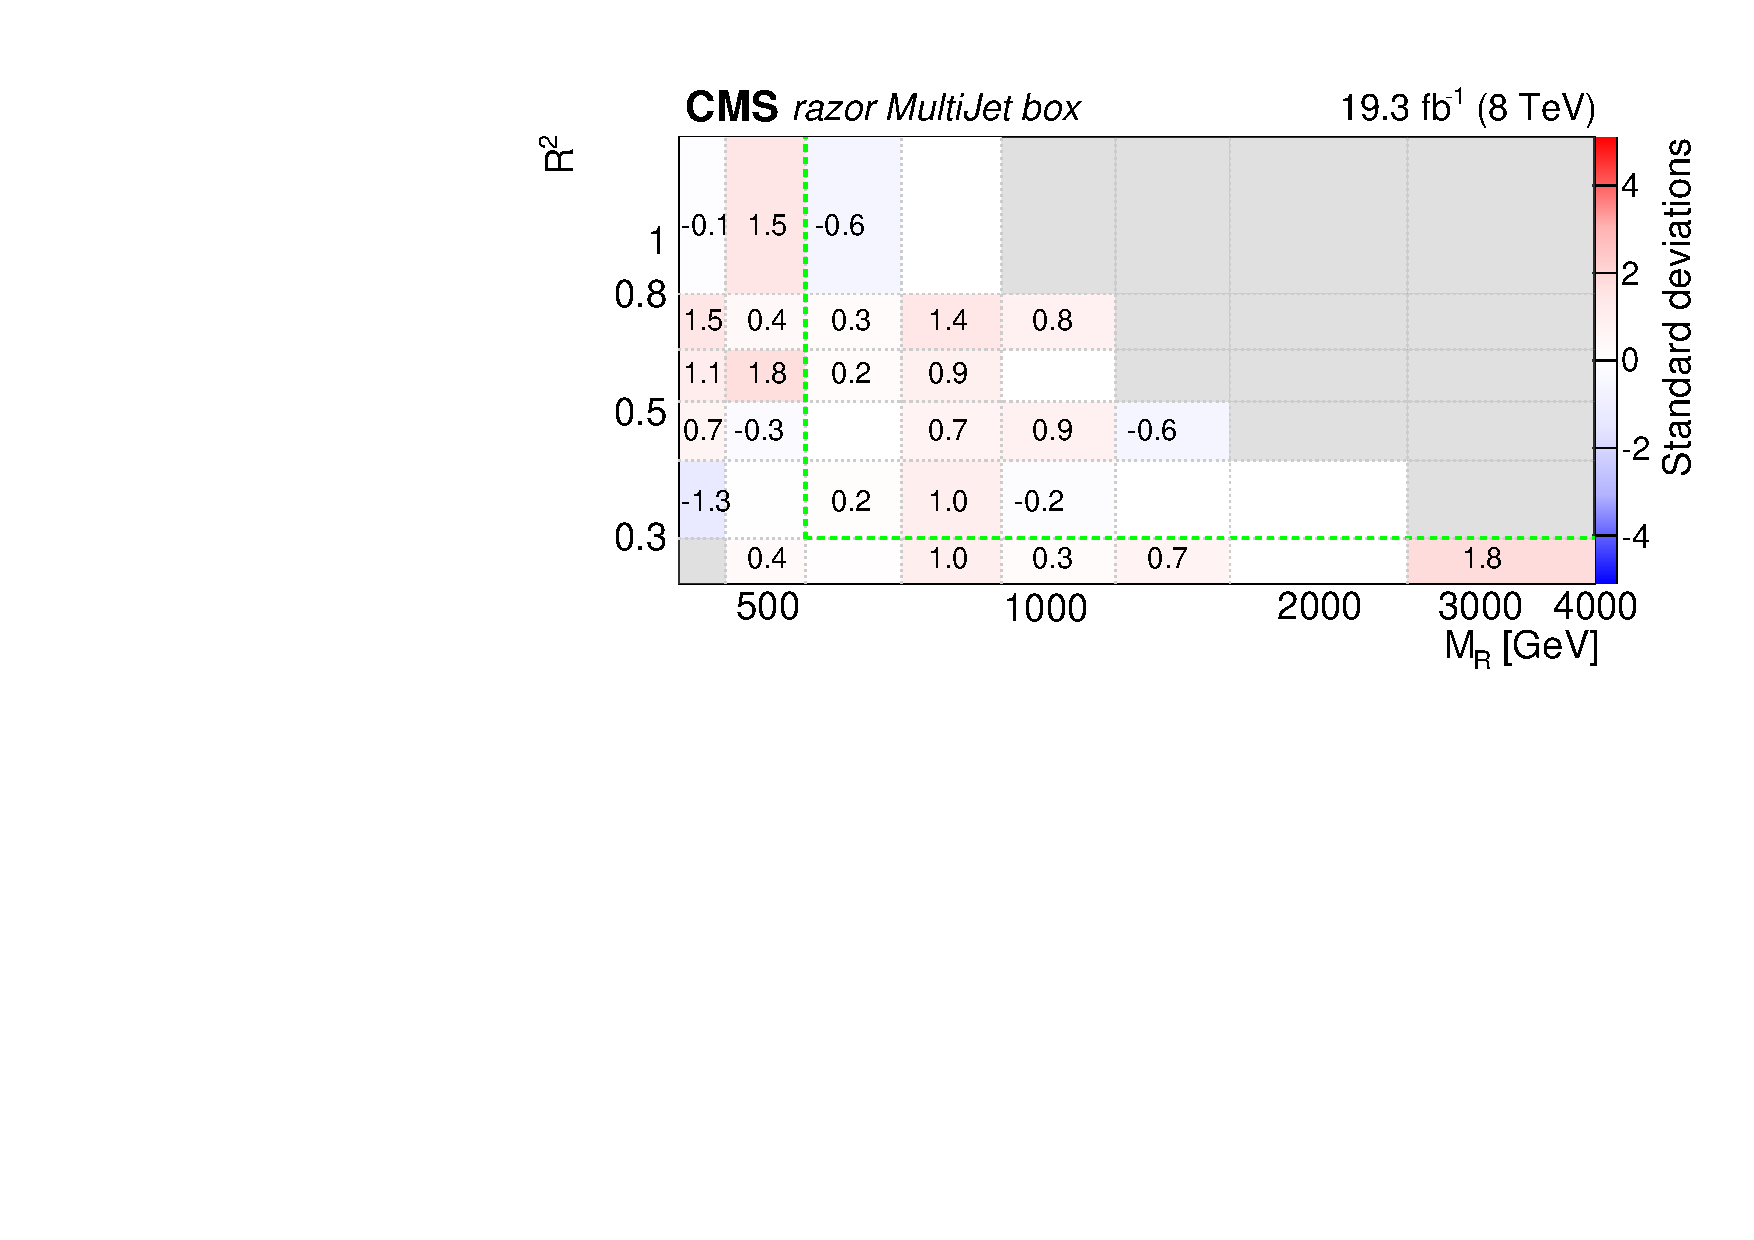
\includegraphics[width=0.49\textwidth]{figs/analysis8TeV/nSigmaLog_MultiJet.pdf}
\caption{Result of the fit to the sideband events of a
  signal-plus-background MC sample, corresponding to the gluino model
  whose distribution is shown in Fig.~\ref{fig:T1bbbbsignalinj}. A
  gluino-gluino production cross section of 0.02\unit{pb} is assumed. The
  one-dimensional projections on (upper left) \MR and (upper right)
   \Rtwo are shown, together with (bottom) the agreement between
  the observed yield and the prediction from the sideband fit as a
  function of  \Rtwo and $\MR$. This agreement is
  evaluated from a two-sided p-value using an ensemble of
  background-only pseudo-experiments as described in
  Section~\ref{sec:bmodel}.\label{fig:FFsigma0p02}}
\end{figure}


\section{Limit-setting procedure}
\label{sec:limit}


We interpret the results of the searches by determining the 95\%
confidence level (\CL) upper limits on the production cross sections of
the SUSY models presented in Section~\ref{sec:sms}, using the LHC
\CLs procedure~\cite{LHCCLs} and a global likelihood
determined by combining the likelihoods of the different search boxes
and sidebands.  To reduce computational requirements, a binned
likelihood is used, 
\begin{equation}
\mathcal L(\mathrm{data}|\mu,\boldsymbol{\theta})=\prod_{i=1}^{n_b} \mathrm{Poisson}(x_i|s_i(\mu,\boldsymbol{\theta})+b_i(\boldsymbol{\theta}))\cdot \mathrm{Constraint}(\boldsymbol{\theta}|\boldsymbol{\bar\theta},\boldsymbol{\delta\theta})~,
\end{equation}
where $\mu$ is the signal strength (parameter of interest),
$\boldsymbol{\theta}$ is the vector of nuisance parameters, $x_i$ is
the data yield in the $i$th bin, $s_i(\mu,\boldsymbol{\theta})$ the
corresponding signal yield, $b_i(\boldsymbol{\theta})$ the
corresponding background yield, computed as
\begin{equation}
b_i(\boldsymbol{\theta}) = N_{\mathrm{SM}} \int^{\MR^{\mathrm{max},i}}_{\MR^{\mathrm{min},i}}
  \int^{\Rtwo_{\mathrm{max},i}}_{\Rtwo_{\mathrm{min},i}} P_{\mathrm{SM}}(\MR,\Rtwo)  \mathrm{d}\Rtwo \mathrm{d}\MR ~,
\end{equation}
and the product runs over $n_b$, the
number of bins. This then is used to define the test statistic
following the LHC \CLs procedure,
\begin{equation}
\tilde q_{\mu} = -2\log\frac{\mathcal L(\mathrm{data}|\mu,\boldsymbol{\hat\theta}_{\mu})}{\mathcal L(\mathrm{data}|\hat\mu, \boldsymbol{\hat\theta})} ~,~~  0\leq\hat\mu\leq\mu~.
\end{equation}

For the razor search boxes, the signal contribution is modeled by a
template function, for a given signal hypothesis in a specific box and
a given \PQb-tagged jet multiplicity. The template function, normalized
to unit probability, is multiplied by the expected signal yield in
each bin ($\sigma_\mathrm{NLO+NLL} L
\epsilon^{\text{box}}_{\PQb\text{-tag}}$). Here $\sigma_\mathrm{NLO+NLL}$ is
the SUSY signal cross section, $L$ is the integrated luminosity
corresponding to the size of the data set, and
$\epsilon^{\text{box}}_{\PQb\text{-tag}}$ is the signal selection
efficiency for a given box and, in case of the single-lepton and
hadronic boxes, for a given \PQb-tagged jet multiplicity.

Each systematic uncertainty is incorporated in the likelihood with a
dedicated nuisance parameter, whose value is not known a priori but
rather must be estimated from the data. The set of nuisance parameters
may be divided into three distinct classes (though their statistical
treatment is the same): those related to the signal normalization,
those related to the signal shape, and those related to the background
normalization and shape.

We consider the following systematic uncertainties associated with the
signal normalization, with the size of the uncertainty indicated in
parentheses:
\begin{itemize}
\item integrated luminosity (2.6\%)~\cite{CMS:2013gfa};
\item trigger efficiency (5\%);
 \item lepton reconstruction and identification efficiencies (3\%
  per lepton), measured from an inclusive $\cPZ\to \ell^+\ell^-$ event
  sample ($\ell=\Pe,\Pgm$) as a function of the lepton $\pt$ and $\eta$
  values~\cite{Chatrchyan:2013iaa,Chatrchyan:2013mxa}.
\end{itemize}

In addition, four signal-shape systematic uncertainties are considered, whose
sizes vary with $\Rtwo$, $\MR$, and the \PQb-tagged jet
multiplicity:
\begin{itemize}
\item The uncertainty in the jet \PQb-tagging and mistagging efficiencies
  (up to 20\% depending on the signal model), evaluated for each
  ($\MR$, $\Rtwo$) and \PQb-tagged jet multiplicity
  bin. The uncertainty is evaluated by propagating the uncertainty in
  data-to-simulation scale factors~\cite{btag8TeV}.
\item the uncertainty in the modeling of the parton distribution
  functions (PDFs) (up to 10\% depending on the signal model),
  evaluated for each bin in the ($\MR$, $\Rtwo$) plane
  and for each box and \PQb-tag multiplicity following the
  PDF4LHC~\cite{Bourilkov:2006cj,Alekhin:2011sk,Botje:2011sn}
  prescription, using the CTEQ-6.6~\cite{Nadolsky:2008zw} and
  MRST-2006-NNLO~\cite{Martin:2007bv} PDF sets.
\item The uncertainty in the jet energy scale and resolution (up to
  5\% depending on the signal model), evaluated from a set of data
  control samples and MC simulations~\cite{JME-JINST}.
\item The uncertainty in the modeling of the associated jet production
  by the \MADGRAPH simulation (up to 20\% depending on the
  signal model), studied using $\cPZ$+jets and $\ttbar$ data events
  and parameterized by an MC-to-data scale factor as a function of the
  magnitude of the vector sum of the $\pt$ values of the two produced
  SUSY particles~\cite{1LepMVA}.
\end{itemize}
The impact of each of these uncertainties on the SUSY signal shape is
taken into account by varying each effect up or down by one standard
deviation.

The uncertainty in the knowledge of the background distributions
is taken into account by maximizing the likelihood with respect to the background shape and
normalization parameters using the data in the two
sidebands and the signal-sensitive region. The background parameterization
is able to accommodate several sources of
systematic uncertainties defined below:
\begin{itemize}
\item dependence of the background shape on the \PQb-tag multiplicity;
\item dependence of the background shape on the lepton and jet
 multiplicities;
\item deviation of the two-dimensional shape from an exponentially falling
 distribution, through the background empirical function parameter $n$,
 which modifies the tail in \MR and $\Rtwo$;
\item shape bias induced by the dependence of the \PQb-tagging efficiency and
 mistag rate on the jet $\pt$;
\item deviation of the \PQb-tagging and mistagging efficiencies from the
 MC prediction, through independent normalization factors in each
 \PQb-tagged jet multiplicity bin.
\end{itemize}



The combination of razor and exclusive single-lepton~\cite{1LepMVA}
searches is performed using the same procedure, taking into account
the systematic uncertainties associated with the five following
effects:
\begin{itemize}
\item the PDFs;
\item the jet energy scale correction;
\item the integrated luminosity;
\item the b-jet tagging efficiency;
\item the associated jet production.
\end{itemize}
The uncertainties in the background predictions are taken to be
uncorrelated, being derived from independent data control samples with
different techniques. We verified that the correlation model for the
systematics has a negligible impact on the combination, since similar
results are obtained when neglecting any correlation between the
systematic uncertainties of the two searches.

\section{Interpretation}
\label{sec:interp}

The results of this search are interpreted in the context of the natural
SUSY simplified models presented in Section~\ref{sec:sms}.

\subsection{Limits on gluino pair production}
\label{sec:interp:gluino}

Derived limits on gluino pair production in the T1bbbb, T1tbbb,
T1ttbb, T1tttb, and T1tttt scenarios are presented in
Fig.~\ref{fig:gluino2D}.  A comparison of the simplified natural SUSY
gluino-gluino exclusions, obtained for the different decay-mode
combinations of third generation quarks, is shown in
Fig.~\ref{fig:gluinogluinoSUMMARY}. The limits corresponding to
gluino-gluino topologies with mixed branching fractions lie within the
band defined by the T1bbbb and the T1tttt contours. As an example,
gluino masses smaller than 1175\GeV for T1tttt and 1310\GeV for T1bbbb
are excluded, for an LSP mass of 100\GeV. For any LSP mass value, a
larger number of top quarks in the decay topology corresponds to a
weaker limit, mainly due to a reduced total signal efficiency with
respect to the four-bottom-quark final state and a worse \MR and
$\Rtwo$ resolution for events with higher jet multiplicity in the
final state. Given this fact and the inclusive nature of the analysis,
the T1tttt limit can be considered to represent a conservative
estimate of a branching-fraction-independent limit, generically valid
for gluino-gluino production within the context of the natural SUSY
spectrum shown in Fig.~\ref{fig:spectrum}.

\begin{figure*}[t]
\centering
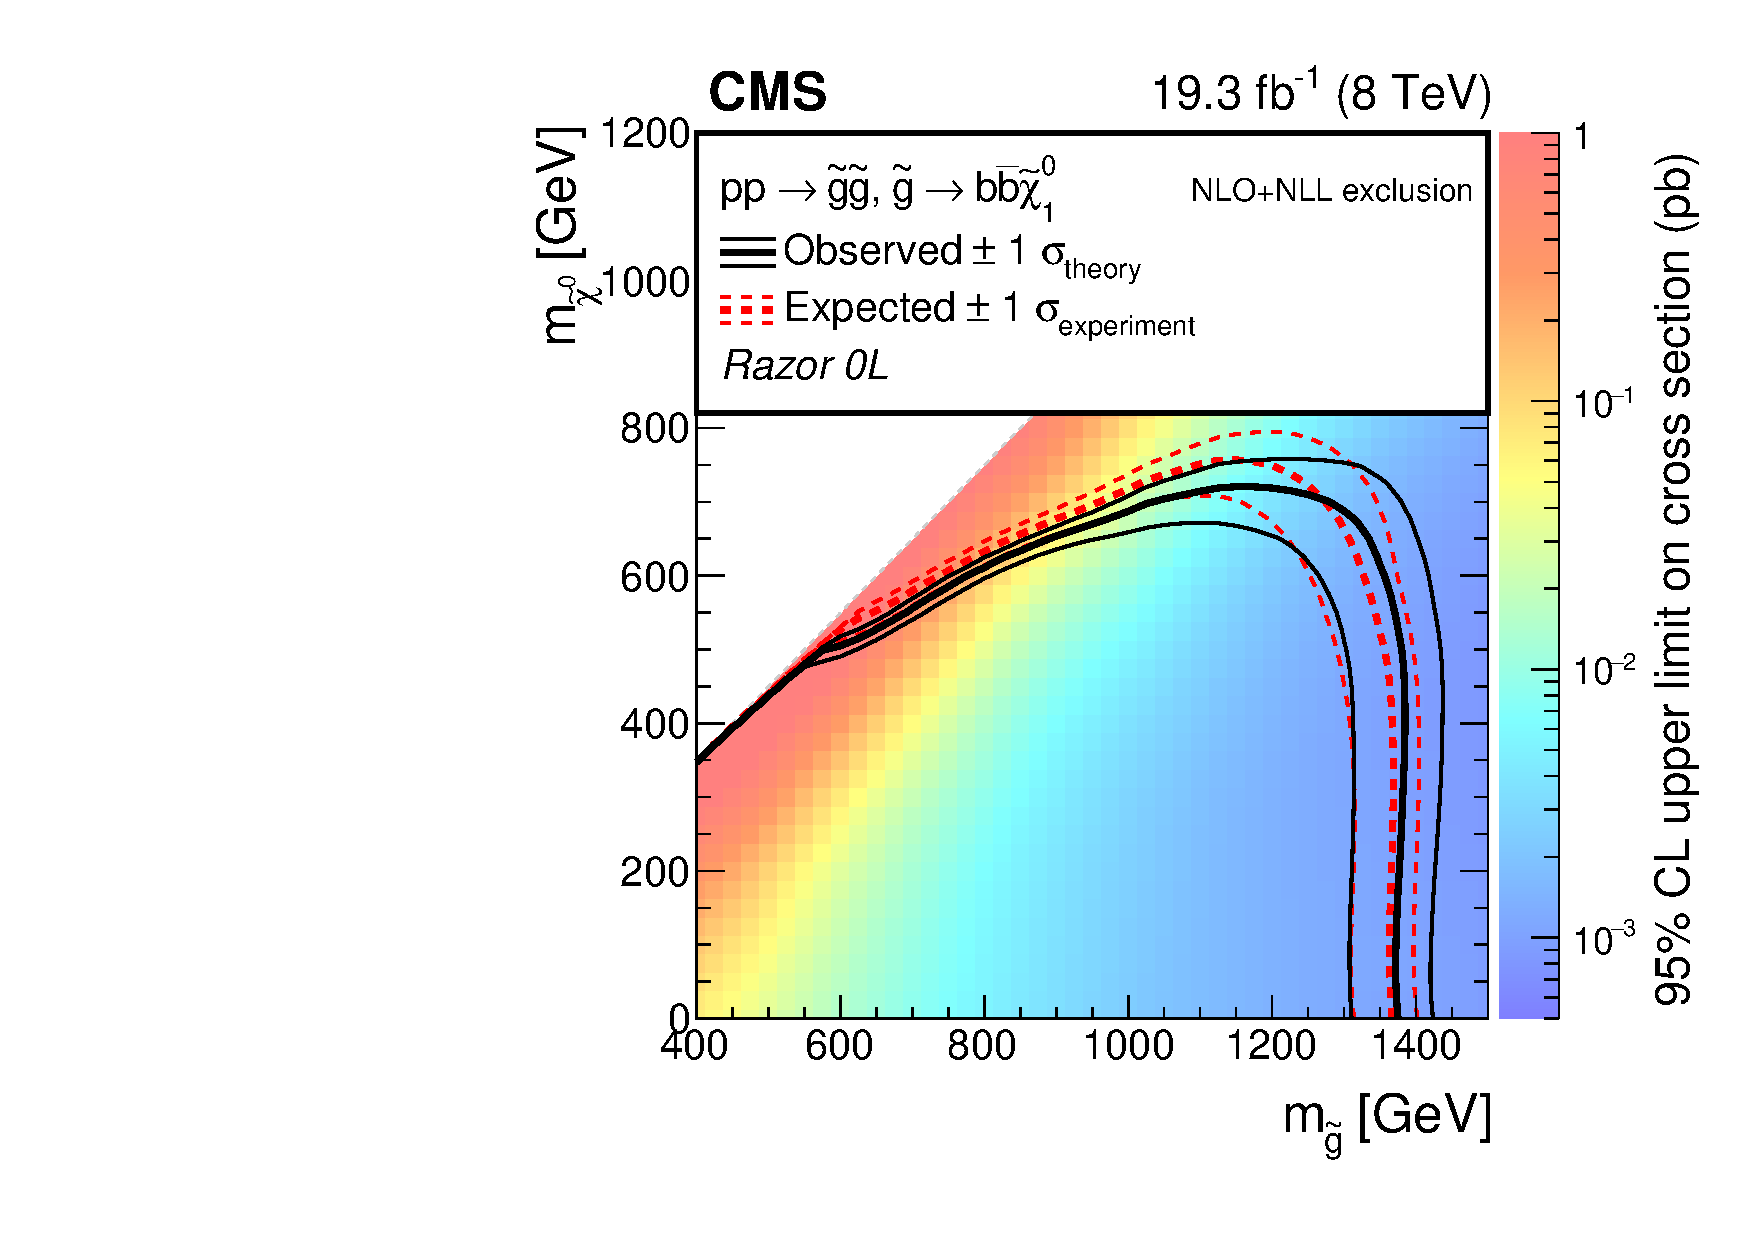
\includegraphics[width=0.4\textwidth]{figs/analysis8TeV/T1bbbbHybridNew0LXSEC.pdf}
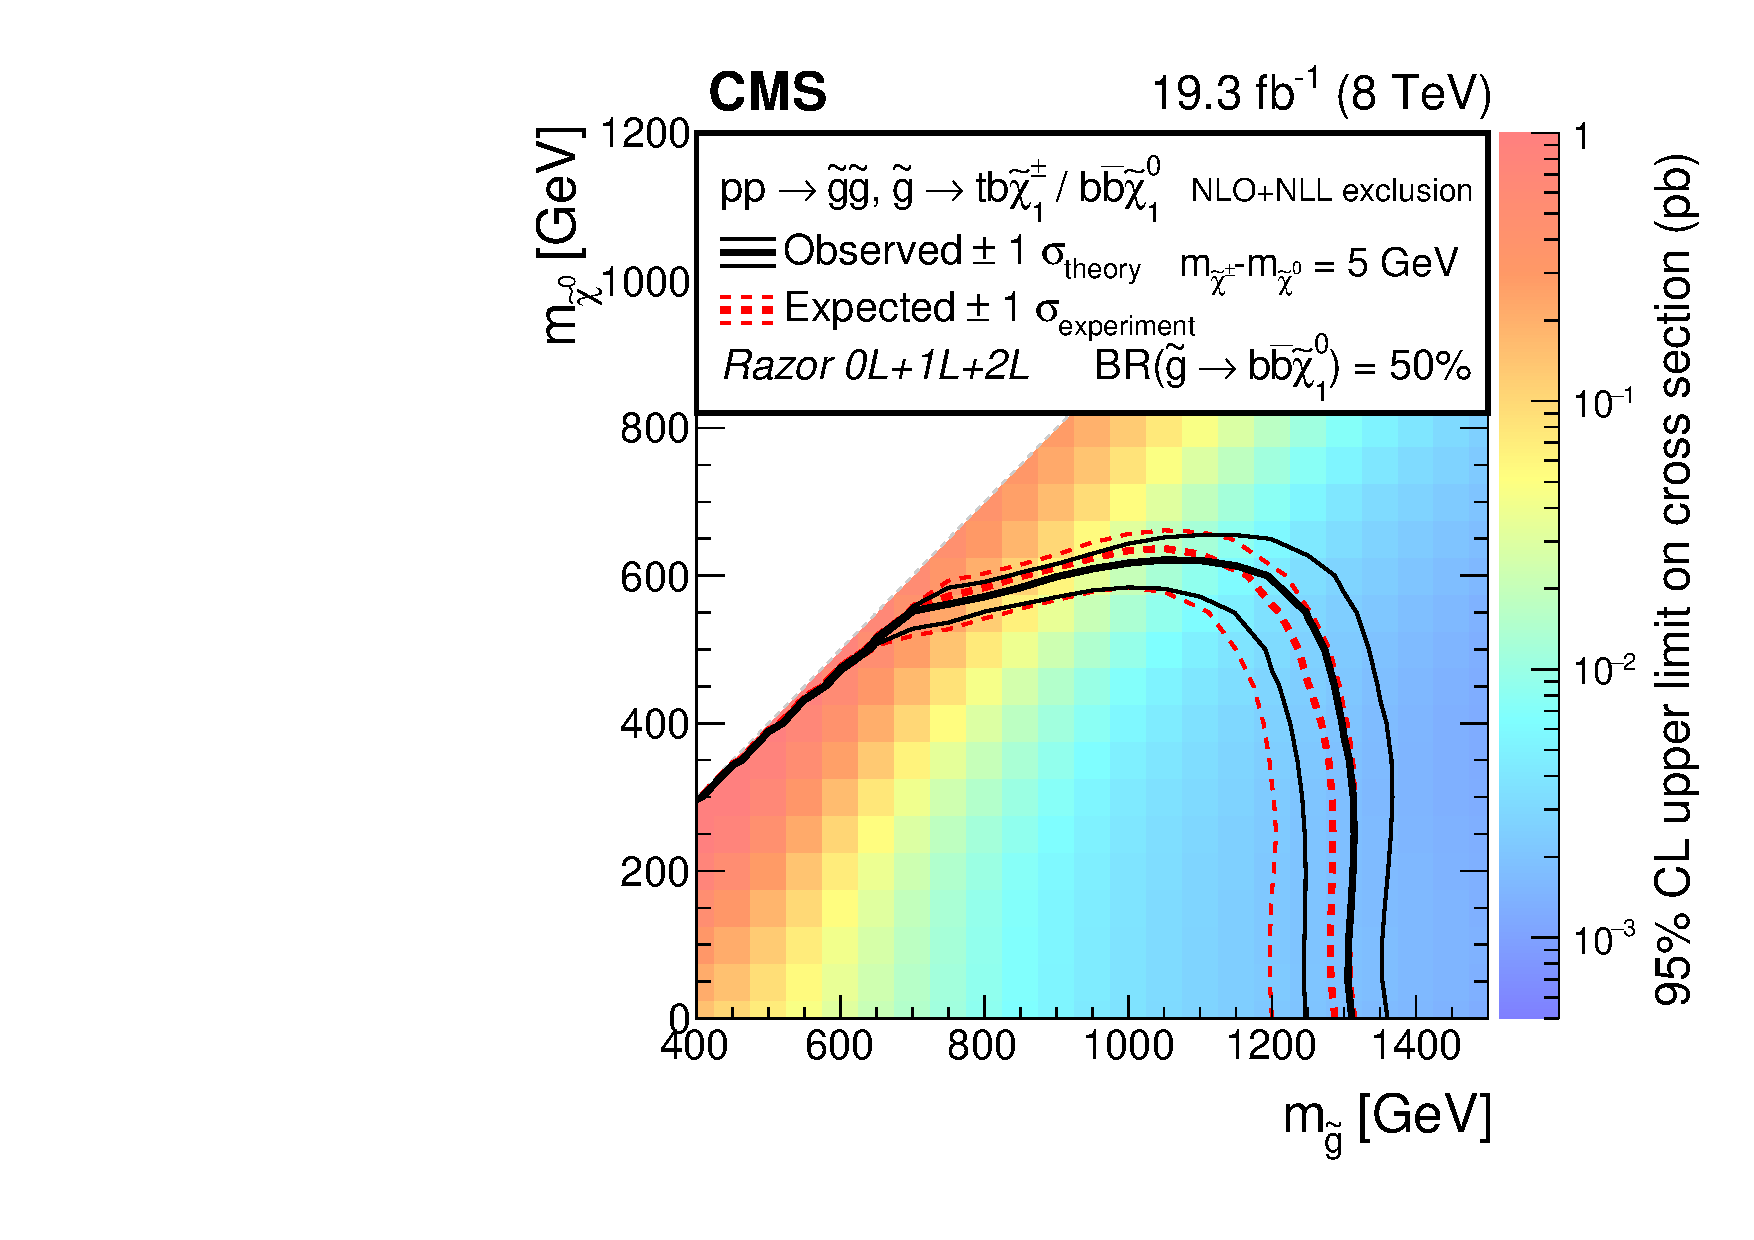
\includegraphics[width=0.4\textwidth]{figs/analysis8TeV/T1tbbbHybridNew0Lp1Lp2LXSEC.pdf}
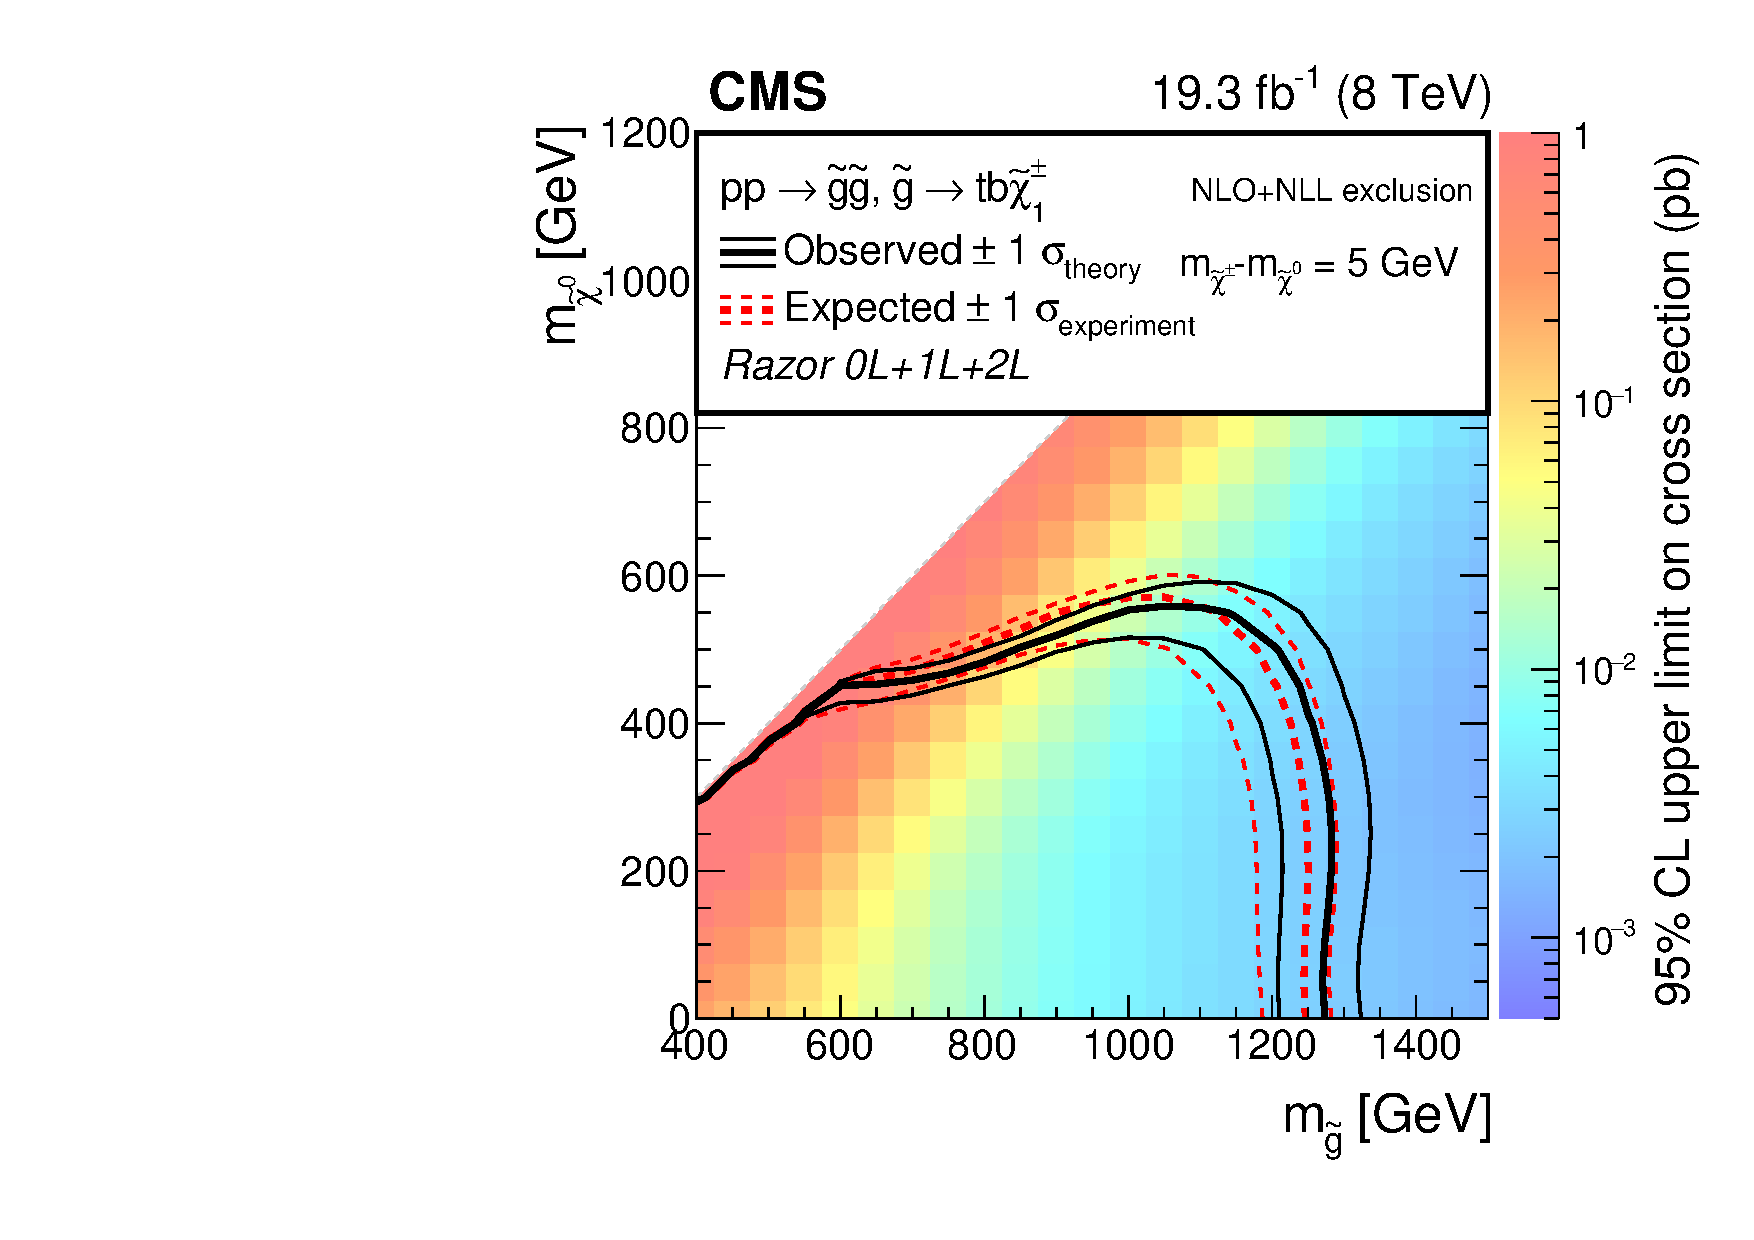
\includegraphics[width=0.4\textwidth]{figs/analysis8TeV/T1ttbbHybridNew0Lp1Lp2LXSEC.pdf}
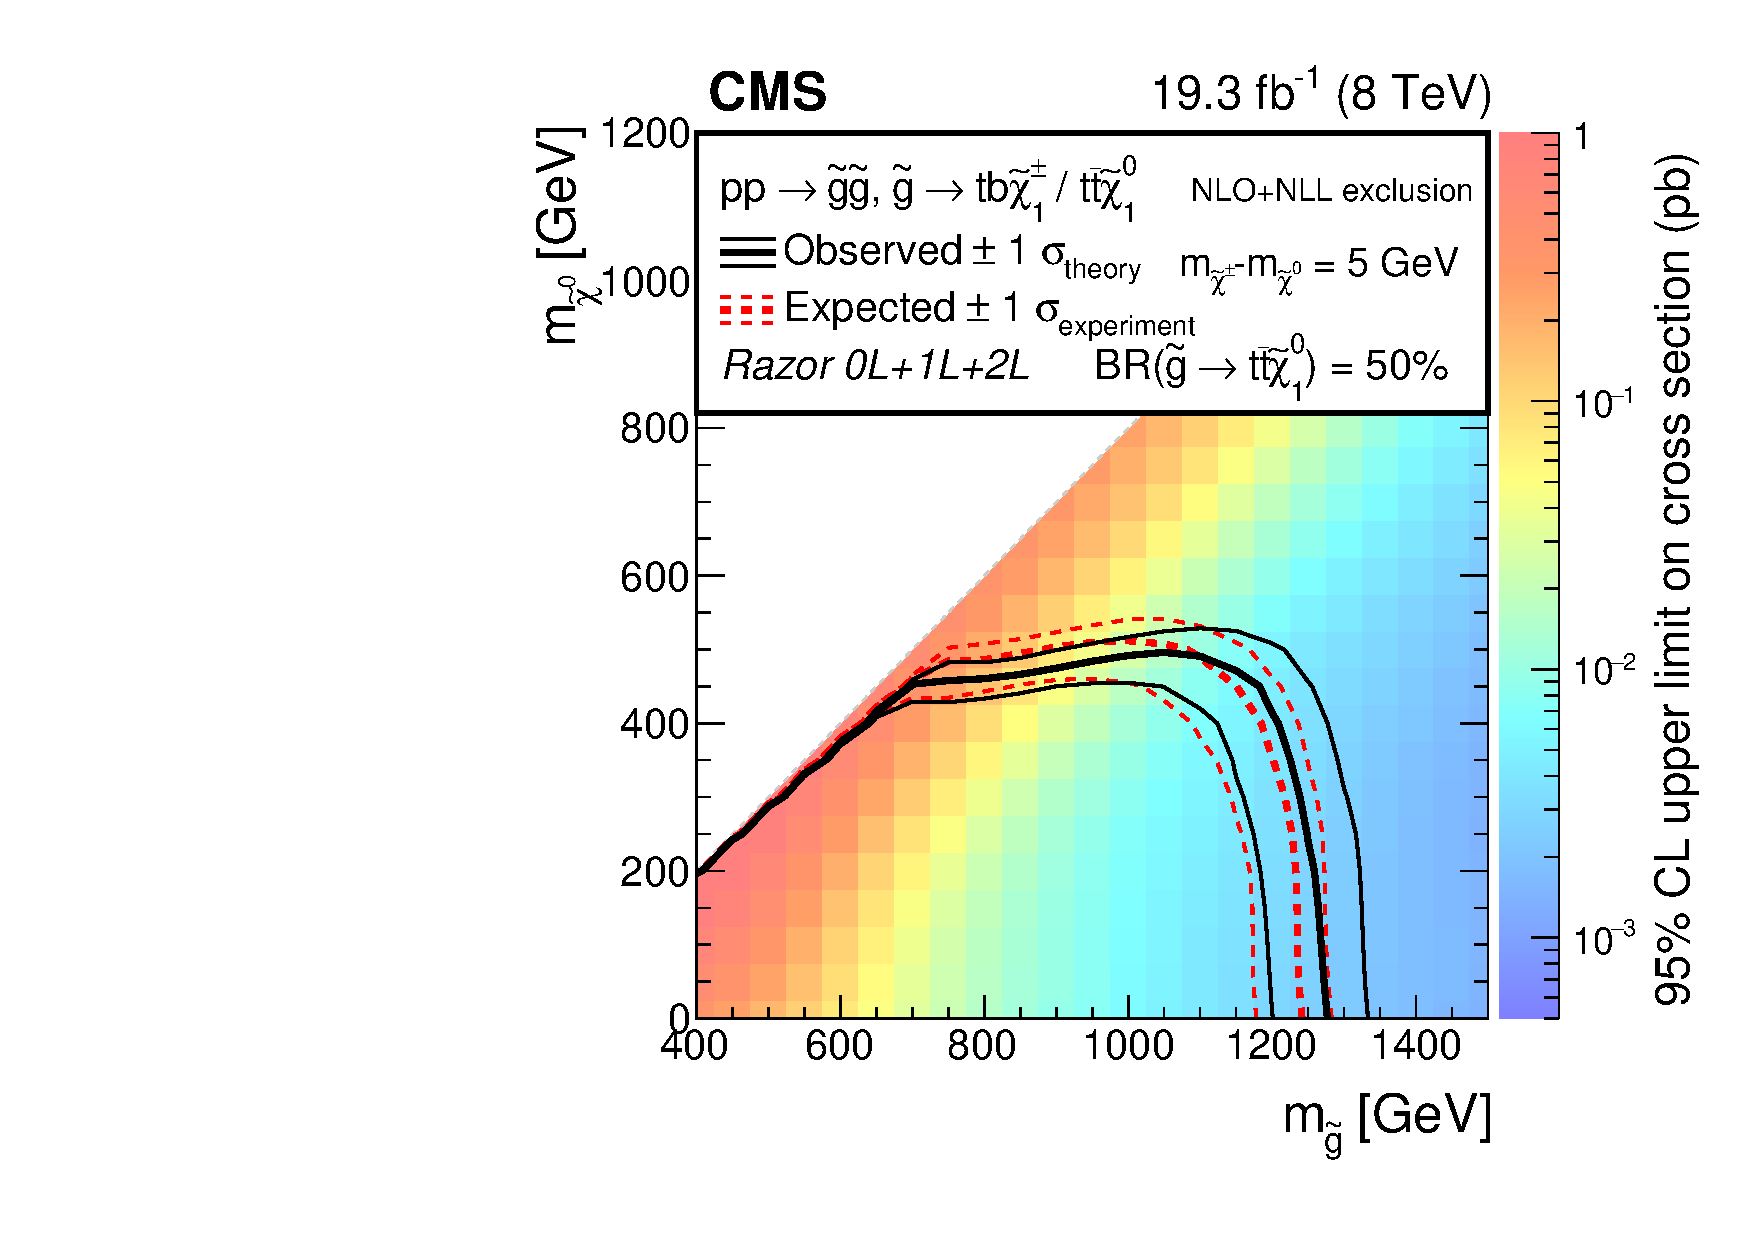
\includegraphics[width=0.4\textwidth]{figs/analysis8TeV/T1tttbHybridNew0Lp1Lp2LXSEC.pdf}
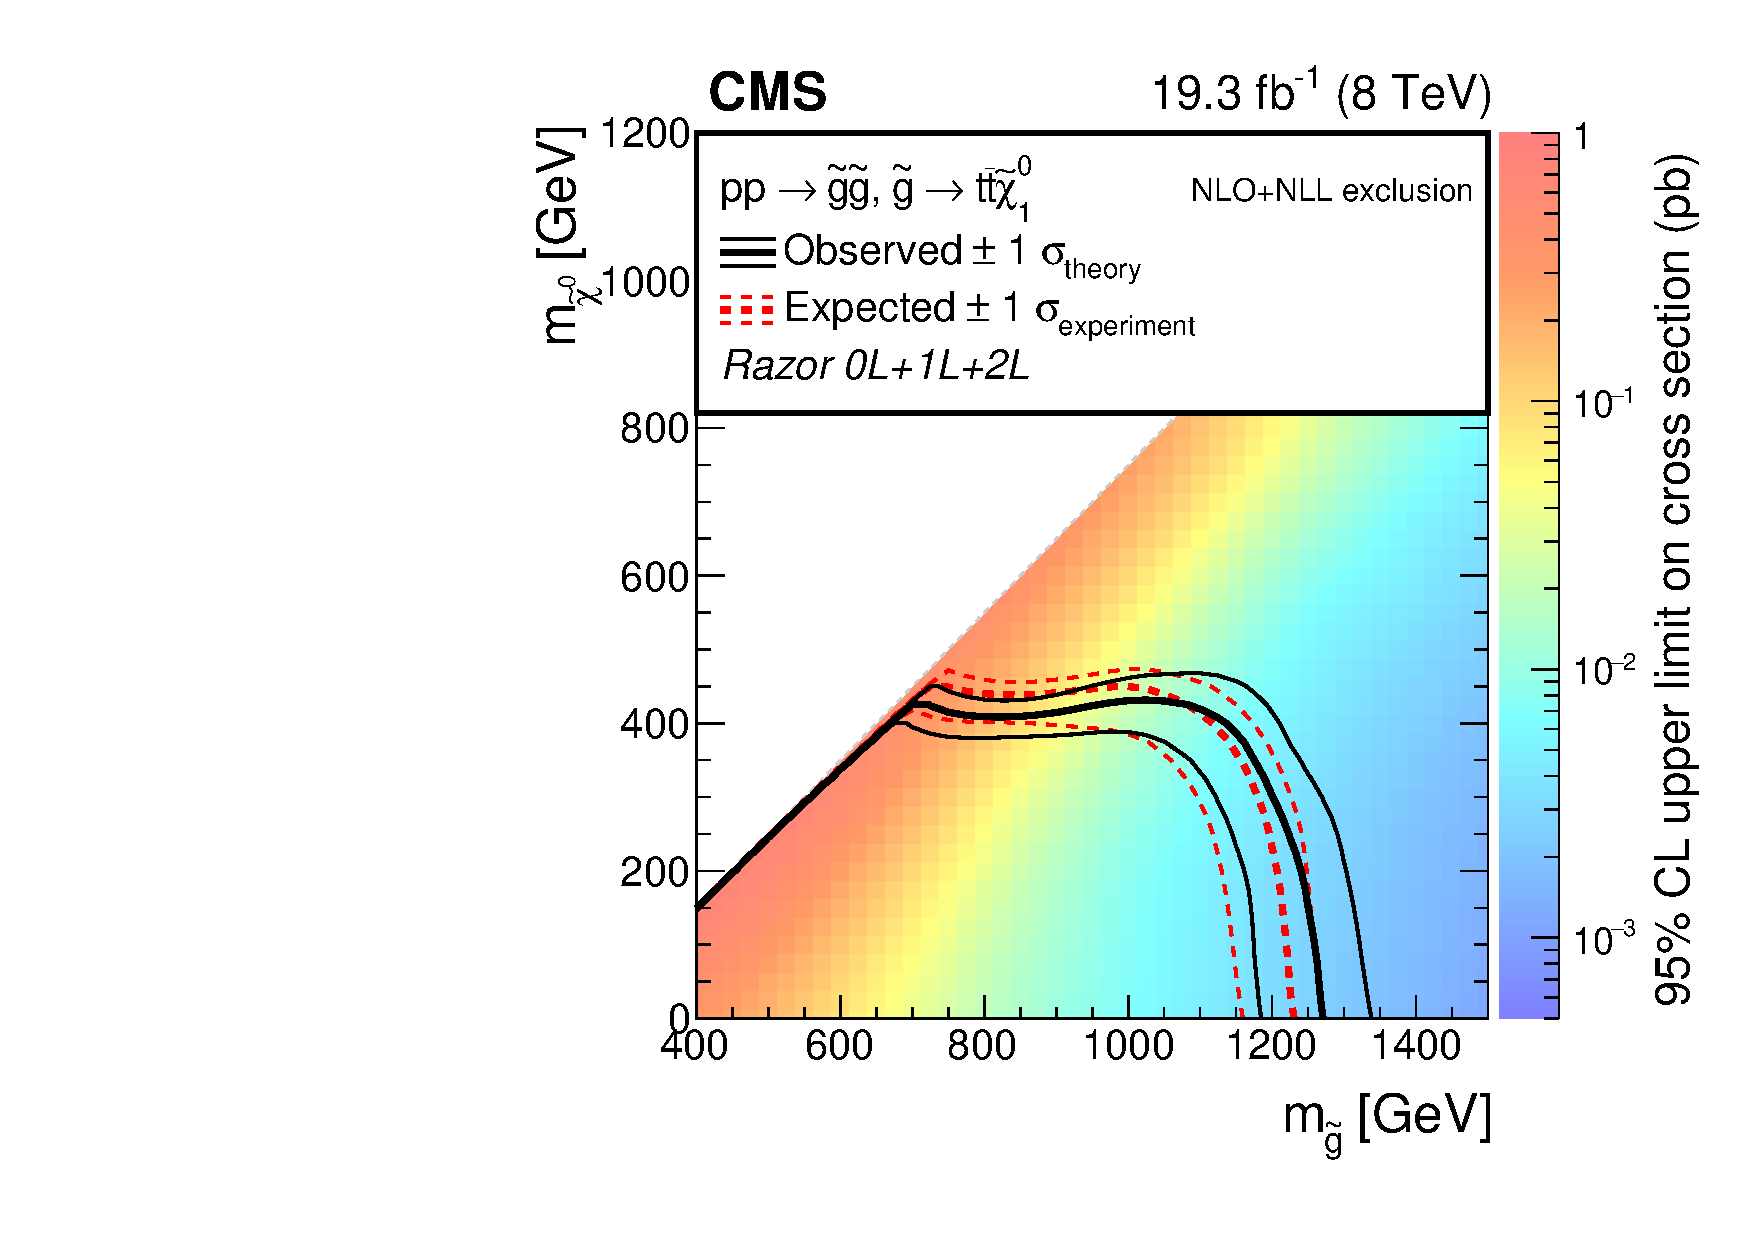
\includegraphics[width=0.4\textwidth]{figs/analysis8TeV/T1ttttHybridNew0Lp1Lp2LXSEC.pdf}
\caption{Interpretation of the inclusive search with razor variables
  in the context of gluino pair production models: (upper left) T1bbbb, (upper right)
  T1tbbb, (middle left) T1ttbb, (middle right) T1tttb, and (bottom) T1tttt. The limit for T1bbbb
  is derived using only the hadronic boxes, while the limits for the
  remaining models are derived using all nine boxes. The color coding
  indicates the observed 95\% \CL upper limit on the signal cross
  section. The dashed and solid lines represent the expected and
  observed exclusion contours at a 95\% \CL, respectively. The dashed
  contours around the expected limit and the solid contours around the
  observed one represent the one standard deviation theoretical
  uncertainties in
  the cross section and the combination of the statistical and
  experimental systematic uncertainties,
  respectively.\label{fig:gluino2D}}
\end{figure*}

\begin{figure}[tb!]
\centering
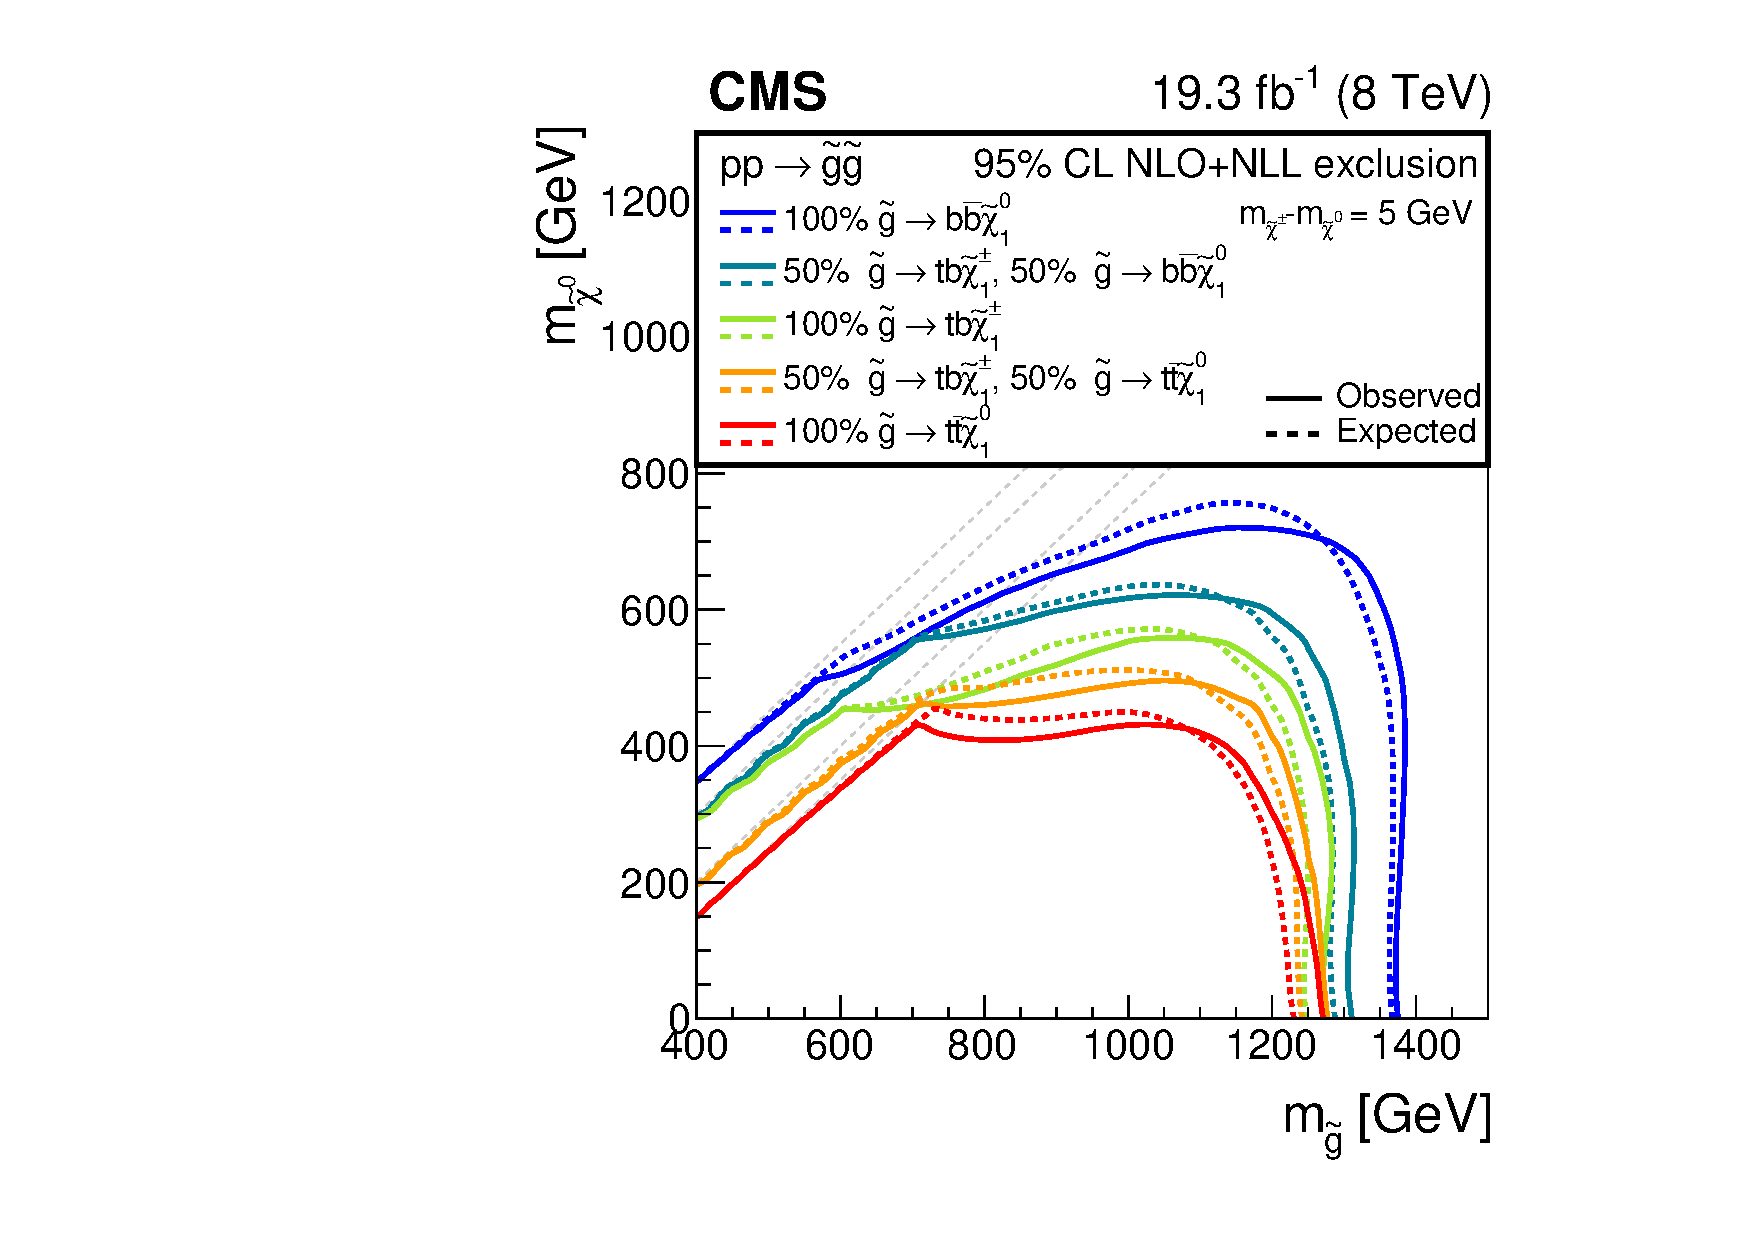
\includegraphics[width=\cmsFigWidth]{figs/analysis8TeV/T1HybridNew0Lp1Lp2LBARE.pdf}
\caption{Gluino mass limit at a 95\% \CL, obtained for different gluino
  pair production models with the inclusive razor analysis in the
  context of the natural SUSY spectrum of
  Fig.~\ref{fig:spectrum}.\label{fig:gluinogluinoSUMMARY}}

\end{figure}



\subsection{Limits on top-squark pair production}
\label{sec:interp:stop}

Derived limits on squark pair production from the razor variables in
the T2bW$^{\ast}$, T2tb, and T2tt scenarios are presented in
Fig.~\ref{fig:squark2D} and compared in
Fig.~\ref{fig:stopSUMMARY}. As in the
case of the gluino interpretation, the expected limit from the razor
search improves as the number of top quarks in the decay topology
decreases.
For an LSP mass of 100\GeV, top-squark mass values larger than
400\GeV and smaller than 650\GeV are excluded in all three
top-squark branching fraction scenarios.

Within the considered scenarios, a top-squark decay
to a chargino (neutralino) is topologically similar to a bottom-squark
decay to a neutralino (chargino). In the limit of degenerate charginos
and neutralinos, the decay products of the chargino are
generically too soft to be detected and this correspondence is
exact. However, for large mass differences between the squarks and the
chargino, the chargino decay products may be boosted enough to become
observable, breaking the correspondence. For the models
with the intermediate decay to charginos, there is a migration
of reconstructed events from the low-background 2b-Jet box to the
high-background MultiJet box and a consequently weaker
limit with respect to the simplified model without decays to charginos.

\begin{figure*}[tb!]
\centering
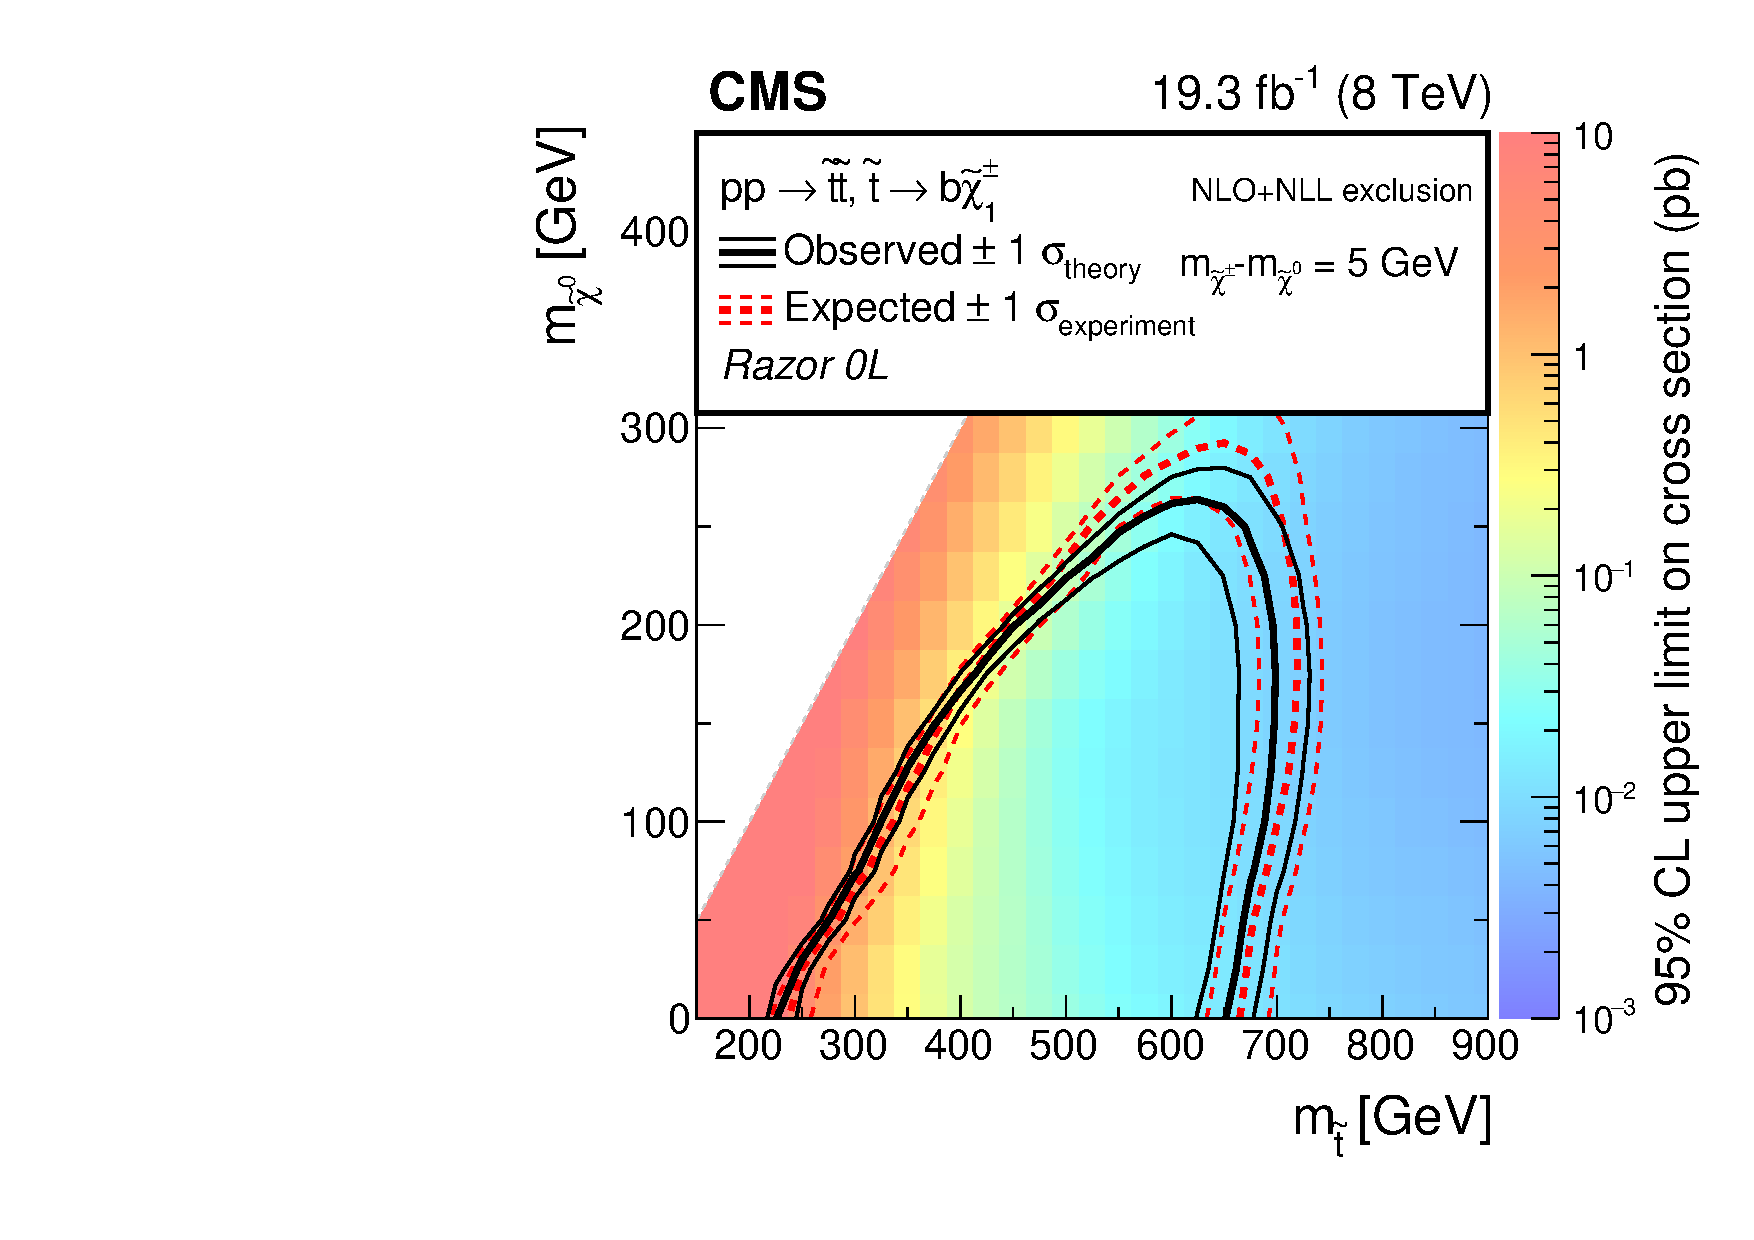
\includegraphics[width=0.49\textwidth]{figs/analysis8TeV/T2bwHybridNew0LXSEC.pdf}
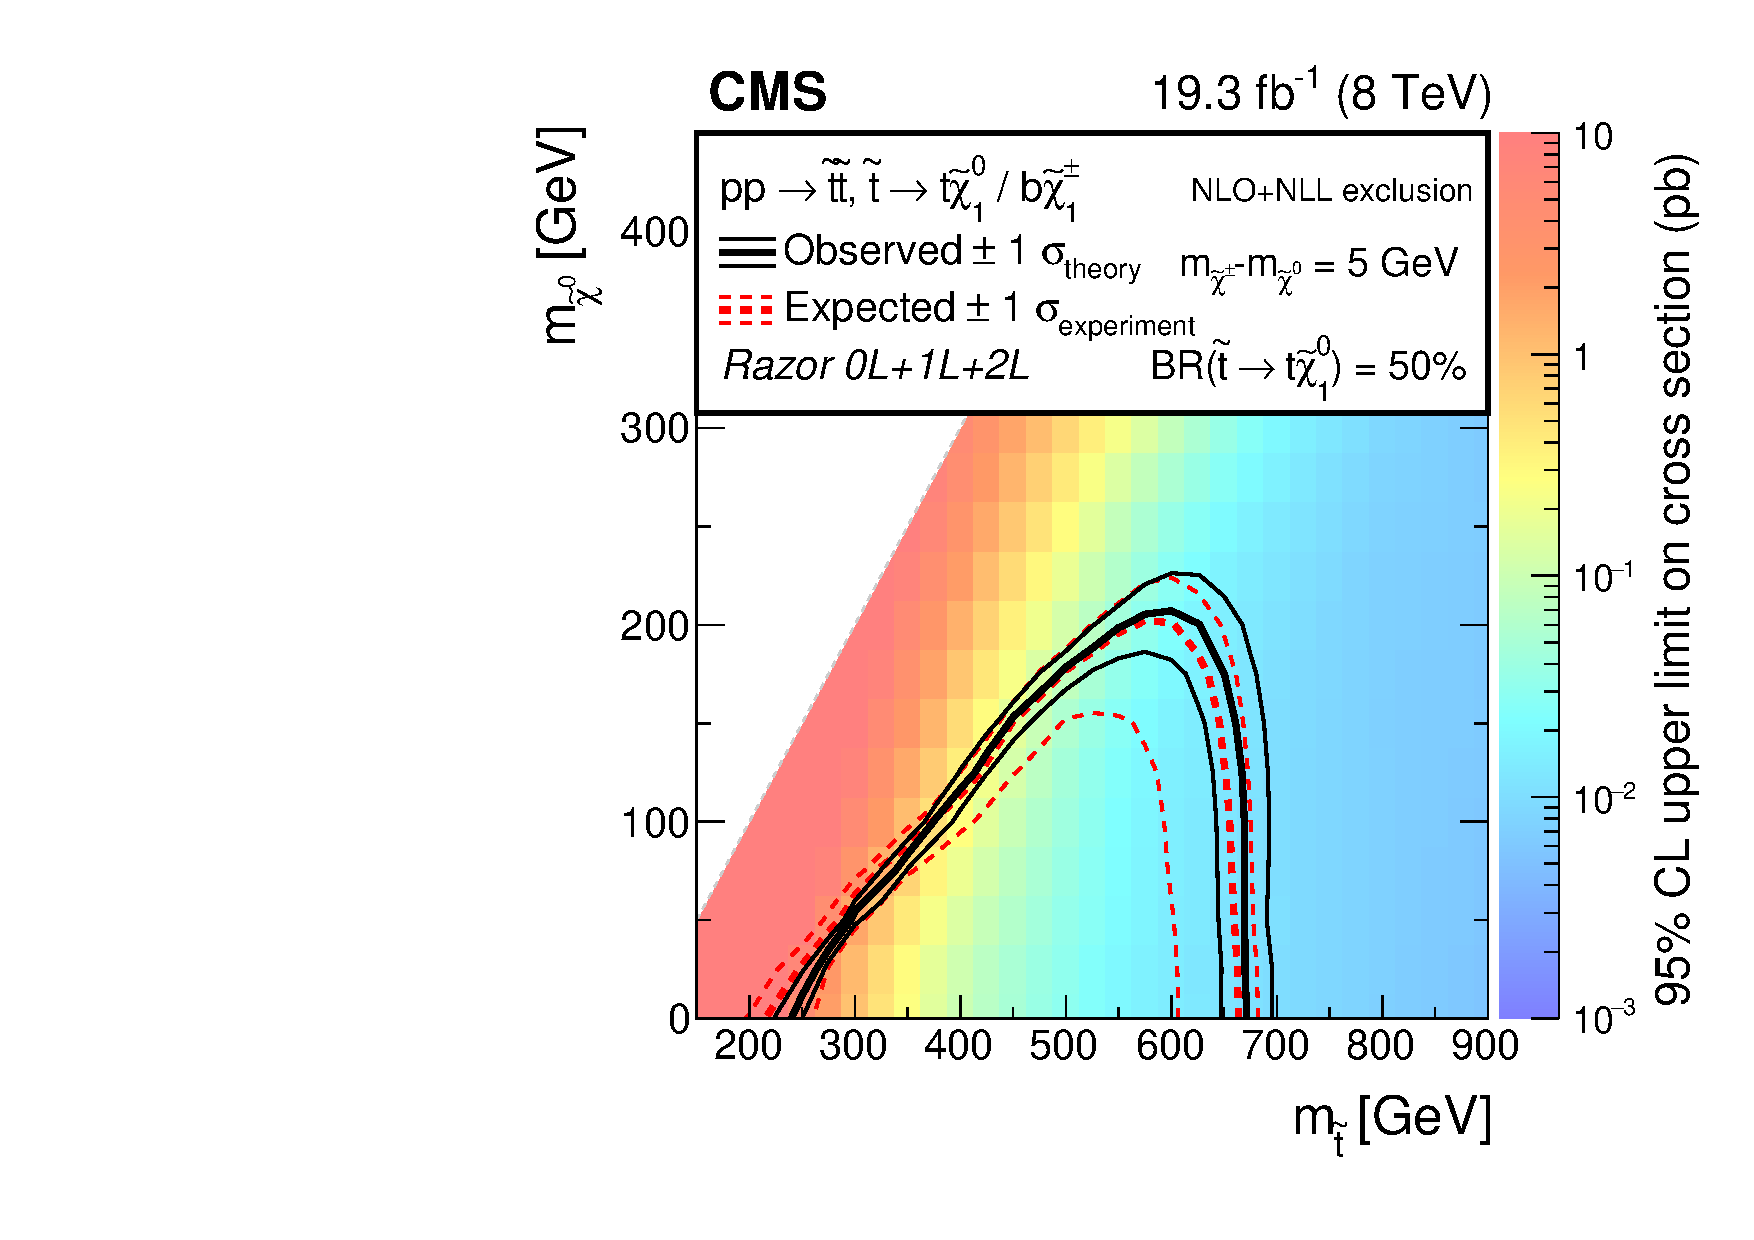
\includegraphics[width=0.49\textwidth]{figs/analysis8TeV/T2tbHybridNew0Lp1Lp2LXSEC.pdf}
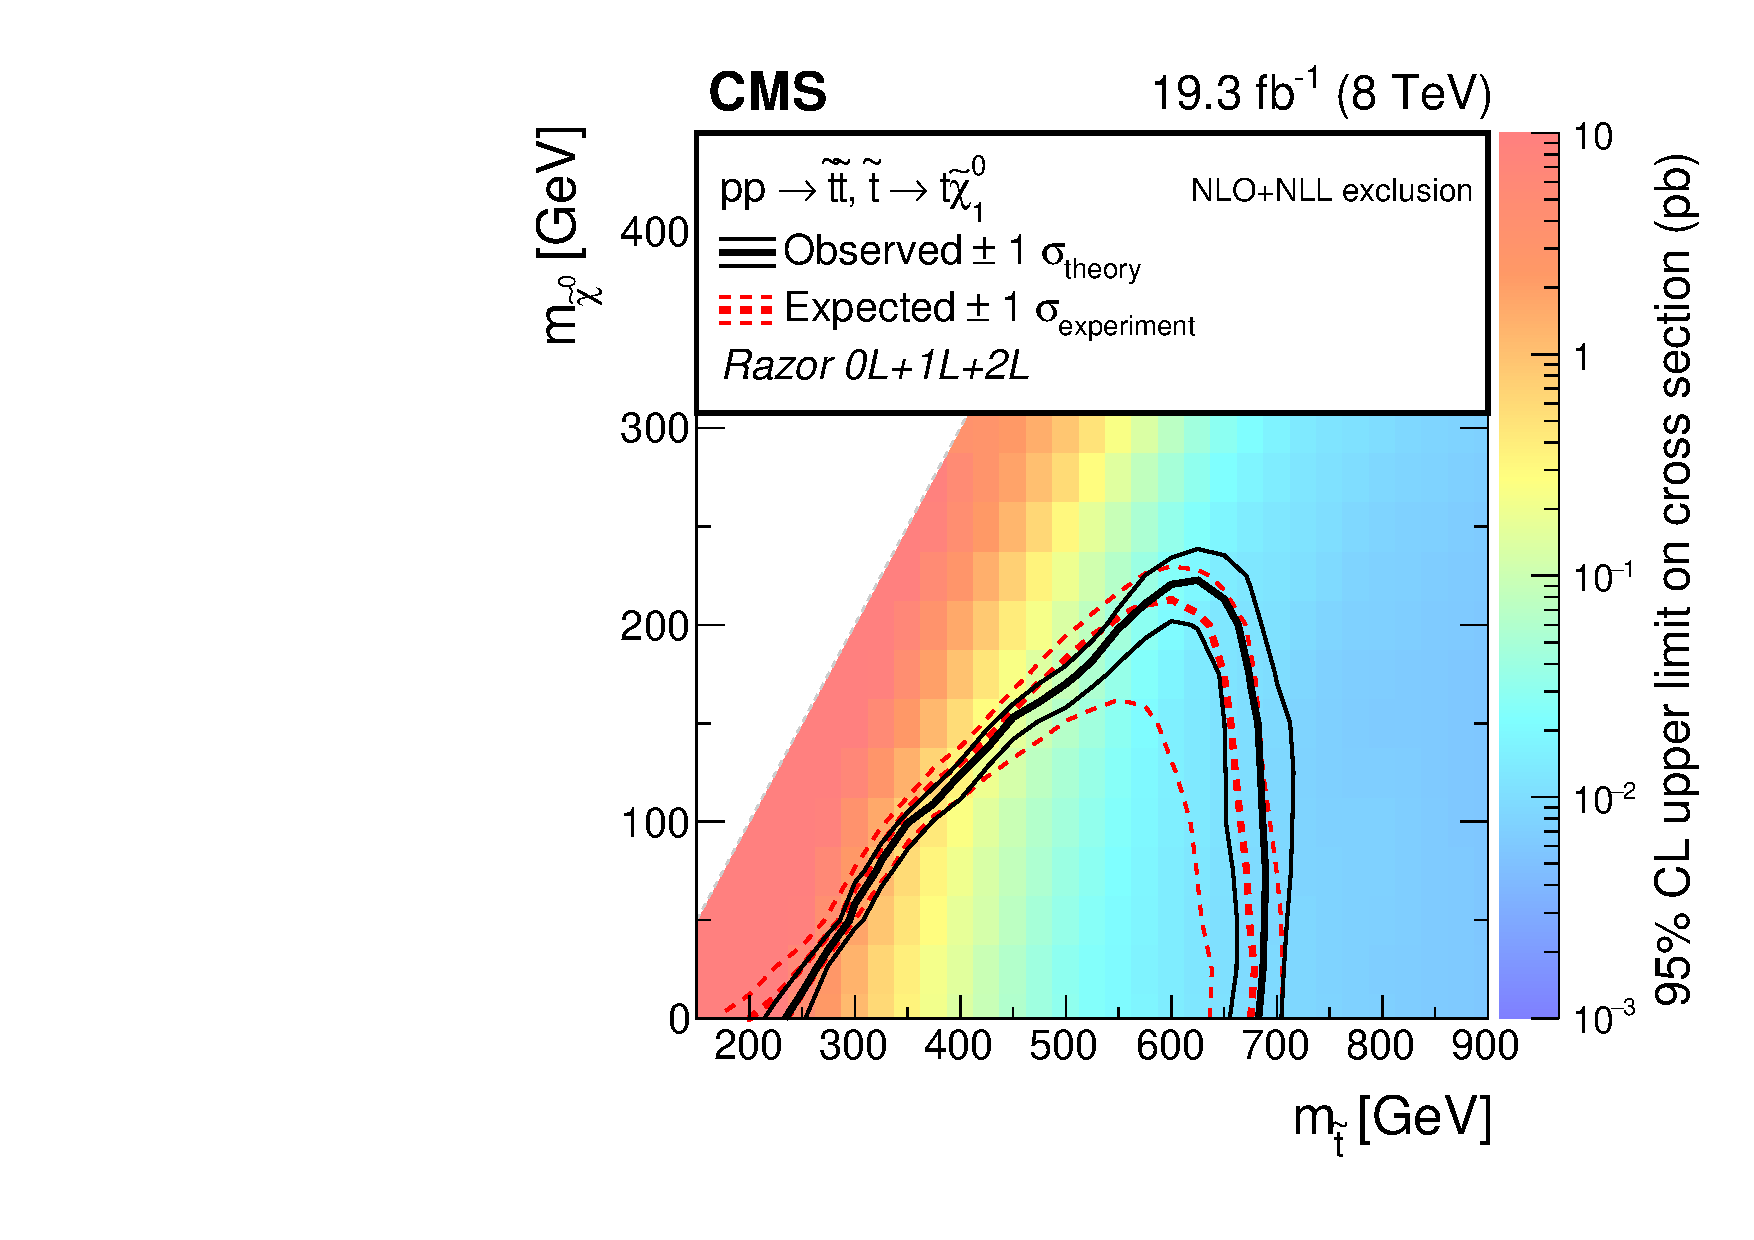
\includegraphics[width=0.49\textwidth]{figs/analysis8TeV/T2ttHybridNew0Lp1Lp2LXSEC.pdf}
\caption{Interpretation of the inclusive search with razor variables
  in the context of top-squark pair production models: (\cmsUpperLeft)
  T2bW$^{\ast}$, (\cmsUpperRight) T2tb, and (bottom) T2tt.  The limit for T2bW$^{\ast}$
  is derived using only the hadronic boxes, while the limits for the
  remaining models are derived using all nine boxes. The meaning of
  the color coding and the displayed contours is explained in the
  caption of Fig.~\ref{fig:gluino2D}.\label{fig:squark2D}}
\end{figure*}

\begin{figure}[tb!]
\centering
 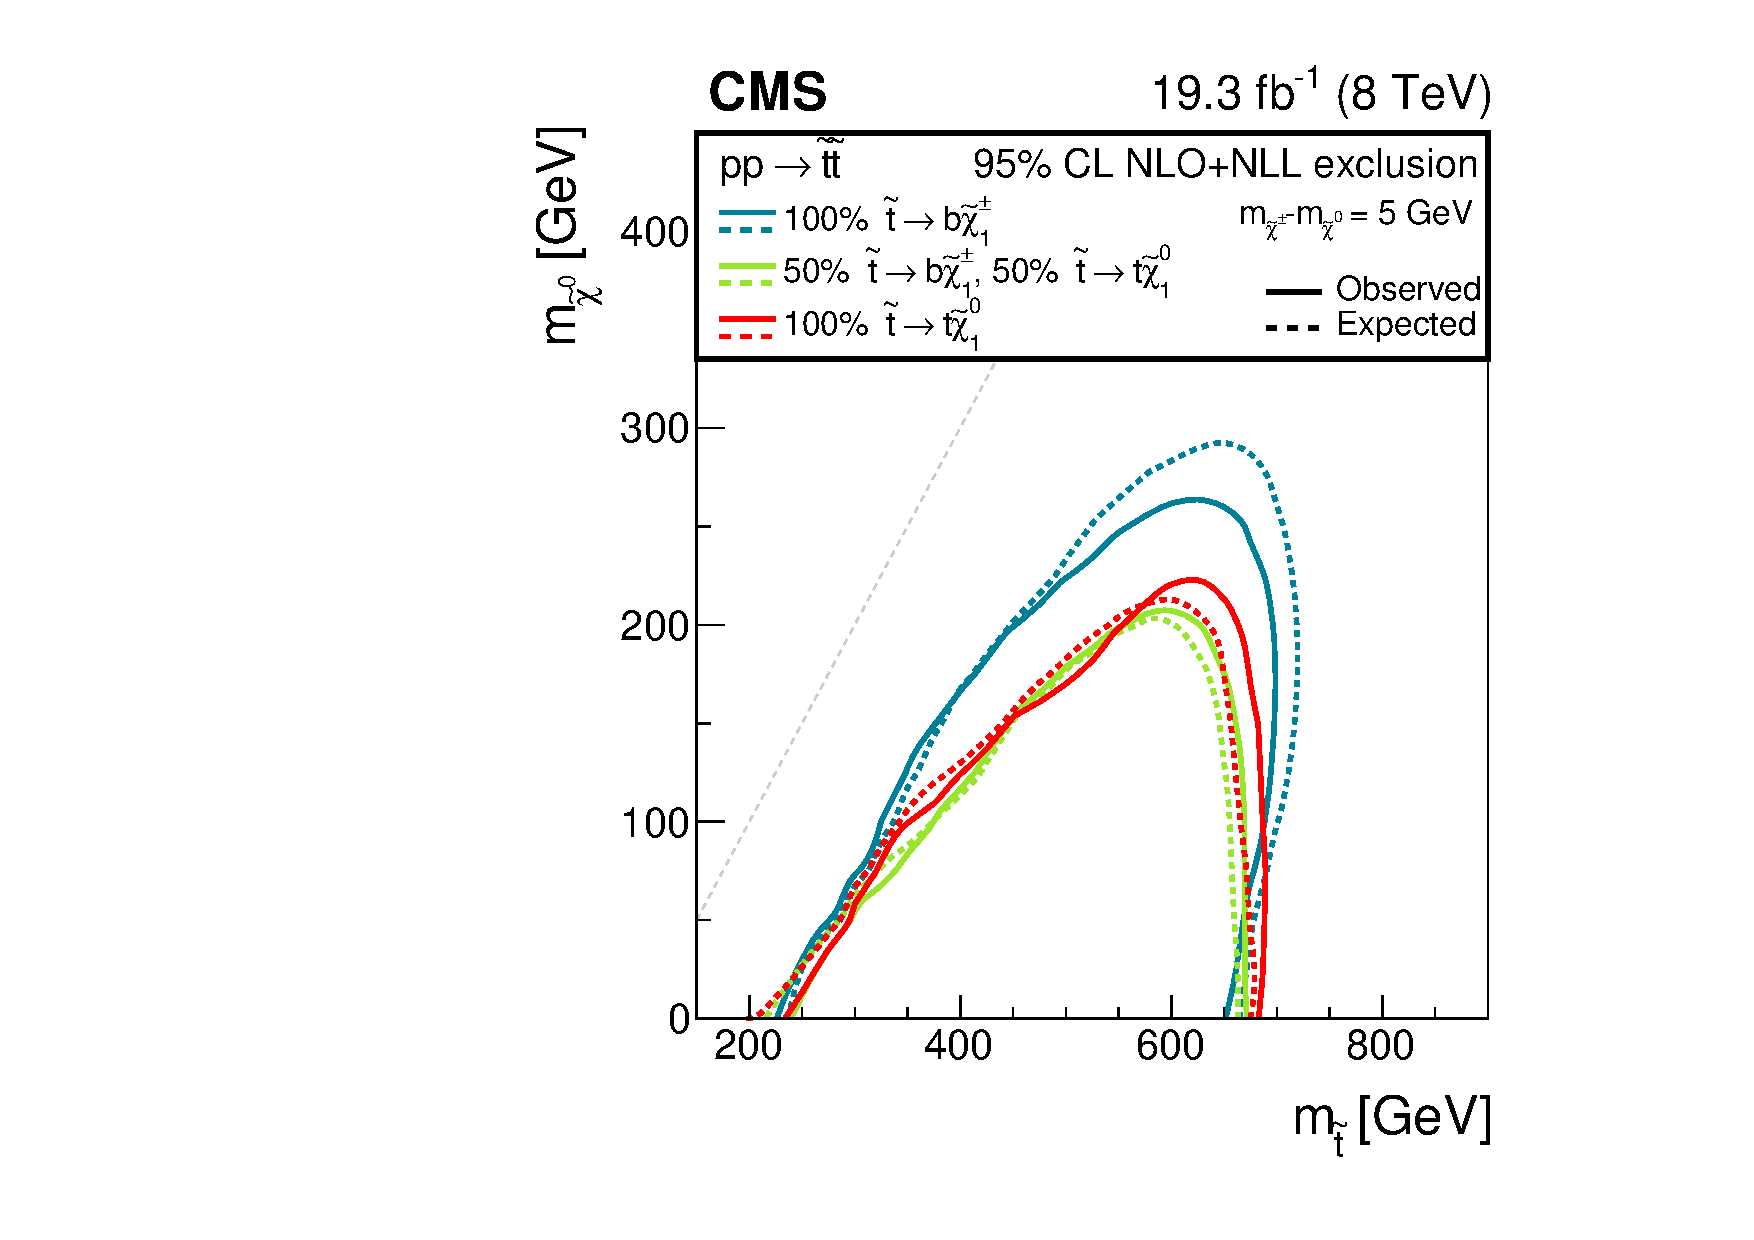
\includegraphics[width=\cmsFigWidth]{figs/analysis8TeV/T2HybridNew0Lp1Lp2LBARE.pdf}
 \caption{Top-squark mass limit at a 95\% \CL, obtained for different
   squark pair production models with the inclusive razor analysis in the
   context of the natural SUSY spectrum of
   Fig.~\ref{fig:spectrum}.\label{fig:stopSUMMARY}}

\end{figure}

A stronger limit on top-squark pair production is derived by combining
the hadronic boxes of the razor search with the results of the
exclusive single-lepton analysis~\cite{1LepMVA}. The exclusive
single-lepton search is conservatively assumed to only have
sensitivity when both top squarks decay to a top quark and a
neutralino. Figure~\ref{fig:combinedLimit} (\cmsLeft) presents the combined result obtained for the scenario where the top
squark only decays to a top quark and the lightest neutralino. For an
LSP mass of 100\GeV, the combination improves the constraint on the
top-squark mass from 660 to 730\GeV. This result provides the
most stringent limit on this specific simplified model.


Figure~\ref{fig:combinedLimit} (\cmsRight) presents a more generic limit on the
top-squark mass. We consider two decay modes for the top squark, as
indicated in Fig.~\ref{fig:spectrum}. We scan the relative branching
fractions, assuming that no other decay mode is allowed. The largest
excluded cross section (that is, the worst upper limit) is found for
each choice of the top-squark and neutralino mass. A
branching-fraction-independent limit is derived by comparing the
worst-case exclusion to the corresponding top-squark pair production
cross section. In this manner, top squarks decaying to the two
considered decay modes are excluded at a 95\% confidence level for
mass values $>$400\GeV and $<$645\GeV, assuming a neutralino mass of
100\GeV. Unlike other simplified model interpretations, this
interpretation is not based on a specific choice of branching
fractions. While a residual model dependence is present because only
two decay modes are considered, this result is more general than
previous constraints.

\begin{figure}[tb!]
\centering
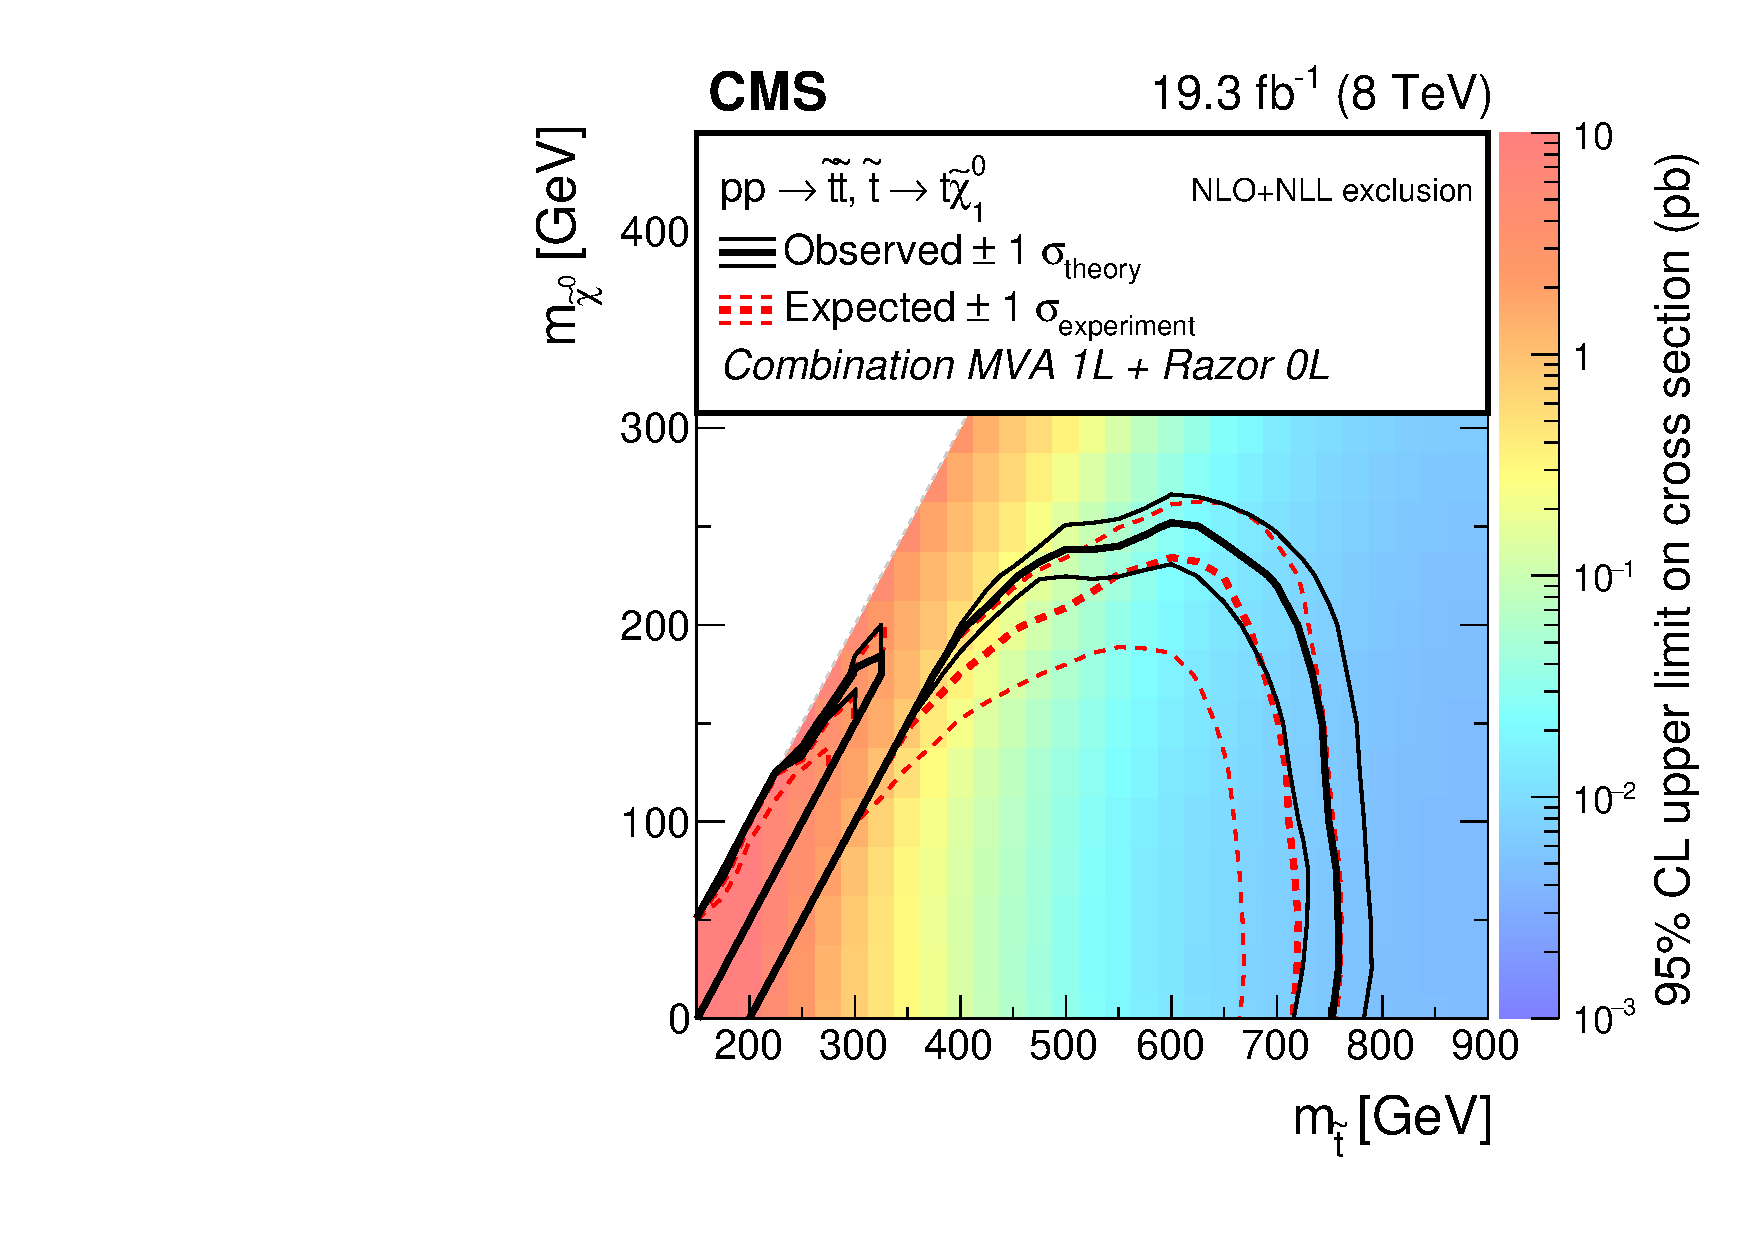
\includegraphics[width=0.49\textwidth]{figs/analysis8TeV/T2ttCOMBINED.pdf}
\includegraphics[width=0.49\textwidth]{figs/analysis8TeV/T2briCOMBINED.pdf}
\caption{Top-squark mass limit at a 95\% \CL, obtained combining the
  result of the hadronic razor boxes with the result of
  Ref.~\cite{1LepMVA} for (\cmsLeft) T2tt and (\cmsRight) independent of
  the branching fraction choice. The meaning of
  the color coding and the displayed contours is explained in the
  caption of Fig.~\ref{fig:gluino2D}.\label{fig:combinedLimit}}
\end{figure}

\section{Summary}
\label{sec:conclusion}
We present a search for supersymmetric particles using proton-proton
collision data collected by CMS in 2012 at $\sqrt{s} = 8\TeV$. The data set
size corresponds to an integrated luminosity of 19.3\fbinv. We
consider events with at least two jets, at least one of which is
identified as a \PQb-tagged jet, and study the event distribution in the
razor variables ($\MR$, $\Rtwo$). The data are
classified according to the muon, electron, jet, and \PQb-tagged jet
multiplicities.  No significant excess is observed with respect to the
standard model background expectations, derived from a fit to the data
distribution in low-$\MR$ and low-$\Rtwo$ sidebands.

The inclusive razor search is translated into 95\% confidence level
exclusion limits on the masses of the gluino and the top squark, in the
context of simplified ``natural'' SUSY models.  For a neutralino mass
of 100\GeV and depending on the branching fractions, the pair
production of gluinos and top squarks in multi-bottom, multi-top, and
mixed top-plus-bottom quark topologies is excluded for gluino masses
up to 1310\GeV and top-squark masses up to 660\GeV.  Using the
combined likelihood of the hadronic boxes of the razor search and the
single-lepton channels of the exclusive top-squark
search~\cite{1LepMVA}, the exclusion bound on the top-squark mass is
extended to 730\GeV for a top squark decaying to a top quark and to a
neutralino of mass 100\GeV.  Again assuming the neutralino mass to be 100\GeV, top
squarks decaying to the two considered decay modes are excluded at a
95\% confidence level for mass values between 400 and 645\GeV,
independent of the branching fractions.
